% ------------------------------------------------------------------------
% ------------------------------------------------------------------------
% ICMC: Modelo de Trabalho Acadêmico (tese de doutorado, dissertação de
% mestrado e trabalhos monográficos em geral) em conformidade com 
% ABNT NBR 14724:2011: Informação e documentação - Trabalhos acadêmicos -
% Apresentação
% ------------------------------------------------------------------------
% ------------------------------------------------------------------------

% Opções: 
%   Qualificação         = qualificacao 
%   Curso                = doutorado/mestrado
%   Situação do trabalho = pre-defesa/pos-defesa (exceto para qualificação)
% -- opções do pacote babel --
% Idioma padrão = brazil
	%french,	    	% idioma adicional para hifenização
	%spanish,			% idioma adicional para hifenização
	%english,			% idioma adicional para hifenização
	%brazil				% o último idioma é o principal do documento
	\documentclass[brazil]{packages/icmc}

% ---
% Pacotes Opcionais
% ---
\usepackage{minted}           % Usado para rotacionar o texto
\usepackage{rotating}           % Usado para rotacionar o texto
\usepackage[all,knot,arc,import,poly]{xy}   % Pacote para desenhos gráficos
% Este pacote pode conflitar com outros pacotes gráficos como o ``pictex''
% Então é necessário usar apenas um dos pacotes conflitantes


% ---
% Informações de dados para CAPA e FOLHA DE ROSTO
% ---
\titulo{\emph{Sharpener}: Ferramenta de correção automática de programas para o ensino de programação com workflow expandido.}
\autor[Abbud, P. M.]{Pedro Morello Abbud}
\orientador[Orientador:]{Prof.\ Dr.}{Dilvan de Abreu Moreira}
\coorientador{Prof.\ Dr.}{Orlando de A.\ Figueiredo}
\curso{Engenharia da Computação}
\area{Sistemas Computacionais} % Área de concentração do trabalho
\data{01}{10}{2019} % Data do depósito
% ---


% ---
% RESUMOS
% ---

% Resumo em português
% conter no máximo 500 palavras
\textoresumo{Propõe-se a construção de uma prova de conceito para uma ferramenta 
    de ensino a programação, que seja moderna e de código aberto.}{Ensino de programação, Sistemas \emph{Web}}


% ---
% resumo em inglês
% ---
\textoresumo[english]{
    Proposal for the creation of a proof of concept on a programming languages
    teaching tool, that is both modern and open source.
}{Programming language education, \emph{Web} systems}
% ---
% Configurações de aparência do PDF final
% ---
% alterando o aspecto da cor azul
\definecolor{blue}{RGB}{41,5,195}

% informações do PDF
\makeatletter
\hypersetup{
     	pagebackref=true,
		pdftitle={\@title}, 
		pdfauthor={\@author},
    	pdfsubject={\imprimirpreambulo},
	    pdfcreator={LaTeX with abnTeX2/ICMC-USP},
		pdfkeywords={\palavraschave}, 
		colorlinks=true,       		% false: boxed links; true: colored links
    	linkcolor=blue,          	% color of internal links
    	citecolor=blue,        		% color of links to bibliography
    	filecolor=magenta,      	% color of file links
		urlcolor=blue,
		bookmarksdepth=4
}
\makeatother
% --- 

% ----------------------------------------------------------
% ELEMENTOS PRÉ-TEXTUAIS
% ----------------------------------------------------------

% Inserir a ficha catalográfica
% \incluifichacatalografica[tex/fichaCatalografica.pdf]
\incluifichacatalografica


% Inserir folha de aprovação
% 
% Isto é um exemplo de Folha de aprovação, elemento obrigatório da NBR
% 14724/2011 (seção 4.2.1.3). Você pode utilizar este modelo até a aprovação
% do trabalho. Após isso, substitua todo o conteúdo deste arquivo por uma
% imagem da página assinada pela banca com o comando abaixo:
%
% \includepdf{folhadeaprovacao_final.pdf}
%
\begin{folhadeaprovacao}

  \begin{center}
    {\ABNTEXchapterfont\large\imprimirautor}

    \vspace*{\fill}\vspace*{\fill}
    {\ABNTEXchapterfont\bfseries\Large\imprimirtitulo}
    \vspace*{\fill}
    
    \hspace{.45\textwidth}
    \begin{minipage}{.5\textwidth}
        \imprimirpreambulo
    \end{minipage}%
    \vspace*{\fill}
   \end{center}
    
   Trabalho aprovado. \imprimirlocal, 24 de novembro de 2012:

   \assinatura{\textbf{\imprimirorientador} \\ Orientador} 
   \assinatura{\textbf{Professor} \\ Convidado 1}
   \assinatura{\textbf{Professor} \\ Convidado 2}
   %\assinatura{\textbf{Professor} \\ Convidado 3}
   %\assinatura{\textbf{Professor} \\ Convidado 4}
      
   \begin{center}
    \vspace*{0.5cm}
    {\large\imprimirlocal}
    \par
    {\large\imprimirdata}
    \vspace*{1cm}
  \end{center}
  
\end{folhadeaprovacao}
% ---

% DEDICATÓRIA / AGRADECIMENTO / EPÍGRAFE
% \textodedicatoria*{tex/pre-textual/dedicatoria}
\textoagradecimentos*{tex/pre-textual/agradecimentos}
% \textoepigrafe*{tex/pre-textual/epigrafe}

% Inclui a lista de figuras
\incluilistadefiguras

% Inclui a lista de tabelas
% \incluilistadetabelas

% Inclui a lista de quadros
% \incluilistadequadros

% Inclui a lista de algoritmos
% \incluilistadealgoritmos

% Inclui a lista de códigos
% \incluilistadecodigos

% Inclui a lista de siglas e abreviaturas
% \incluilistadesiglas

% Inclui a lista de símbolos
% \incluilistadesimbolos

% ----
% Início do documento
% ----
\begin{document}

% ----------------------------------------------------------
% ELEMENTOS TEXTUAIS
% ----------------------------------------------------------
% \textual

\chapter{Introdução}
\label{chapter:introducao}
\section{Motivação e Contextualização}
Nas últimas décadas, o interesse por programação cresceu de forma extraordinária 
e cursos introdutórios mostram-se cada vez mais populares. No entanto, 
cursos de programação ainda são considerados difíceis e, com frequência,
possuem taxas de desistência elevada. Iniciantes sofrem de uma 
vasta gama de défices e dificuldades, desde a compreensão de constructos 
básicos de uma linguagem de programação à elaboração de planos
para resolver um dado problema \ \cite{robins2003learning}.

Estudos concluem, de forma semelhante, que alunos, 
mesmo tendo aprendido a sintaxe e semântica de uma linguagem 
de programação, tendem a falhar em compor os blocos fundamentais 
estudados em programas válidos. Parte deste problema é abordada por 
\citeonline{davies1993models}, que faz uma distinção de duas partes 
essenciais no aprendizado em programação: 
conhecimento e estratégia. Denota-se conhecimento em programação como a parte declarativa 
do conhecimento, por exemplo, saber que existe um constructo chamado \emph{for} na linguagem 
e seu propósito. Já estratégia em programação seria empregar de forma adequada o conhecimento 
em face de um problema, como o uso pertinente de um \emph{for} em um programa.
\citeonline{davies1993models} defende que grande parte das abordagens em ensino 
tendem a investir excessivamente na parcela de conhecimento em programação, muitas 
vezes deixando de lado o aspecto de estratégia.

Em vista do imenso desafio que é o ensino de programação a iniciantes, diversas ferramentas 
foram desenvolvidas para dar apoio pedagógico ao professor nesta tarefa.  
Estas ferramentas, em grande parte, são sistemas de juízes \emph{online}, 
que consistem em sistemas capazes 
de receber códigos desenvolvidos pelos usuários como resposta a um determinado problema, mas 
com a capacidade de dar \emph{feedback} imediato ao usuário, informando 
se o código está correto ou não, através de análise sintática e testes automatizados.

Já existe uma grande variedade em juízes \emph{online} disponíveis na literatura científica,
tais como: 
\hyperref[link:the_huxley]{\emph{The Huxley}} [\citeonline{de2013ferramenta}], 
	\hyperref[link:code_bench]{\emph{CodeBench}} [\citeonline{galvao2016juiz}],  
	\hyperref[link:uva_judge]{\emph{UVa Online Judge}} [\citeonline{revilla2008competitive}], 
	\hyperref[link:feeper]{\emph{feeper}} [\citeonline{alves2014ambiente}], 
	\hyperref[link:uri_judge]{\emph{URI Online Judge}} [\citeonline{bez2014uri}], 
	\hyperref[link:boca]{\emph{BOCA}} [\citeonline{de2004boca}],
	\hyperref[link:we_run_codes]{\emph{RunCodes}},
	\hyperref[link:sphere_judge]{\emph{Sphere Online Judge}},
	\hyperref[link:hacker_rank]{\emph{HackerRank}}, 
	\hyperref[link:code_chef]{\emph{CodeChef}}, 
	\hyperref[link:interview_bit]{\emph{InterviewBit}}, 
	\hyperref[link:kattis]{\emph{Kattis}}, 
	\hyperref[link:leet_code]{\emph{LeetCode}}, 
	\hyperref[link:codin_game]{\emph{CodinGame}}, 
	\hyperref[link:code_signal]{\emph{CodeSignal}}, 
	\hyperref[link:code_wars]{\emph{CodeWars}}, 
	\hyperref[link:exercism]{\emph{Exercism}}, 
	entre tantos outros.

Boa parte dessas ferramentas consiste em serviço gratuito oferecido ao aprendiz,
e com poucos recursos de acompanhamento por parte dos professores.
Outra parte, sim, é direcionada para situações acadêmicas, mas com 
\emph{workflows} de submissão e correção de programas rígidos;
qualquer intenção de personalizar uma típica ferramenta desse gênero
implica alterar o código-fonte.

O sistema que é tema do presente trabalho, o \emph{Sharpener}, surgiu do
anseio de se fazer pequenas adaptações a ferramentas de apoio a disciplinas
de programação.
Um problema observado é que alguns alunos não sabem como dar um próximo passo
na resolução de um exercício;
muitas vezes, eles precisam de um empurrão (como uma dica) para prosseguir.
Em aulas com muitos alunos, o professor nem sempre é capaz de proporcionar
esse tipo de acompanhamento e atenção, devido às limitações evidentes.
A questão passa a ser, então, se uma ferramenta poderia prover ao aluno
algum tipo de apoio, de forma que ele, seguindo a ferramenta, pudesse
explorar possibilidades e alternativas que o impulsionassem na continuação
do exercício; o aluno teria, com isso, uma relativa autonomia no aprendizado.

A solução mais imediata é capacitar a ferramenta a entregar dicas conforme
o aluno as solicita. Para isso, o professor precisaria ter alimentado o sistema
com dicas no mesmo momento em que teria carregado o enunciado do exercício.
Uma ideia similar é entregar ao aluno, de uma vez, a resposta completa do problema.
Muitos alunos têm uma ansiedade por ver respostas. 
A experiência de ver a resposta de um problema não resolvido pode ser um momento
de intensa aprendizagem.
Em vez de coibir isso, a ferramenta pode estimular, compensando com a 
apresentação, em seguida, de um exercício equivalente e alternativo.
Uma terceira proposta, ainda no espírito de fornecer algum tipo de dica,
é conduzir o aluno numa solução incremental do problemas, propondo pequenos
passos (incrementos) rumo à solução.
Com \emph{workflows} como esses, além do efeito pretendido de dar alguma 
autonomia ao aluno, há um efeito colateral que é a possibilidade de o professor
ter acesso ao histórico de consultas do aluno, podendo fazer uma avaliação
mais rica do seu percurso de aprendizagem.

Em vez de adaptar ferramentas existentes cujo código fosse aberto,
optou-se por criar um protótipo de uma ferramenta nova como prova de conceito.
O foco desse desenvolvimento passou a ser as componentes arquiteturais 
principais do sistema, como o servidor e sua API de acesso, e
uma ferramenta cliente de linha de comando.
Embora a contribuição pretendida aqui resida no domínio do
ensino de programação e suas ferramentas de apoio,
levando em conta que se trata de um Trabalho de Conclusão de Curso,
é inevitável tentar apresentar neste documento
alguns aspectos predominantes no desenvolvimento do protótipo, 
tais como: \emph{design} de APIs Web, estilo arquitetural \emph{REST}, computação em nuvem, autenticação federada,
e as principais decisões de projeto.
O escopo proposto inicialmente revelou-se excessivo, considerando-se o prazo de
um semestre letivo, e este trabalho passou a ser apenas a etapa inicial do
desenvolvimento do \emph{Sharpener}.

\section{Objetivos}
Pretende-se neste trabalho desenvolver um protótipo, como prova de conceito, de um sistema para apoio 
ao ensino de programação em salas de aula, que forneça apoio a estudantes estagnados no
desenvolvimento de exercícios, apoio esse que se manifesta
na forma de dicas, respostas, exercícios alternativos e
passos incrementais.

Em termos de software, pretende-se desenvolver minimamente uma arquitetura baseada em Web,
com um servidor acessível por \emph{API REST}, com suporte a autenticação federada, 
compatível com computação em nuvem, um cliente de linha de comando para funcionalidades
diretamente ligadas aos exercícios, e um cliente web para
funcionalidades administrativas básicas.

\section{Organização}
O cerne do trabalho é apresentado no \Cref{chapter:desenvolvimento}. Ali se encontram: a descrição
dos \emph{workflows} do principais atores (Aluno e Professor), seja na interface de linha de comando ou
na interface Web; e a descrição da API Web.

Dado o caráter de desenvolvimento de software do presente trabalho, diversos tópicos
foram mobilizados para a sua execução, entre metodologias, técnicas e ferramentas.
No \Aref{chapter:implementacao}, traça-se um panorama de todo o processo.
O \Cref{chapter:metodos} contém uma apresentação de alguns tópicos selecionados,
assim como o \Aref{chapter:cicd}.

Por fim, no \Cref{chapter:conclusao} estão as conclusões e contribuições do projeto, 
seguidas dos trabalhos futuros.


\chapter{Métodos, Técnicas e Tecnologias Utilizadas}
\label{chapter:metodos}
\section{Considerações Iniciais}
Este capítulo tem como propósito fornecer o embasamento teórico necessário 
para o entendimento da construção do sistema proposto. Aqui é contido uma
descrição detalhada das técnicas, métodos e tecnologias utilizadas, assim  
preparando o leitor para o conteúdo dos próximos capítulos.


\section{Design de \emph{API}s}
Separação de conceitos, traduzido do termo \emph{Separation of Concerns}, é uma temática 
chave na arquitetura cliente-servidor da internet. Parte do porquê a internet funciona tão bem
foi a preocupação, desde sua concepção, de uma interface uniforme que, desde que respeitada, 
 daria liberdade aos desenvolvedores de implementar, em qualquer linguagem ou tecnologia,
 um de seus componentes. 

Apesar do sucesso na separação de conceitos entre as responsabilidades que o navegador 
e o servidor empregam, a mesma preocupação não foi replicada entre interfaces e 
funcionalidades que o servidor expõe. 
Com frequência existe um alto acoplamento entre a interface, \emph{Frontend},
e o servidor, \emph{Backend}, o que resulta em uma interface não uniforme para interação 
dos recursos que deveriam estar expostos. Define-se aqui um recurso como qualquer conceito 
na internet que pode ser referenciado por um identificador único e manipulado por uma interface uniforme 
\ \cite{masse2011rest}.

A solução, que leva ao desacoplamento, é a interação com estas
funcionalidades través de uma \emph{API}, \emph{Application Programming Interface},
exposta pelo \emph{backend}, que provê formas padronizadas 
de acesso. Aqui não somente ganhamos portabilidade, já que possibilitamos que não só 
um tipo de cliente, navegadores, saibam como acessar nossos recursos, mas ganhamos espaço 
para criar uma camada de abstração do serviço \emph{Web}, modelando-o em recursos.
Estes recursos não serão projetados como uma cópia da organização de dados ou funcionalidades 
presentes no \emph{backend} mas em representações que sejam de fácil consumo e de entendimento 
ubíquo pelo lado do cliente.

O desafio de criar bons serviços na internet pode ser facilitado se empregarmos estilos 
arquiteturais já existentes. Aqui definimos estilos arquiteturais como 
um conjunto coordenado de restrições arquiteturais. \\
Um destes estilos arquiteturas que tem ganhado cada vez 
mais tração se chama \emph{REST}, \emph{Representational State Transfer}, ou em português,
\emph{Transferência Representacional de Estado}. Cunhado por \citeonline{fielding2000architectural}, 
o termo evoca como um sistema na \emph{Web} deveria se comportar, uma máquina de estados 
virtuais em que o usuário progride através da seleção de identificadores únicos, que identificam 
recursos, e verbos \emph{HTTP}
que operam sobre estes recursos.

As restrições na arquitetura impostas pelo estilo \emph{REST} são agrupadas em seis categorias:
\begin{description}
\item[Cliente-servidor:] A separação dos papéis do cliente e servidor deve ser clara para 
  que estes possam ser projetados e implementados de forma independente. A interação 
  entre eles só acontece na forma de requisições, que são iniciadas pelo cliente. 
  Servidores devem mandar respostas apenas como reações de requisições dos clientes.
\item[Interface uniforme:] interfaces \emph{REST} possuem quatro  restrições:
identificação de recursos, manipulação de recursos através de representações, 
mensagens auto-descritivas e hipermídia como motor de estado da aplicação, \emph{HATEOAS}.\\
A primeira dita que cada recurso precisa ser endereçável 
por um identificador único, \emph{URI}, \emph{Unique Resource Identifier}.\\
Este 
recurso pode ser representado de diversas formas, seja em formato \emph{HTML}, que é mais adequado para 
um navegador,
ou formato \emph{JSON}, que é mais apropriado para consumo de outro programa. Percebe-se aqui 
que a representação é apenas uma forma de interagir com o 
recurso,  não o próprio recurso. Isto é o que dita a segunda regra. \\
No consumo de uma \emph{API}, o cliente especifica um recurso e seu estado 
desejado, enquanto o servidor deve responder com o recurso e seu estado real. 
Esta troca de mensagens  deve ser feita utilizando \emph{headers} e 
códigos de estado \emph{HTTP} que descrevam o estado 
do recurso e metadados correspondentes, de forma que as mensagens sejam auto-descritivas.\\
A última restrição, \emph{HATEOAS}, ajuda a aumentar a visibilidade e descoberta de recursos 
relacionados na \emph{API}, que ajudam o cliente a navegar dinamicamente nos recursos expostos.
Assim, quando referenciam-se outros recursos, também são fornecidos seus identificadores únicos 
e verbos aceitos para aquela rota.
\item[Sistema em camadas:] Restringe-se o comportamento dos componentes em camadas, em que 
  cada camada só pode interagir com subjacentes. 
  Entre as chamadas do cliente que requisita uma representação de um estado de um recurso, e 
  o servidor que processa a requisição, pode haver vários servidores entre eles. Estes 
  servidores podem prover um camada de segurança, \emph{cache}, balanceamento de carga ou 
  outras funcionalidades. Estas camadas não devem afetar a requisição ou resposta e nem o cliente 
  nem servidor precisam estar cientes se elas existem ou não.
\item[Protocolo sem estado:] O servidor não deve lembrar absolutamente nada do usuário que 
  utiliza sua \emph{API}. Isto implica que toda requisição individual precisa conter toda 
  informação necessária para que o servidor processe e retorne uma resposta. Esta restrição 
  visa aumentar a escalablidade, visibilidade e confiabilidade do sistema. Escalabilidade pois 
  permite que haja \emph{caching} de respostas e que o servidor possa desalocar recursos 
  físicos entre requisições, visibilidade pois sistemas que monitoram requisições não 
  precisam olhar além de uma requisição, pois elas contêm todo o dado necessário 
  para entender a natureza desta, e a confibilidade pois a recuperação de falhas 
  parciais se torna mais simples \ \cite{kendall1994note}.
\item[Cache:] O servidor deve declarar quais dados podem ser guardados em \emph{caches}. 
  \emph{Caches} ajudam a reduzir a latência percebida pelo cliente, aumentam a disponibilidade 
  e confiabilidade de serviços e mitigam a carga de trabalho do servidor. Em resumo, 
  \emph{caches} reduzem todos os custos associados a um serviço na \emph{internet}.
\item[Código sob demanda:] A internet faz bastante uso de código sob demanda, que possibilita 
  que o servidor transfira executáveis, tais como \emph{scripts} e \emph{plugins}, para a 
  execução do lado do cliente. Apesar de proposto por \citeonline{fielding2000architectural}, 
  esta restrição tende a estabelecer um acoplamento de tecnologias entre servidor e cliente. 
  Por este motivo ``código sob demanda'' é a única restrição imposta pelo estilo arquitetural 
  \emph{REST} que é considerada opcional.
\end{description}

O maior desafio no projeto de uma \emph{API} é abstrair componentes do sistema
em recursos. O modelamento destes recursos estabelece os aspectos chaves da sua \emph{API}
e é semelhante ao processo de modelar um banco de dados relacional ou mesmo o modelamento 
clássico de um sistema orientado a objetos.

No processo de modelagem de recursos, rotineiramente começa-se pensando em arquétipos de 
recursos. Estes arquétipos nos ajudam a comunicar de forma consistente 
as estruturas que são frequentemente encontradas em \emph{Designs} de \emph{REST APIs}.
Idealmente, cada recurso pertence a apenas um dos seguintes arquétipos: \emph{document}, 
\emph{collection}, \emph{controller} e \emph{store}.

\emph{Document} é o arquétipo base de todos os outros, todos os outros arquétipos são especializações 
deste. Sua representação tipicamente inclui campos com dados ou \emph{hiperlinks} para outros 
recursos. \emph{Collection} é um diretório de outros recursos em que clientes podem recuperar 
ou, possivelmente, adicionar novos itens à coleção. Já \emph{Stores} são recursos que permitem 
que usuários guardem novos recursos, de forma que o próprio cliente escolha o 
identificador daquele recurso. Para recursos que se parecem mais como procedimentos que 
não se encaixam nos métodos padrões \emph{CRUD} (\emph{create, retrieve, update, delete}),
  o arquétipo \emph{Controller} é adequado. Todos estes arquétipos 
  contêm recomendações de como o identificador único deve ser escolhido, para que seja 
  claro a quem consome a \emph{API} de qual arquétipo se trata aquele recurso.

  \section{\emph{Python} e \emph{Flask}}
  Python é uma linguagem com sintaxe clara e concisa, favorecendo a legibilidade do 
  código-fonte, o que a torna uma linguagem extremamente produtiva. A linguagem incluí 
  diversas estruturas e módulos de alto nível e, por ser,
  segundo \hyperref[link:exercism]{\emph{a pesquisa anual de desenvolvedores 
      do site \emph{StackOverflow}}},
  uma das linguagens mais populares e amadas do mundo, possuí uma infinidade 
  de excelentes \emph{Frameworks} e bibliotecas de terceiros, que podem ser instalados 
  de forma simples e gratuita. 

  A linguagem incluí vários recursos de outras linguagens 
  modernas, tais como geradores, instropecção, persistência, metaclasses e unidades de 
  teste. Multiparadigma,
  a linguagem é feita para suportar programação modular e funcional, 
  tal como orientação a objetos.
  A linguagem é interpretada através de 
  \emph{bytecode}s pela máquina virtual do \emph{Python}, tornando seu código 
  excepcionalmente portável, e, como conta com tipagem dinâmica, é muito adequada 
  para prototipação \ \cite{borges2014python}. 

  Sua sintaxe clara torna fácil seu aprendizado, mesmo por iniciantes. 
  Além de ser largamente utilizada no desenvolvimento de sistemas, a linguagem é muito utilizada 
  para automatização de tarefas, por meio de \emph{scripts}. Também se integra 
  muito bem com outras linguagens, como \emph{C} ou \emph{Fortran}, fazendo-se 
  uma ótima linguagem para a escrita de \emph{wrappers}. \emph{Python} é um 
  \emph{software} de código aberto e é largamente utilizado na indústria, 
  por grandes empresas como: \emph{Microsoft}, \emph{Yahoo}, \emph{Google}, \emph{Disney}, 
  entre tantas outras.

  \emph{Python} é largamente utilizado para a construção de aplicações \emph{Web}, normalmente 
  desenvolvidos em algum tipo de \emph{framework}, sendo \emph{Django} a escolha mais comum.
  \emph{Django} conta com todas as ferramentas necessárias para o desenvolvimento 
  embutidas em seu \emph{framework}, como \emph{ORM}, \emph{Object Relation Mapper}, 
  soluções para autenticação e autorização, e um sistema de administração. Ao oferecer
  uma solução completa, perde-se em desempenho na aplicação e inflexibiliza-se seu 
  desenvolvimento. Para aqueles 
  que querem construir uma aplicação enxuta e de forma menos opinada, sugere-se um
  \emph{microframework Web}. 

  O mais popular \emph{microframework web} escrito em Python se chama \emph{Flask}.
  Denomina-se ``\emph{micro}'' devido as poucas escolhas que foram feitas 
  em sua implementação,
  deixando a cargo do desenvolvedor a implementação dos módulos que se mostrem 
  necessários. A abordagem minimalista possibilita o surgimento de um ecossitema de 
  pacotes diverso, em que o desenvolvedor opta por pacotes que são mais adequados a 
  necessidade do projeto, ao invés de seguir decisões tomadas pelo \emph{framework}.

  \section{O padrão \emph{OAuth}}
  Apesar de vivermos em um mundo que depende, cada vez mais, de serviços digitais,
  a maior parcela dos usuários ainda não se educaram ou 
  não seguem boas práticas de segurança na \emph{internet}. Não é infrequente que se 
  usem as mesmas credenciais em múltiplos serviços, mesmo que o usuário 
  não tenha meios de averiguar que suas informações são manuseadas e armazenadas de forma 
  adequada.

  Uma das possíveis soluções para uma melhor gestão de identidade na \emph{internet} 
  é o uso de identidades federadas \cite{208723}. Uma identidade federada é um meio 
  de uma pessoa vincular sua identidade eletrônica e atributos pessoais 
  a múltiplas partes distintas. Esta solução traz benefícios como mais garantias
  de segurança no armazenamento de credencias, menos sobrecarga de responsabilidade 
  para desenvolvedores de aplicações e uma melhor experiência para o usuário, já que se 
  diminui o atrito na criação e gerenciamento de múltiplas contas.

  O modelo de serviço federado pode ser dividido em duas componentes necessárias: 
  o provedor de identidade e o provedor de serviço. Ambas as partes cumprem papéis 
  distintos e sem qualquer uma delas não temos uma solução de identidade federada. 
  Para que a solução funcione, deve haver um relacionamento de confiança entre 
  o provedor de identidade e o provedor de serviço. Caso o provedor de identidade 
  não confie no provedor de serviço, este não o confiará os dados de usuários.
  Caso o provedor de serviço não confie no provedor de identidade, 
  também não confiará nas informações advindas dele.

  O provedor de identidade é quem mantém as informações de identidade. Usuários 
  se autenticam diante ao banco de credenciais do provedor, que então libera as
  informações relativas àquele usuário ao provedor de serviço que iniciou o processo 
  de autenticação. O provedor de serviço é aquele que provê serviços a usuários, 
  estes sendo aplicações, serviços de infraestrutura ou serviços de dados. Com a popularização 
  do modelo de computação em nuvem, cada vez mais usuários entram em contato com algum dos três 
  principais modelos de serviço em nuvem,  \emph{Infrastructure as a Service} (\emph{IaaS}), 
  \emph{Platform as a Service} \emph{PaaS} e \emph{SaaS}, \emph{Software as a Service}, 
  todas as quais dependem de um modelo de serviço federado \cite{rountree2012federated}.

  Existem vários padrões que implementam o modelo de serviço federado, as mais famosas sendo:
  \emph{SAML} (Security Assertion Markup Language), \emph{OAuth}, \emph{OpenID} 
  e \emph{Windows Identity Foundation}. O 
  padrão que tem ganhado mais adeptos, pela sua abordagem simples porém robusta,
  é o padrão \emph{OAuth}, que já conta com quatro revisões, sendo a última
  \emph{OAuth 2.0}. 

  \emph{OAuth 2.0} é um padrão aberto criado para suportar autorização de forma segura. 
    Existem quatro papéis definidos pelo padrão: servidor de autorização, 
  servidor de recurso, dono do recurso, comumente chamado de usuário, e o cliente, 
  que no contexto do \emph{OAuth 2.0} é uma aplicação que quer ser autorizada a 
  acessar um recurso do usuário. 

  O padrão suporta vários fluxos de autorização dependendo das capacidades 
  e grau de confiança que o servidor de autorização possui em um cliente.
  Caso o cliente tenha a capacidade de armazenar um segredo em comum com o 
  servidor de autorização, o fluxo de concessão do código de autorização \emph{(Authorization Code Grant)} 
  pode ser utilizado. Se ele não possui essa capacidade, como no caso de aplicações 
  que são executadas no computador do usuário, o fluxo implicito \emph{(Implicit Grant)} 
  pode ser utilizado. Se o cliente pode ser confiado com as credenciais do usuário, 
  comum em aplicações da mesma empresa, 
  ele pode utilizar o fluxo de senha do dono do recurso \emph{(Resource Owner Password Grant)}.

  Alem disso, o \emph{OAuth 2.0} permite que clientes obtenham permissão para acessar 
  recursos que não são relacionados a nenhum usuário utilizando o fluxo de credenciais 
  de cliente \emph{(Client Credentials Grant)}. 
  A maioria das aplicações Web, por possuirem servidores capazes de manter 
  um segredo em comum com o servidor de autorização, fazem o uso do fluxo de código de acesso,
  que é ilustrado pela \fref{fig:web_flow} e definido por \citeonline{hardt2012rfc}. 

  O fluxo de concessão de código de acesso começa quando um usuário, dono de um recurso, escolhe 
  fazer \emph{login} ou atrelar sua conta do servidor de autorização em uma aplicação. A aplicação 
  encaminha o usuário ao servidor de autorização e o usuário preenche suas credencias  
  e autoriza a aplicação a acessar um determinado 
  escopo de recursos. Em seguida, o servidor de autorização emite um código de autorização, 
  que geralmente expira em minutos. A aplicação, em posse do código de autorização, requisita 
  diretamente ao servidor de autorização um código de acesso. Com o código de acesso, a aplicação agora 
  pode acessar recursos protegidos do servidor de recursos, até que este código expire.

  Existem alguns detalhes que garantem a segurança do fluxo anterior. Quando a aplicação requisita 
  o servidor de autorização por um código de autorização, ela informa um identificador de cliente, que 
  indica sua identididade, uma \emph{url} de retorno, que é para onde o servidor de autorização mandará 
  o código de acesso e uma cadeia de caracteres aleatórios que será usado para validar se a requisição 
  veio do servidor de autorização. Caso na requisição a \emph{url} de retorno informada seja diferente 
  da cadastrada pela aplicação no servidor de autorização previamente, a requisição é abortada. No 
  recebimento da resposta do servidor de autenticação, caso a cadeia de caracteres aleátorios não seja a mesma 
  da enviada, aborta-se o processo. Para obtenção do código de acesso, a aplicação também não somente deve informar 
  ao servidor de autenticação o código de autorização, mas também um segredo, \emph{client secret},
  previamente cadastrado em conjunto 
  com seu identificador.
  \begin{figure}[htpb]
    \centering
    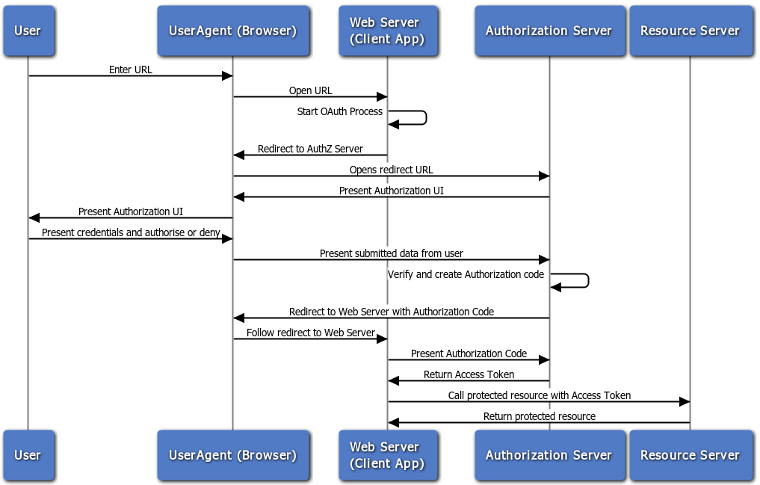
\includegraphics[width=0.95\linewidth]{images/web_flow.png}
    \caption{Diagrama que explica o funcionamento do fluxo de concessão do código de autorização, 
      definido na seção 4.1 da norma \emph{RFC 6749}. Fonte: \hyperref[link:oauth]{\emph{API Gateway OAuth 2.0 Authentication Flows}}.}%
    \label{fig:web_flow}
  \end{figure}
  

  \section{Integração e entrega contínua}
  Um dos grandes desafios no desenvolvimento de \emph{software} é criar um processo repetível e 
  confiável para entregas de aplicações. Frequentemente, lançamentos de \emph{software} são
  tratados por seus desenvolvedores como momentos estressantes. Associa-se este \emph{stress} a
  muitos processos manuais, infrequentes e propensos a erros, conduzidos em curtos prazos 
  de tempo.
  
  Pode-se, no entanto, se um processo rigoroso for seguido,  
  tornar esta tarefa fácil, tão fácil quanto o apertar de um botão.
  Para atingirmos este nível de maturidade no desenvolvimento de 
  \emph{software}, \citeonline{humble2010continuous} propõem que
  devemos seguir à risca dois princípios: automatização de todas etapas que sejam 
  automatizáveis e manter todos os artefatos necessários para um lançamento em um sistema de 
  controle de versões. 

  Idealmente, uma entrega de \emph{software} é composta por três atividades: 
  provisionar e gerenciar o ambiente em que a aplicação irá rodar (configuração de \emph{hardware},
  \emph{software}, infraestrutura e serviços externos), instalar a versão correta da aplicação 
  neste ambiente e configurar a aplicação, incluindo qualquer estado ou dado que ela possa requerer.

  De fato, até recentemente, vários destes passos para a entrega de \emph{software} pareciam 
  impossíveis ou ao menos complexas de aderirem os princípios citados por 
  \citeonline{humble2010continuous}. Como poderíamos, por exemplo, 
  versionar \emph{hardware}? Com o advento de virtualização eficiente e barata, até esta 
  tarefa que, \emph{a priori}, parecia impossível, virou algo corriqueiro e ubíquo. 
  Com advento e adoção da computação em nuvem, todos os passos necessários para automatização 
  de testes, compilação ou de artefatos e lançamento do \emph{software} estão 
  acessíveis a qualquer desenvolvedor.

  Define-se integração contínua como o processo no desenvolvimento de \emph{software} em que 
  membros de um time integram seu trabalho de forma frequente. Cada integração desencadeia etapas 
  como verificação de estilo de código, testes automatizados e construções de compilados ou 
  outros artefatos, com o objetivo de encontrar problemas nas integrações o mais rápido possível.
  Já entrega contínua leva a prática de integração contínua para outro patamar e automatiza 
  o lançamento de versões do \emph{software} dado que as etapas anteriores foram concluídas com 
  sucesso e o código foi revisado \cite{fowler2006continuous}.


\chapter{Desenvolvimento}
\label{chapter:desenvolvimento}
\section{Considerações Iniciais}
Este capítulo apresenta o projeto como um todo, explicando escolhas que foram 
feitas em seu desenvolvimento, tais como ferramentas e tecnologias adotadas. 
 


\section{Projeto}
Com o intuito de desenvolver um ambiente de ensino que fosse igualmente conveniente 
para professores estruturarem suas disciplinas de programação, 
tanto quanto agradável para alunos participarem de atividades, desenvolveu-se nesta monografia
 uma prova de conceito do que se envisinou poder ser esse sistema. Espera-se que, a partir 
 desta prova de conceito, atraía-se interessados pela construção de uma solução e 
 que, de forma coletiva, construa-se uma plataforma de excelência,
 por meio de colaborações em código aberto.

O professor na plataforma é capaz de criar e gerenciar exercícios, trilhas e turmas. 
Alunos se inscrevem na plataforma por meio de um \emph{login} de identidade federada, e 
ingressam nas turmas por meio de um \emph{link} específico, que é fornecido 
pelo professor nos primeiros dias de aula. 

Trilhas de exercícios são preparadas por professores, que a associam às suas turmas. 
Estas trilhas são compostas de Grupos de Exercícios Equivalentes que 
contêm exercícios de assuntos correlatos e, idealmente, de mesmo nível de dificuldade.
Para cada aluno, é sorteado um exercício de cada grupo de forma aleatória. 
Caso o aluno apresente dificuldade na resolução deste exercício, o aluno pode solicitar 
dicas relativas ao exercício, ou, em último caso, a solução do mesmo. Caso a solução 
seja requisitada, outro exercício do mesmo passo é sorteado a este aluno.

Para diminuir o escopo inicial do projeto e incentivar o estudante a se familiarizar com o ferramental 
que envolve desenvolvimento de software, escolheu-se que o desenvolvimento do código 
acontecesse localmente no computador do aluno. Para que, ainda sim, proporcionemos ao aluno 
uma boa experiência, desenvolveu-se uma interface por linha de comando, que nos referiremos a partir de agora 
por \emph{CLI} (\emph{Command Line Interface}). Por meio desta \emph{CLI},
o aluno pode fazer \emph{downloads} e submissões
dos exercícios propostos de maneira rápida e prática.

Dessa forma o sistema está dividido em três partes: uma interface gráfica, \emph{frontend}, 
em que professores e alunos possam interagir com exercícios, trilhas e turmas, uma \emph{CLI} que possibilita 
\emph{download} e submissão de exercícios, e um servidor com uma \emph{API} capaz de abstrair 
os recursos necessários por ambos os clientes. Na \fref{fig:arquitetura} apresenta-se um diagrama 
da arquitetura do sistema.

  \begin{figure}[htpb]
    \centering
    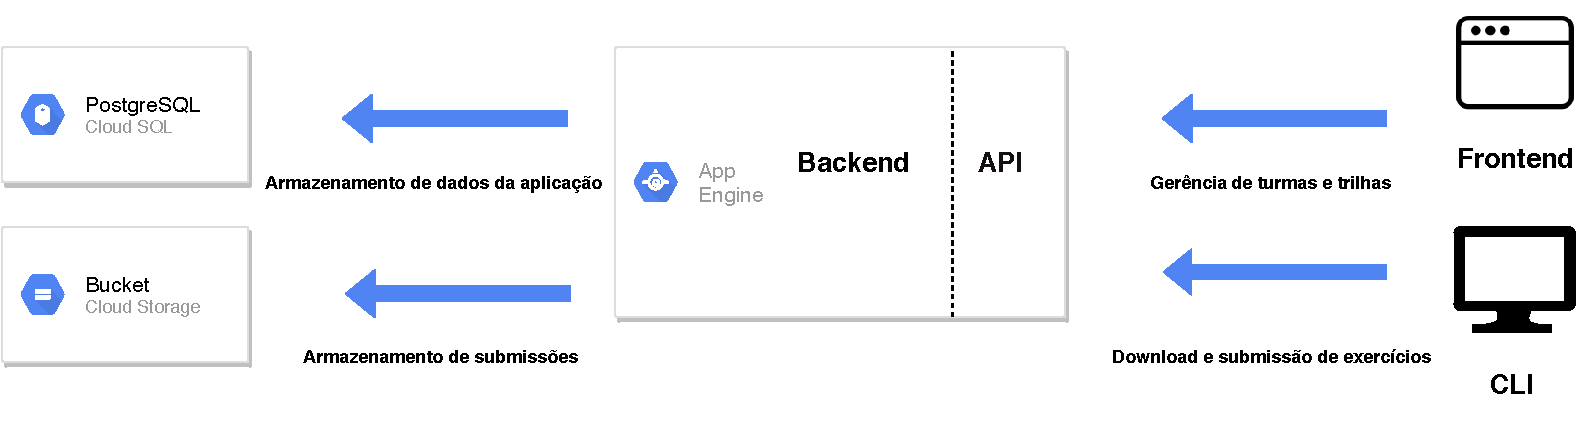
\includegraphics[width=\linewidth]{images/arquitetura.pdf}
    \caption{Diagrama que explica a arquietura do sistema \emph{Sharpener}, o qual 
    se desenvolveu uma prova de conceito.}%
    \label{fig:arquitetura}
  \end{figure}



\section{Atividades Realizadas}
\subsection{Desenvolvimento da \emph{API}}
Para o desenvolvimento da \emph{API}, escolheu-se a linguagem \emph{Python}, por sua clareza, 
e sua alta produtividade, que é crucial no processo de prototipação. Em conjunto com \emph{Python}, 
o \emph{micro framework web} \emph{Flask} também foi escolhido. Justifica-se essa escolha pela
inerente simplicidade, clareza e produtividade do \emph{framework}. 

Antes de podermos modelar recursos para a \emph{API},
estudou-se quais dados eram necessários para os casos de uso propostos. Este estudo gerou um 
\emph{MER}, modelo entidade relacional, que relacionava todas as entidades do sistema. A partir 
do diagrama gerado, criou-se ``\emph{models}'' que representavam estas entidades. A classe 
que possibilitou a criação destes \emph{models} provêm da \emph{ORM} que abstraí bancos 
relacionais chamada \hyperref[link:sqlalchemy]{\emph{SQLAlchemy}}. \hyperref[link:sqlalchemy]{\emph{SQLAlchemy}}
é uma biblioteca estável com mais de treze anos de maturidade,
mas que continua sendo a escolha padrão dos desenvolvedores.

Optou-se por utilizar \hyperref[link:postgresql]{\emph{PostgreSQL}}.
A escolha foi feita por se tratar de um sistema 
gerenciador de banco de dados relacional de código aberto e por este ser referência em 
desempenho e funcionalidades.

No mapeamento do \emph{MER}, previamente esboçado, em classes utilizou-se a biblioteca 
de visualização \hyperref[link:eralchemy]{\emph{ERAlchemy}}. \hyperref[link:eralchemy]{\emph{ERAlchemy}} é capaz de gerar 
diagramas \emph{MER} de forma automática a partir das classes modelo ou de uma conexão com o banco de dados. 
Tal ferramenta se provou excepcionalmente útil pois permitiu o desenvolvimento incremental e iterativo das 
classes modelo e garantiu que o modelo conceitual fosse implementado sem divergências. A \fref{fig:mer} mostra 
o modelo entidade relacional do sistema, gerado a partir da ferramenta.

Para que nosso sistema fosse capaz de armazenar submissões de alunos de forma confiável,  
um serviço de intervalos de  armazenamento, traduzido do inglês \emph{Bucket Storage}, se 
fez necessário. Um intervalo de armazenamento nada mais é que uma abstração de provedores 
de computação em nuvem para oferecer armazenamento de objetos. Uma das grandes vantagens associadas 
a este tipo de serviço é o baixo custo por \emph{gigabyte}, além de sua alta escalabilidade, tanto 
 um aumento no volume de dados armazenados, quanto na velocidade recuperação destes.
O provedor de computação em nuvem escolhido foi a \hyperref[link:gcp]{\emph{Google Cloud Plataform}}.


A alternativa a adotar um serviço de armazenamento por intervalos seria armazenar arquivos 
diretamente no banco de dados, o que traria um impacto na performance do mesmo, já que \emph{SGBD}s não são otimizados para
este tipo de dado. 

Modelou-se recursos seguindo o estilo arquitetural \emph{REST}. Coleções e documentos
de exercícios, turmas, tópicos, entre outros recursos foram implementados, e um 
recurso do arquétipo \emph{controller} foi necessário para prover autenticação a interface por 
meio do fluxo de concessão do código de autorização. Também disponibilizou-se uma rota para \emph{health check}, 
que permite que uma sonda externa consulte se a aplicação continua funcionando adequadamente. Caso esta não esteja, 
envia-se um sinal para que um novo container da aplicação seja iniciado e o tráfego é redirecionado a ela. 

Para que não seja necessário que professores criem um banco de exercícios do zero, um ``conector'' foi 
implementado para a plataforma \emph{exercism}, em que seus exercícios são extraídos e guardados no banco 
de dados. A implementação aborda apenas duas linguagens \emph{Python} e \emph{Rust}, mas 
pode ser facilmente estendido para outras linguagens, dado que se informe a estrutura de arquivos 
que os exercícios daquela linguagem são armazenados.

Também foi configurado uma plataforma de \emph{CI/CD} para o projeto. A toda nova versão enviada 
ao repositório remoto do sistema de controle de versões, uma tarefa rodava a ferramenta \emph{autopep8}
que checava se o código \emph{commitado} era sintaticamente válido e não seguia más práticas. 
Caso o código fosse reprovado na tarefa anterior, este não poderia ser aprovado e mesclado 
na \emph{branch} principal de desenvolvimento. Se a contribuição passar na verificação e 
depois de revisão for aceita, uma tarefa para lançamento da nova versão é disparada automaticamente, 
       que coloca uma nova versão no ar. A plataforma de \emph{CI/CD} empregada foi o 
       \hyperref[link:actions]{\emph{Github Actions}} e 
       as novas versões eram colocadas no ar através da \emph{Platform as a Service} do \emph{Google}, 
       \hyperref[link:appengine]{\emph{AppEngine}}.

\begin{sidewaysfigure}[htpb]
    \centering
    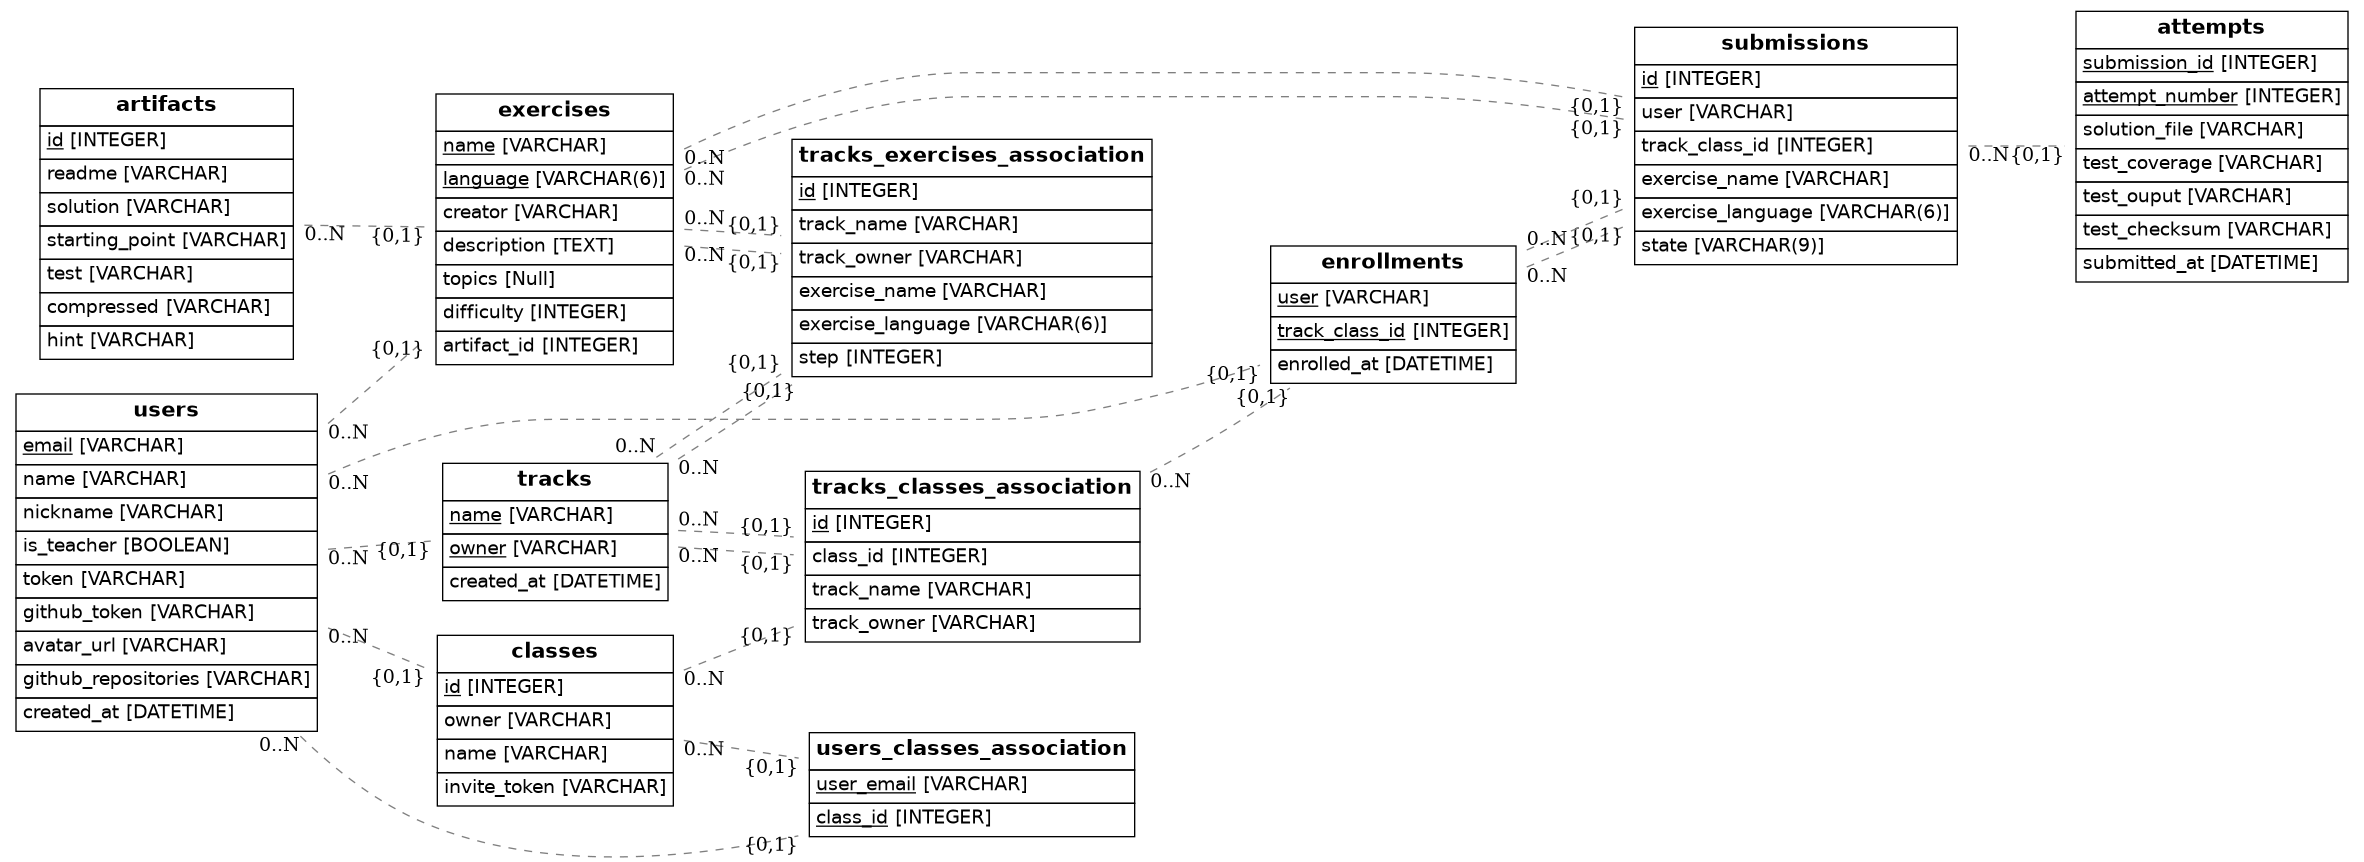
\includegraphics[width=\linewidth]{images/db_schema}
    \caption{Modelo entidade relacional gerado a partir da ferramenta \hyperref[link:eralchemy]{\emph{ERAlchemy}}.}\label{fig:mer}
\end{sidewaysfigure}


\subsection{Desenvolvimento da interface}
A interface foi desenvolvida utilizando \emph{Javascript}, \emph{CSS} e \emph{HTML}. Como 
desejávamos uma plataforma que fosse bastante interativa, uma \emph{single page application} 
foi implementada, utilizando a tecnologia \hyperref[link:react]{\emph{React}}.
Seguiu-se o \emph{design system} chamado 
\emph{Material Design} por ser bastante intuitivo para novos usuários. A biblioteca \emph{Material-UI} 
forneceu vários componentes que serviram de base para os componentes customizados. A comunicação com a 
\emph{API} foi feita utilizando o cliente \emph{HTTP} \hyperref[link:axios]{\emph{axios}} e 
os dados são persistidos numa \emph{store} local, utilizando o gerenciador de estados \emph{Redux}.


\subsection{Desenvolvimento da CLI}
O desenvolvimento da \emph{CLI} foi feito na linguagem \emph{Rust}, utilizando 
a biblioteca \emph{StructOpt}. \emph{StructOpt} é uma biblioteca que permite construção 
de interfaces por linhas de comando a partir da anotação de macros em \emph{structs} ou 
\emph{enums}. Com uma simples anotação ganha-se um \emph{parser} dos comandos e mensagens 
que instruem o usuário como utilizar sua \emph{CLI}.
 
 Aceitam-se três comandos na \emph{CLI}, ``\emph{download}'' que a partir de um identificador busca 
 o exercício proposto, \emph{submit} que manda uma tentiva de solução do problema ao servidor e 
 \emph{config}, necessário que seja executado, ao menos uma vez, com uma chave que identifica 
 qual aluno está utilizando o programa.

\section{Resultados}
A \fref{fig:login} mostra a página inicial da interface \emph{web} da ferramenta \emph{Sharpener}.
O \emph{login} do usuário é feito por contas previamente cadastradas na plataforma \emph{Github},
por meio fluxo de código de acesso. O professor quando logado, será direcionado a página 
de suas turmas, retratada na \fref{fig:turmas}, em que poderá gerenciá-las. Nesta página 
o professor também inscreve suas turmas em trilhas previamente criadas, como podemos 
observar em \fref{fig:enroll_track}. 

Pode-se acessar a página que possibilita a criação de trilhas 
através do menu lateral, que o leva a página retratada pela \fref{fig:track}. Nesta página 
pode-se criar novas trilhas como mostrado na \fref{fig:add_track1}. Uma trilha é composta por 
vários ``passos'', que são os \emph{clusters} de exercícios discutidos anteriormente. 
Ao clicar no botão de adicionar exercícios, surge um novo componente em que pode-se buscar 
e selecionar exercícios que farão parte daquele passo, conforme podemos observar em 
\fref{fig:add_track4}. Sabemos que a elaboração de exercícios é uma tarefa que toma 
muito tempo, portanto na página de exercícios, retratada pela \fref{fig:exercicios},
professores podem buscar por novos exercícios,  que foram criados por outros professores 
ou extraídos de alguma repositório público.


\section{Dificuldades e Limitações}
Encontraram-se duas grandes dificuldade na condução deste trabalho. 
A primeira delas foi a orquestração de diferentes tecnologias e partes do sistema. Houve um 
alto custo associado a dominar, utilizar e integrar diferentes linguagens, \emph{frameworks} 
e serviços. Ao longo do desenvolvimento deste projeto, percebeu-se que o escopo do projeto 
abordado foi inadequado para desenvolvimento no decorrer de um semestre.

Apesar, desde a concepção do projeto, o desenvolvimento proposto era de apenas uma prova 
de conceito de um sistema, esperava-se que, ao final da disciplina, um protótipo já adequado 
para testes em salas de aula fosse alcançado. Infelizmente, tal expectativa não foi cumprida.  
Apesar de uma parte significativa do sistema ter sido contemplada, ainda faltam 
muitas funcionalidades essenciais para que um ``teste de campo'' seja realizado.
% -> Login 
% -> Criação de turmas
% -> Criação de tracks
% -> Cluster de exercícios

  \begin{figure}[htpb]
    \centering
    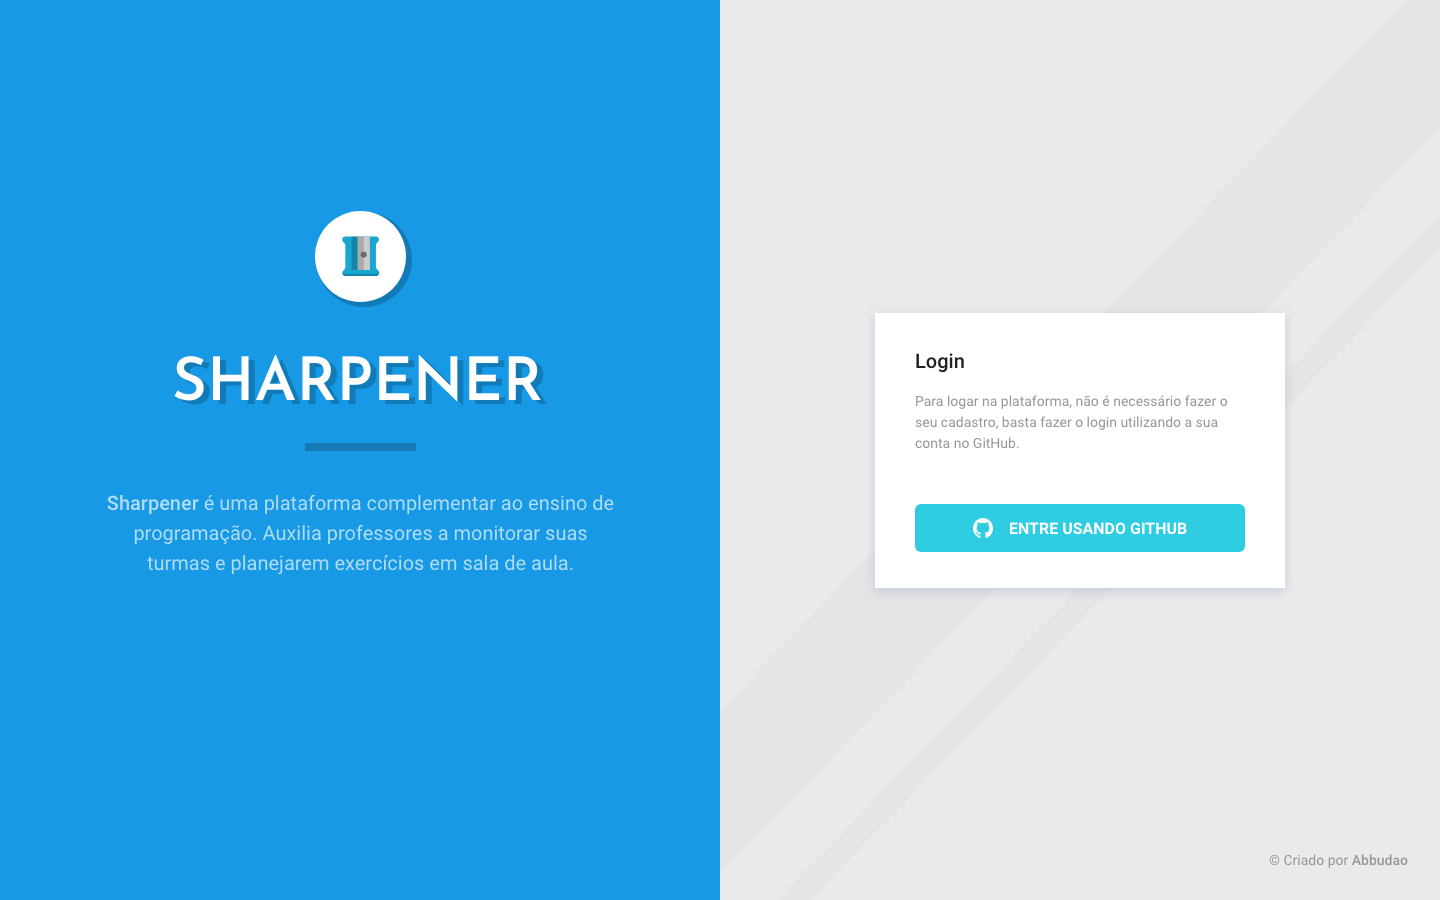
\includegraphics[width=\linewidth]{images/mocks/login.png}
    \caption{Página de \emph{Login} da prova de conceito do sistema \emph{Sharpener}.}%
    \label{fig:login}
  \end{figure}

  \begin{figure}[htpb]
    \centering
    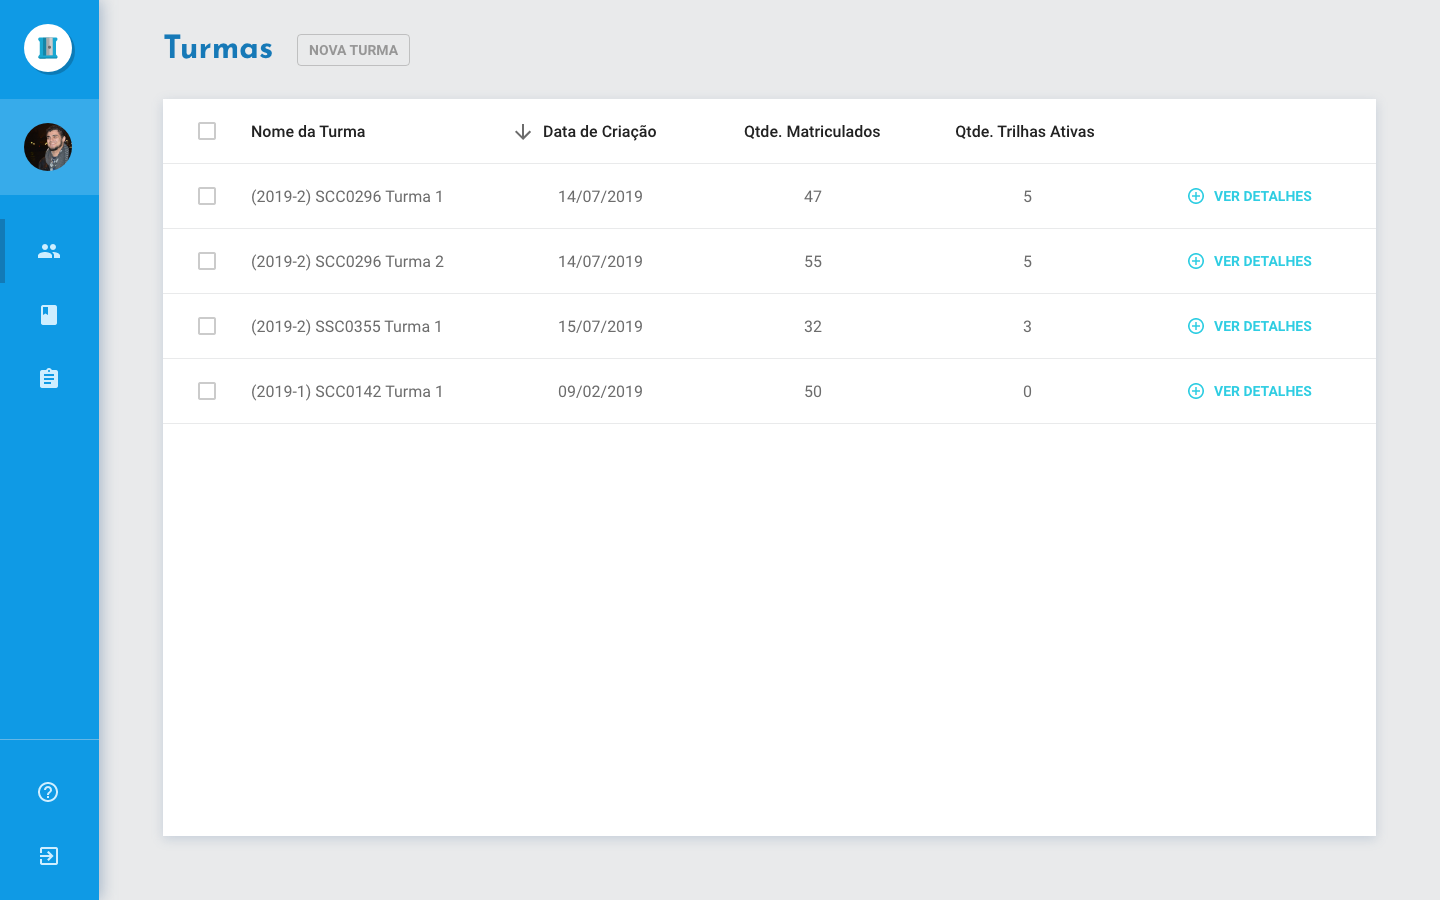
\includegraphics[width=\linewidth]{images/mocks/turma.png}
    \caption{Página de turmas da prova de conceito do sistema \emph{Sharpener}.}%
    \label{fig:turmas}
  \end{figure}

  \begin{figure}[htpb]
    \centering
    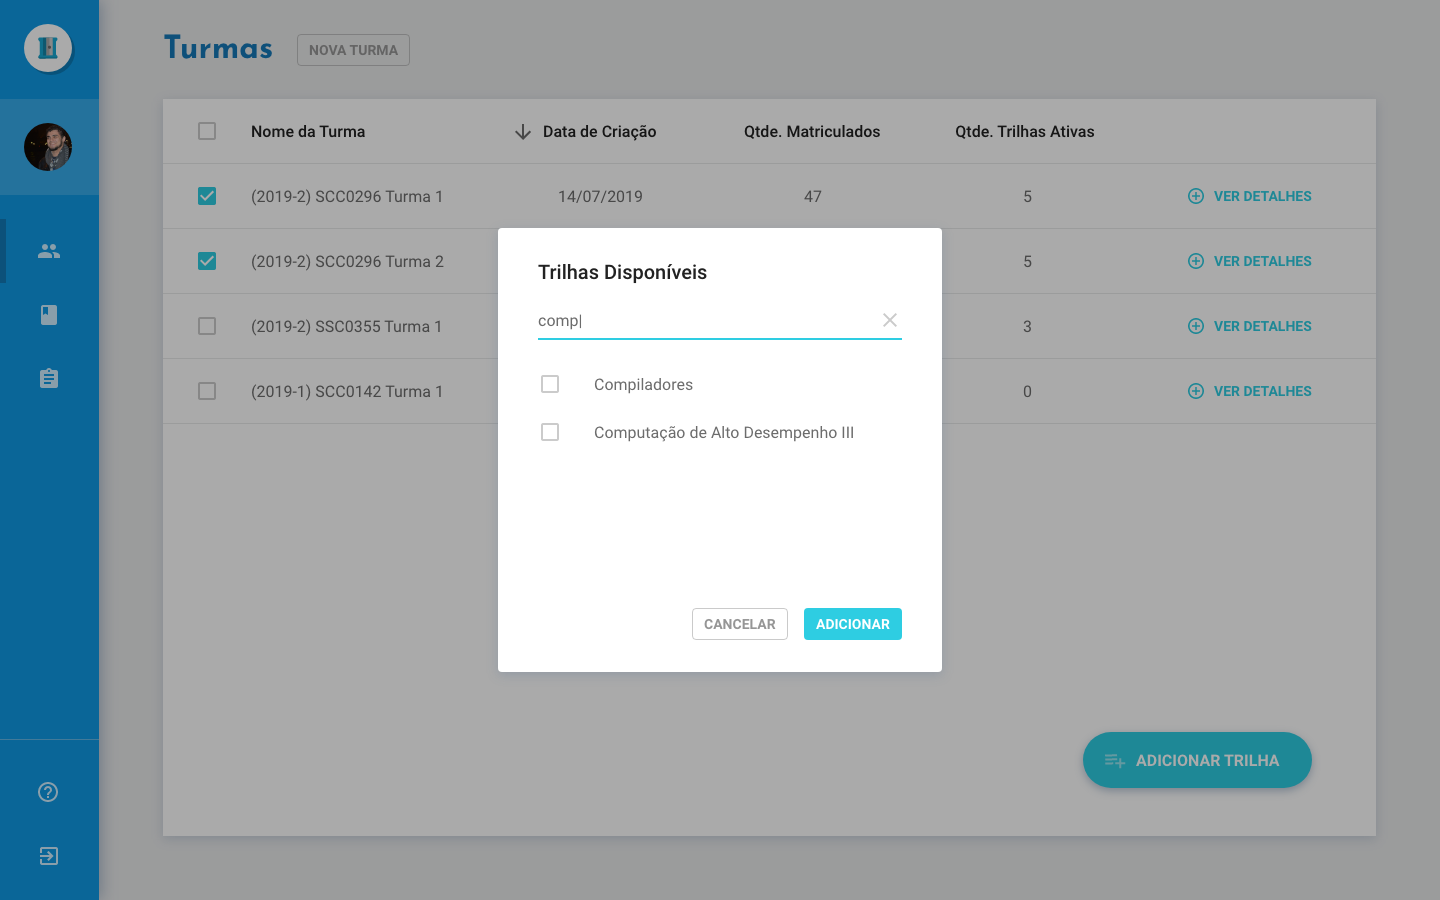
\includegraphics[width=\linewidth]{images/mocks/turmaAddTrackSearch.png}
    \caption{Página de turmas da prova de conceito do sistema \emph{Sharpener}, em 
	    que o professor inscreve suas turmas em trilhas.}%
    \label{fig:enroll_track}
  \end{figure}

  \begin{figure}[htpb]
  \centering
  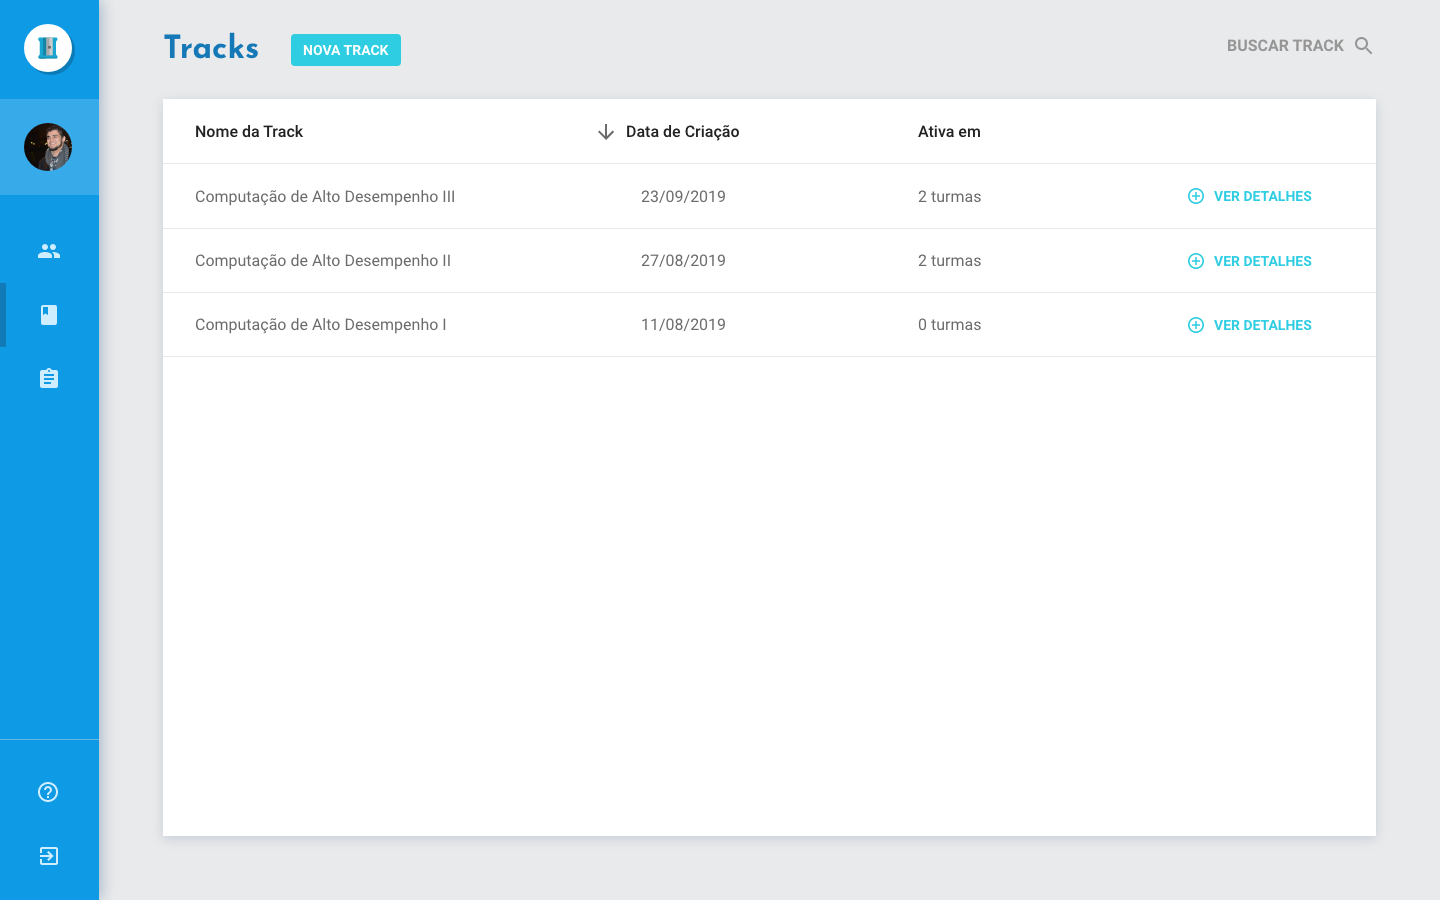
\includegraphics[width=\linewidth]{images/mocks/track.png}
  \caption{Página de trilhas da prova de conceito do sistema \emph{Sharpener}.}%
  \label{fig:track}
  \end{figure}

  \begin{figure}[htpb]
  \centering
  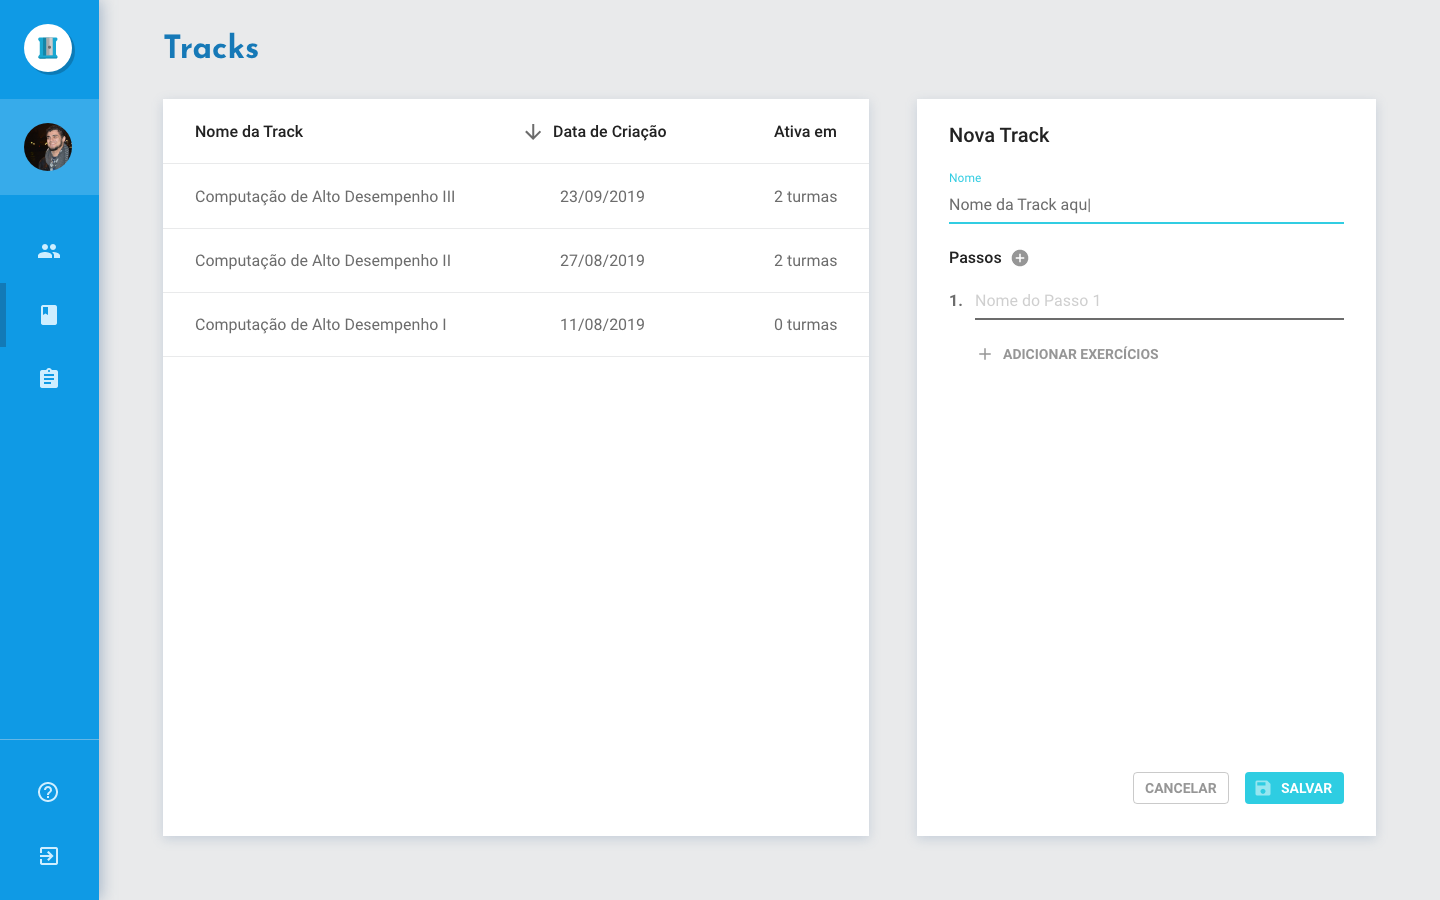
\includegraphics[width=\linewidth]{images/mocks/trackAdd1.png}
  \caption{Página de trilhas da prova de conceito do sistema \emph{Sharpener}, 
  em que uma nova trilha é criada.}%
  \label{fig:add_track1}
  \end{figure}

  \begin{figure}[htpb]
  \centering
  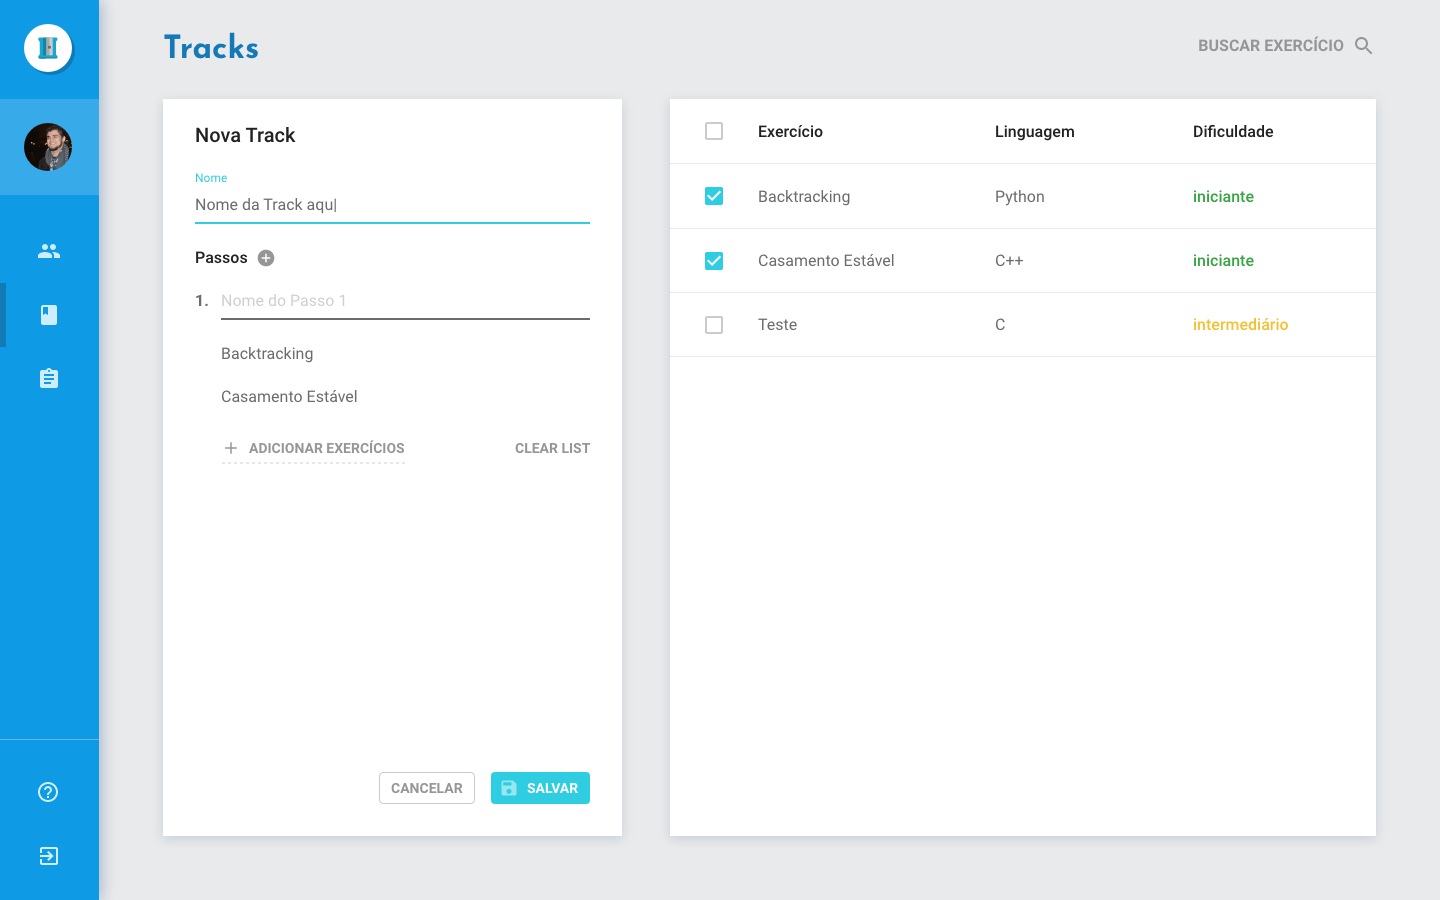
\includegraphics[width=\linewidth]{images/mocks/trackAdd4.png}
  \caption{Página de trilhas da prova de conceito do sistema \emph{Sharpener}, 
	  em que \emph{clusters de exercícios} são associados a passos de uma trilha.}%
  \label{fig:add_track4}
  \end{figure}

\begin{figure}[htpb]
  \centering
  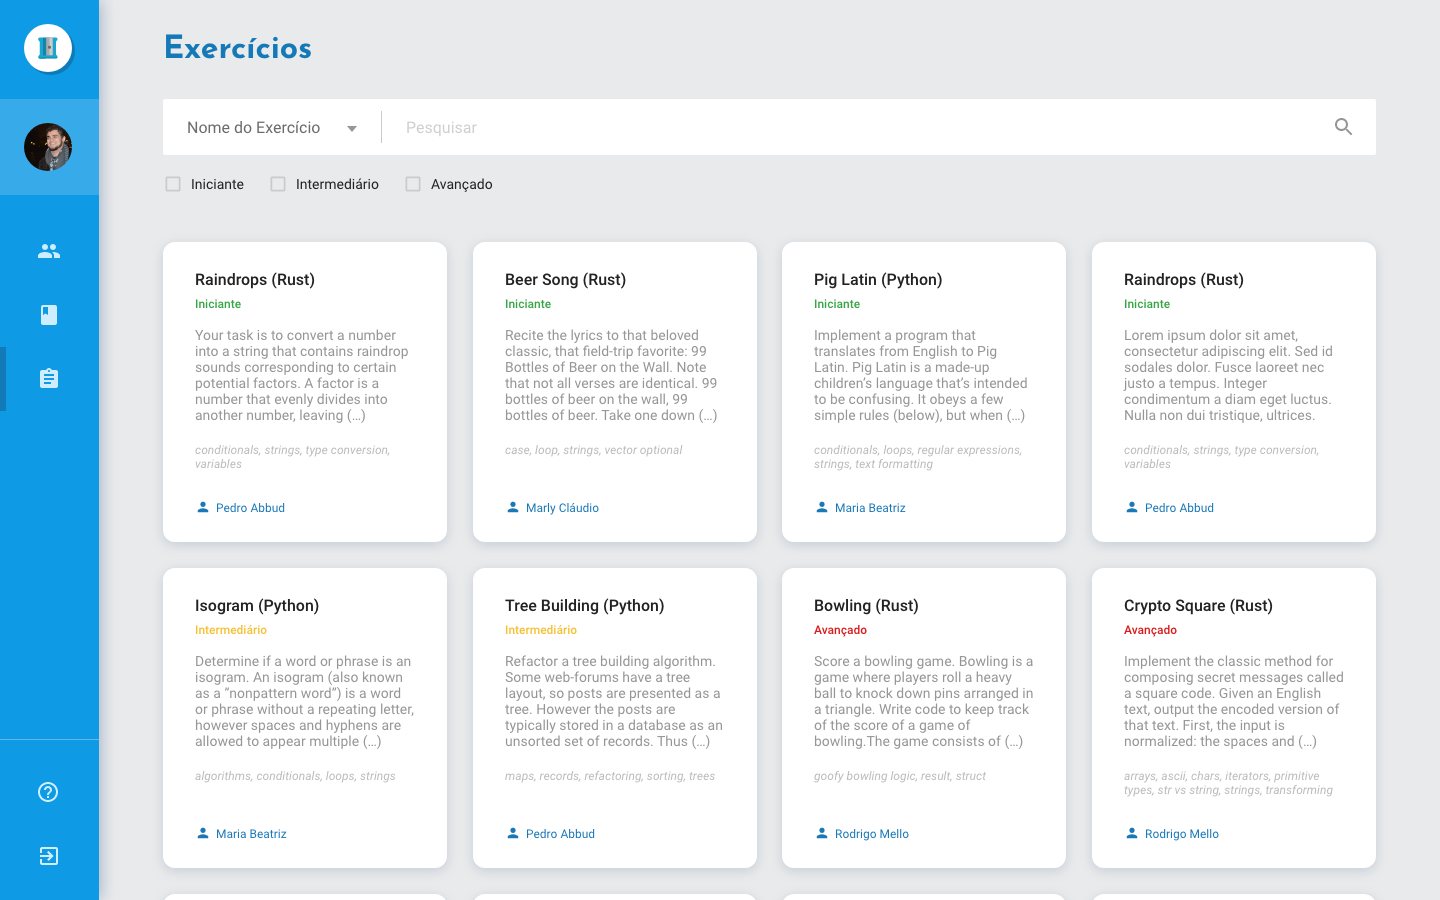
\includegraphics[width=\linewidth]{images/mocks/exercicios.png}
  \caption{Página de exercícios da prova de conceito do sistema \emph{Sharpener}.}%
  \label{fig:exercicios}
  \end{figure}


\chapter{Desenvolvimento 2.0}
\label{chapter:desenvolvimento2}
\label{chapter:desenvolvimento}
\section{Considerações Iniciais}
Neste capítulo expressa-se como foi vislumbrado um sistema de apoio didático ao ensino de programação, de que maneira foi modelado, 
quais decisões arquiteturais foram tomadas e como foi realizada sua implementação. Apresenta-se aqui uma visão geral do sistema, a visão específica que cada ator tem do sistema e a jornada de cada um desses usuários. De forma resumida, também é discutida a implementação das partes que compõem o sistema.
\section{Visão Geral}
O sistema \emph{Sharpener} foi construído para interagir com dois tipos de usuários; o Aluno e o Professor. O Professor pretende utilizar o \emph{Sharpener}
 em sala de aula, pois se interessa em ferramentas de apoio ao ensino e gostaria de acompanhar mais de perto a parte prática de suas aulas. O Aluno 
gostaria de utilizar ferramentas cômodas que o ajudassem no entendimento e resolução de exercícios.
% Quem são os atores do sistema? R: Professor e aluno

% Quais são os objetivos do professor no sistema? recuperar o plano 
% no Google Docs como redação (menos as partes que desistimos de fazer
Do ponto de vista do Professor, a ferramenta traz: a criação de um banco de exercícios, organizados por tópicos, 
de forma compartilhada entre professores; a possibilidade de inserção de dicas para auxiliar na resolução de exercícios; 
a possibilidade da elaboração de exercícios incrementais e um melhor acompanhamento do aluno levando em conta quais exercícios teve dificuldade. 
Do ponto de vista do Aluno, a ferramenta traz:  acesso a dicas, a opção de visualização da resposta do exercício e a substituição por exercício equivalente;
acesso a exercícios incrementais e uma forma 
simplificada de acesso e submissão de exercícios.

% Quais são os objetivos do aluno no sistema?
% recuperar plano, idem
O professor na plataforma é capaz de criar e gerenciar exercícios, trilhas e turmas. 
Alunos se inscrevem na plataforma por meio de um \emph{login} de identidade federada, e 
ingressam nas turmas por meio de um \emph{link} específico, que é fornecido 
pelo professor nos primeiros dias de aula. 

Trilhas de exercícios são preparadas por professores, que a associam às suas turmas. 
Estas trilhas são compostas de Grupos de Exercícios Equivalentes que 
contêm exercícios de assuntos correlatos e, idealmente, de mesmo nível de dificuldade.
Para cada aluno, é sorteado um exercício de cada grupo de forma aleatória. 
Caso o aluno apresente dificuldade na resolução deste exercício, o aluno pode solicitar 
dicas relativas ao exercício, ou, em último caso, a solução do mesmo. Caso a solução 
seja requisitada, outro exercício do mesmo Grupo de Exercícios Equivalentes é sorteado a este aluno.

Para diminuir o escopo inicial do projeto e incentivar o estudante a se familiarizar com o ferramental 
que envolve desenvolvimento de software, escolheu-se que o desenvolvimento do código 
acontecesse localmente no computador do aluno. Para que, ainda assim, proporcionemos ao aluno 
uma boa usabilidade do sistema, desenvolveu-se uma interface por linha de comando, que nos referiremos a partir de agora 
por \emph{CLI} (\emph{Command Line Interface}). Por meio desta \emph{CLI},
o aluno pode fazer \emph{downloads} e submissões
dos exercícios propostos de maneira rápida e prática.

Dessa forma, o sistema está dividido em três partes: uma interface gráfica, \emph{frontend}, 
em que professores e alunos possam interagir com exercícios, trilhas e turmas, uma \emph{CLI} que possibilita 
\emph{download} e submissão de exercícios, e um servidor com uma \emph{API} capaz de abstrair 
os recursos necessários por ambos os clientes. 

Na \fref{fig:arquitetura} apresenta-se um diagrama 
da arquitetura do sistema. Tanto a \emph{CLI} quanto o \emph{Frontend} se comunicam com o servidor através de sua \emph{API} \emph{Web} para que possa cumprir suas funcionalidades. A \emph{API} dispara funções no \emph{Backend} para que o recurso requisitado seja salvo ou recuperado. A maior parte dos dados do \emph{Backend} vem de uma conexão com o banco \emph{PostgreSQL}, hospedado no serviço \emph{Cloud SQL}. Apenas arquivos são salvos e recuperados através de requisições ao intervalo de armazenamento, chamado de \emph{Bucket}. 

  \begin{figure}[htpb]
    \centering
    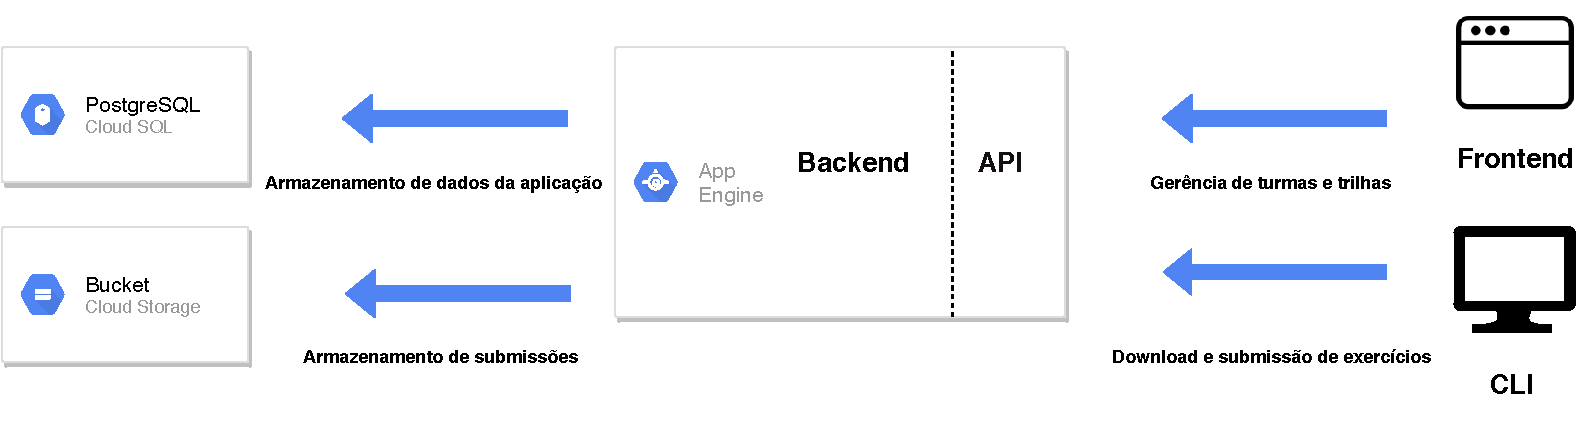
\includegraphics[width=\linewidth]{images/arquitetura.pdf}
    \caption{Arquitetura do sistema \emph{Sharpener}, o qual 
    se desenvolveu uma prova de conceito.}%
    \label{fig:arquitetura}
  \end{figure}
% Arquitetura resumida: a figura que já está pronta e o texto lá.

% Implementação, um resumo das linguagens e ferramentas 

\section{O sistema do ponto de vista do Aluno}
\label{ssec:aluno}

A rotina do Aluno no \emph{Sharpener} consiste em: ter acesso a um exercício, recorrer a alguma forma de apoio, completar o exercício submetendo uma versão, obter \emph{feedback}, e acompanhar seu andamento no curso. As principais atividades são realizadas na \emph{CLI}.

\subsection{Configuração}


O aluno tem acesso a uma interface de linha de comando, 
disponível para \emph{download} no \emph{Frontend}. Em seu primeiro 
acesso, o Aluno deve declarar que é o dono de uma \emph{token} que o identifica, isto é feito através do comando descrito em \cref{codigo:config}. A \emph{token} é obtida no \emph{Frontend}, depois de realizado o primeiro \emph{login}.

O aluno também deve ingressar na turma referente a seu professor, através de um \emph{link}, único para cada turma,
que será disponibilizado em sala de aula.

\begin{codigo}[caption={Configuração da CLI.}, label={codigo:config},language=bash, breaklines=true]
student@usp:~$ sharpener config <identificador-aluno>
\end{codigo}


\subsection{Acesso a exercícios}
Com a \emph{CLI} configurada, o aluno pode consultar 
se existem submissões pendentes. Para isto, deve recorrer ao 
comando descrito no \cref{codigo:list}. O comando invoca uma lista com todas as próximas submissões pendentes das trilhas em que está inscrito. Na listagem, cada submissão apresenta um identificador único.

\begin{codigo}[caption={Comando que lista submissões pendentes.}, label={codigo:list},language=bash, breaklines=true]
student@usp:~$ sharpener list
\end{codigo}

Com o identificador de submissão em mãos, o comando descrito em \cref{codigo:download} é utilizado para criar 
uma pasta com o nome do exercício no diretório que o comando foi invocado. Na pasta, todos os 
arquivos necessários para o desenvolvimento de uma solução estão presentes: descrição detalhada 
do problema, testes, um arquivo especificando dependências e um ponto de entrada.
Cada linguagem apresenta uma estrutura diferente de pastas, o \cref{codigo:pasta} mostra a execução 
do comando ``\emph{tree}'' que mostra como é a organização dos arquivos para a linguagem \emph{Rust}, no exercício \emph{accumulate}.
O aluno deve desenvolver sua solução no arquivo de ponto de entrada, 
que no exemplo anterior, se encontra em ``src/lib.rs''.

\begin{codigo}[caption={Download de exercício pela \emph{CLI}.}, label={codigo:download},language=bash, breaklines=true]
student@usp:~$ sharpener download <identificador-exercicio>
\end{codigo}

\newpage
\begin{codigo}[caption = {Estrutura de pasta para um exercício em Rust}, label={codigo:pasta},language=bash, breaklines=true]
student@usp~$ tree
    Cargo.toml
    README.md
    src
        lib.rs
    tests
        accumulate.rs
2 directories, 5 files

\end{codigo}

% explicar a consulta na CLI (não existe, vamos desenhar/projetar)
% explicar o download na CLI

\subsection{Apoio a resolução de exercício}
Para que o aluno consiga evoluir sua solução até uma que esteja correta, testes automatizados estão presentes 
nos exercícios disponíveis no \emph{Sharpener}. Com o comando descrito em \cref{codigo:test}, os testes são 
executados e impressos no terminal. Caso todos os testes forem cumpridos, o código está pronto para submissão, do contrário 
mudanças devem ser feitas no código e repete-se o processo.

\begin{codigo}[caption = {Executando a bateria de testes a partir da \emph{CLI}.}, label={codigo:test},language=bash, breaklines=true]
student@usp:~$ sharpener test 
\end{codigo}

% Buscando dicas
Caso o professor deseje disponibilizar dicas acerca do exercício, o Aluno pode invocar o comando descrito no \cref{codigo:hint}. 
Uma nova dica será mostrada no terminal, guiando o Aluno na resolução do exercício.

\newpage
\begin{codigo}[caption = {Comando para solicitar dicas do exercício na \emph{CLI}.}, label={codigo:hint},language=bash, breaklines=true]
student@usp:~$ sharpener hint
\end{codigo}

% Buscando/obtendo a resposta final
O Aluno, em último caso, pode desistir de resolver aquele exercício em específico do Grupo de Exercícios Equivalentes. 
O comando descrito em \cref{codigo:solution}, após uma confirmação do aluno, faz \emph{download} de um arquivo contendo uma possível 
solução. Quando o comando é emitido, é registrado que aquele exercício do Grupo de Exercícios Equivalentes foi pulado e um novo exercício é 
baixado e colocado no diretório pai do exercício atual. A desistência só é possível se houver outro exercício disponível no Grupo de Exercício Equivalentes.

Para que a submissão seja válida o arquivo de testes deverá ser idêntico ao que foi baixado. Caso 
este contenha modificações, a \emph{CLI} notificará o aluno que este é o caso e abortará a submissão.
\begin{codigo}[caption = {Comando para requisitar a solução de um exercício na \emph{CLI}}, label={codigo:solution},language=bash, breaklines=true]
student@usp:~$ sharpener solution
\end{codigo}



% Buscando/obtendo um Exercício Equivalente/Alternativo

\subsection{Submissão de resposta}
% 
Se a solução desenvolvida pelo Aluno cumprir todos os testes, sua submissão é possível. Com o comando descrito por \cref{codigo:submit}, 
sua solução é enviada, juntamente com o \emph{output} dos testes. Caso o comando seja invocado e os testes ainda não estão sendo cumpridos, um 
alerta notifica o Aluno que este é o caso, e o questiona se deseja continuar mesmo assim. Múltiplas tentativas de submissão podem ser feitas, 
sendo todas elas salvas pelo sistema. Assume-se que a última submissão é a que deve ser corrigida, mas o professor, se desejar, pode inspecionar tentativas feitas anteriormente.

\begin{codigo}[caption = {Comando para submeter exercícios na \emph{CLI}}, label={codigo:submit},language=bash, breaklines=true]
student@usp:~$ sharpener submit
\end{codigo}

%\subsection{Exercícios incrementais}

%\subsection{Acompanhamento do andamento na disciplina}

\section{O sistema do ponto de vista do Professor} 
\label{ssec:professor}
\subsection{Gerenciando turmas e trilhas}
A jornada do professor também começa no \emph{Frontend}, que tem sua página inicial descrita pela \fref{fig:login}.
Após seu \emph{login} pelo \emph{Github}, este deve informar a um administrador 
do sistema que sua conta precisa ser elevada a condição de professor, já que todas as contas são alunos por \emph{default}.

  \begin{figure}[htb]
    \centering
    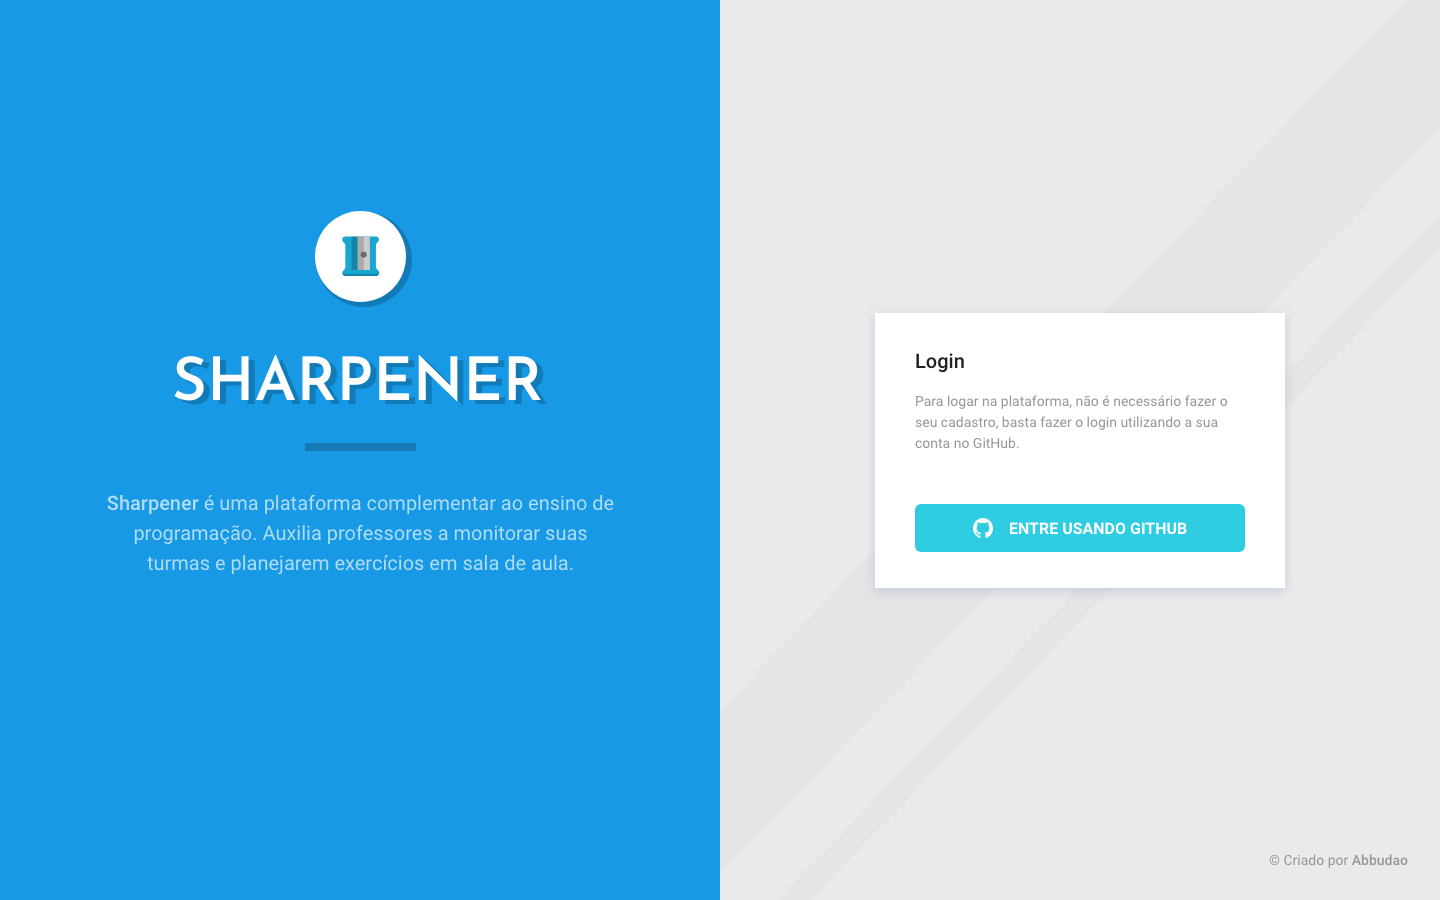
\includegraphics[width=\linewidth]{images/mocks/login.png}
    \caption{Página de \emph{Login} da prova de conceito do sistema \emph{Sharpener}.}%
    \label{fig:login}
  \end{figure}

Assim que o Professor fizer \emph{login} na plataforma, o Professor é direcionado para página de turmas, como podemos visualizar na \fref{fig:turmas}. 
Este deve criar sua primeira turma, dando a ela um nome único, como mostra a \fref{fig:turmasAdd}. 

 \begin{figure}[htpb]
    \centering
    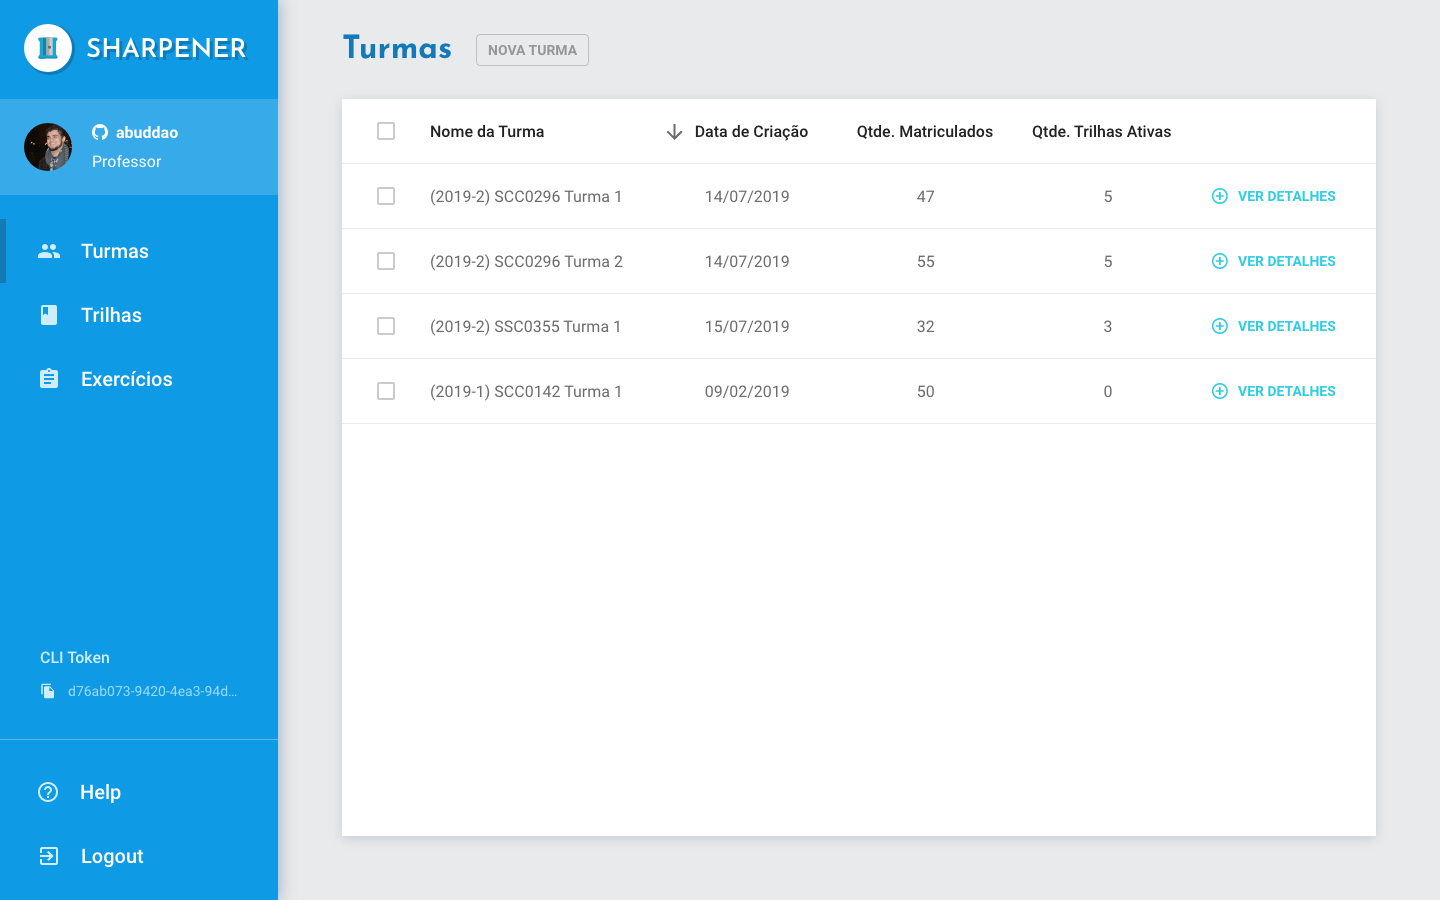
\includegraphics[width=\linewidth]{images/mocks/turmaExpandido.png}
    \caption{Página de turmas da prova de conceito do sistema \emph{Sharpener}.}%
    \label{fig:turmas}
  \end{figure}
  
    \begin{figure}[htpb]
    \centering
    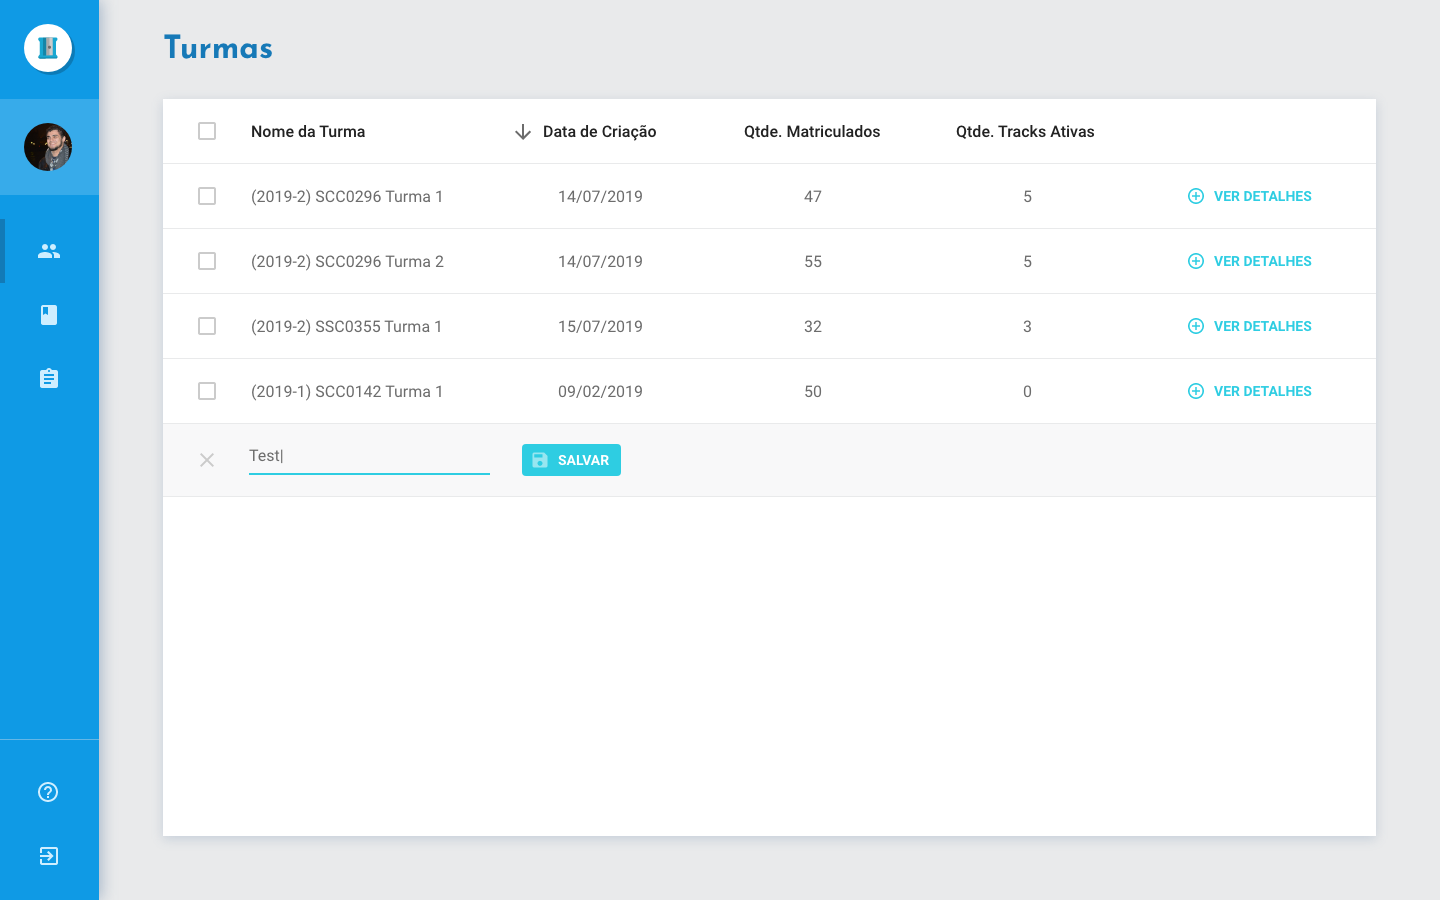
\includegraphics[width=\linewidth]{images/mocks/turmaNova.png}
    \caption{Página de turmas da prova de conceito do sistema \emph{Sharpener}, em que se 
    cria uma nova turma.}%
    \label{fig:turmasAdd}
  \end{figure}

O próximo passo é a criação de uma trilha de exercícios, que pode ser feita na página descrita pela \fref{fig:track}. Cada trilha
contém Grupos de Exercícios Equivalentes. O professor associa exercícios 
a cada um destes grupos, podendo filtrá-los por nome na barra superior direto. 
Tal sequência é mostrada pela \fref{fig:add_track1}, \fref{fig:add_track2}, \fref{fig:add_track3} e \fref{fig:add_track4}.  

  \begin{figure}[htb]
  \centering
  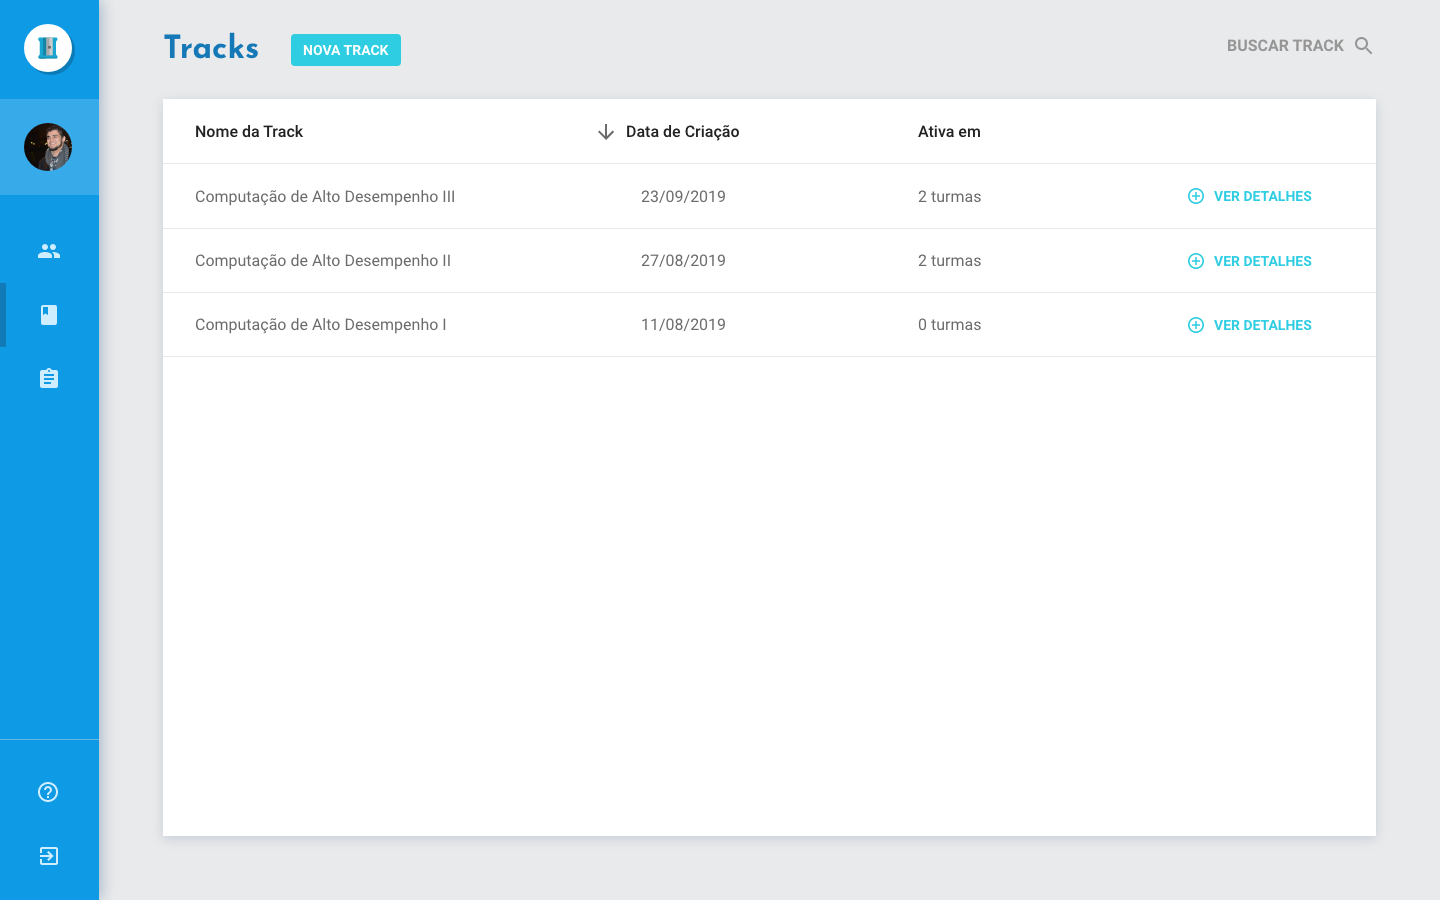
\includegraphics[width=\linewidth]{images/mocks/track.png}
  \caption{Página de trilhas da prova de conceito do sistema \emph{Sharpener}.}%
  \label{fig:track}
  \end{figure}
  
    \begin{figure}[htpb]
  \centering
  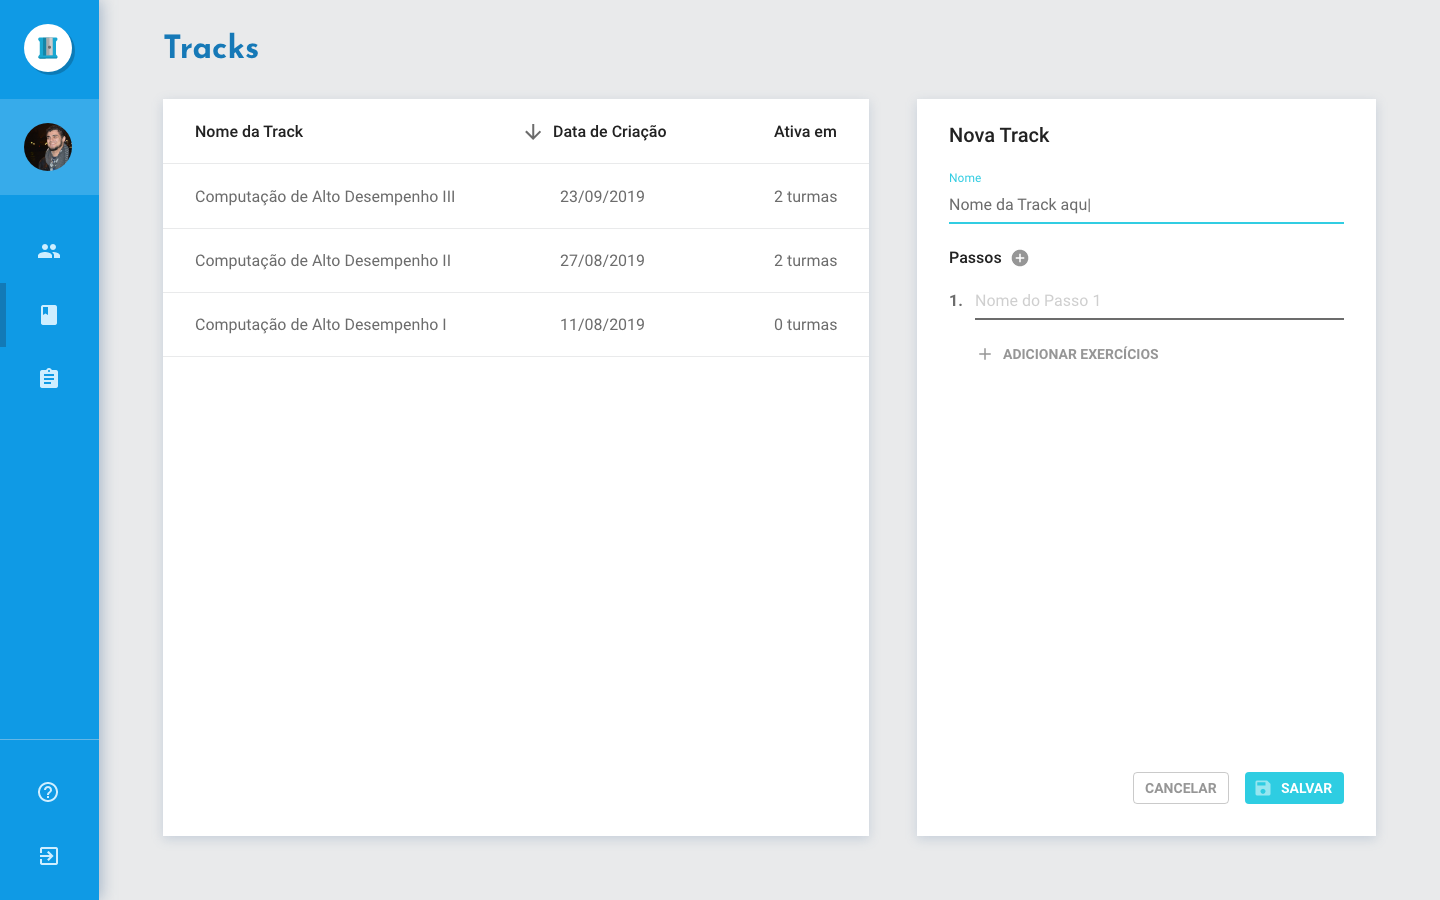
\includegraphics[width=\linewidth]{images/mocks/trackAdd1.png}
  \caption{Página de trilhas da prova de conceito do sistema \emph{Sharpener}, 
  em que uma nova trilha é criada.}%
  \label{fig:add_track1}
  \end{figure}
  
    \begin{figure}[htpb]
  \centering
  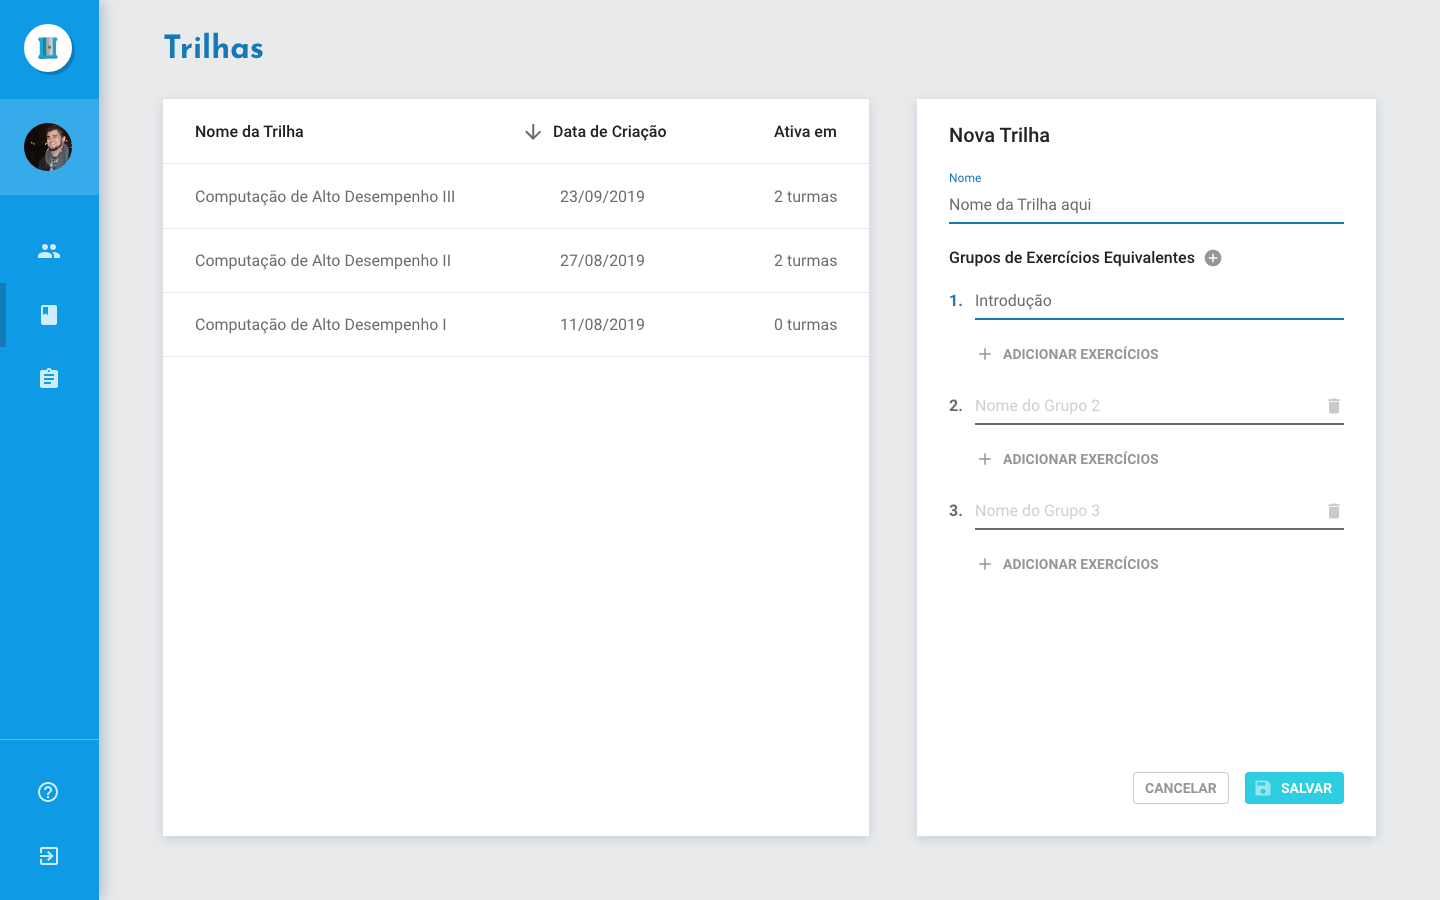
\includegraphics[width=\linewidth]{images/mocks/trackAdd2.png}
  \caption{Página de trilhas da prova de conceito do sistema \emph{Sharpener}, 
  em que novos Grupos de Exercícios Equivalentes são criados.}%
  \label{fig:add_track2}
  \end{figure}

  \begin{figure}[htpb]
  \centering
  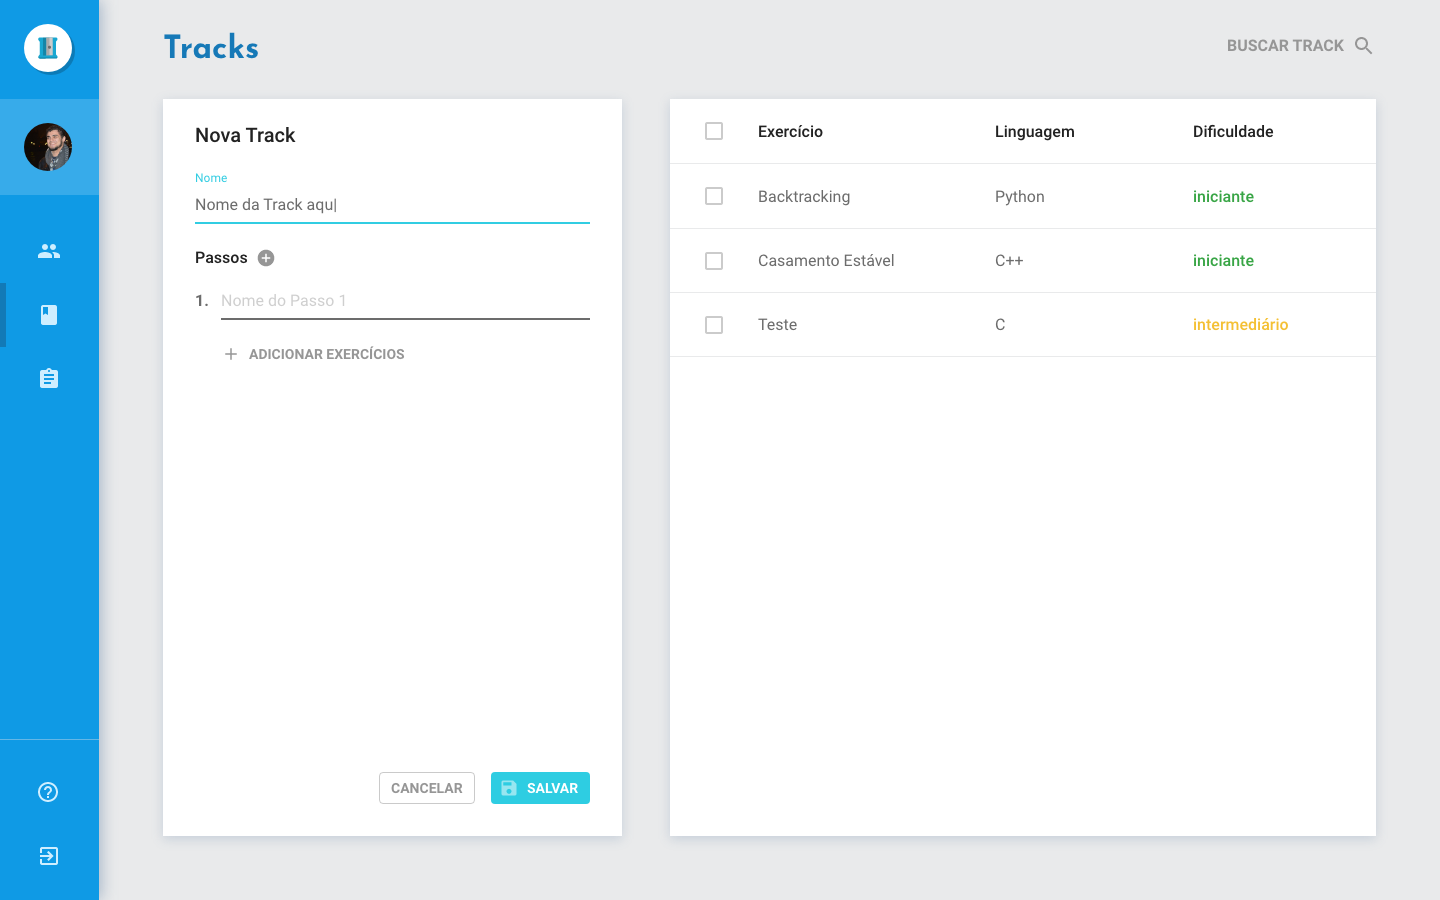
\includegraphics[width=\linewidth]{images/mocks/trackAdd3.png}
  \caption{Página de trilhas da prova de conceito do sistema \emph{Sharpener}, 
	  em que Grupos de Exercícios Equivalentes são associados a passos de uma trilha, parte 1.}%
  \label{fig:add_track3}
  \end{figure}
  
  \begin{figure}[htpb]
  \centering
  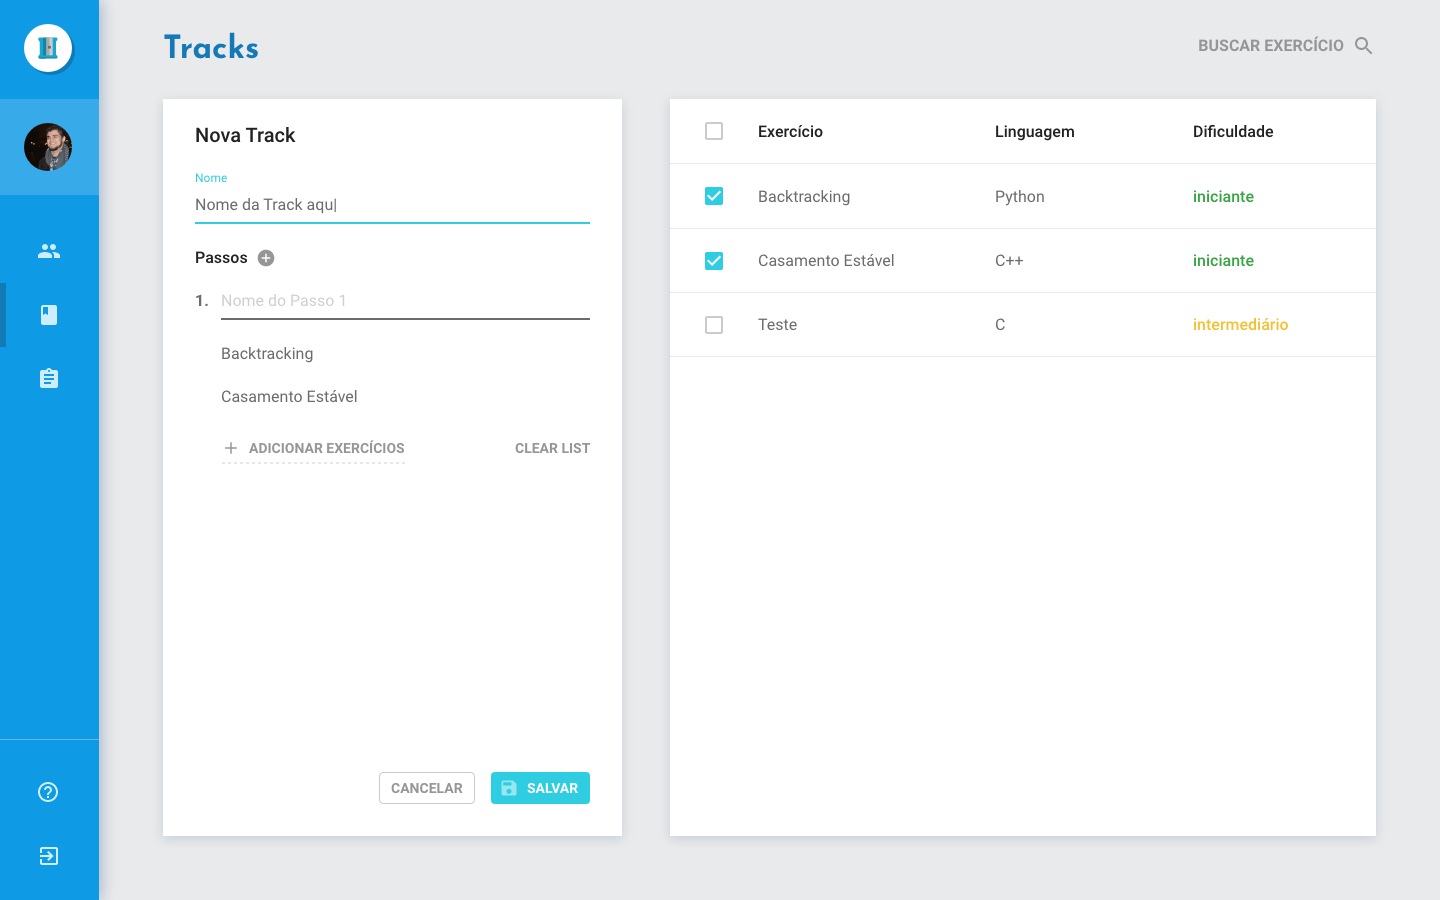
\includegraphics[width=\linewidth]{images/mocks/trackAdd4.png}
  \caption{Página de trilhas da prova de conceito do sistema \emph{Sharpener}, 
	  em que Grupos de Exercícios Equivalentes são associados a passos de uma trilha, parte 2.}%
  \label{fig:add_track4}
  \end{figure}

Caso o professor ainda não tenha definido todos os exercícios que compõem sua trilha, uma visita a página de exercícios pode lhe 
ser útil. A página conta com todos os exercícios disponíveis no banco de exercícios que podem ser filtrados por nomes ou tópicos, 
como pode ser visto pela \fref{fig:exercicios}.

  \begin{figure}[htb]
  \centering
  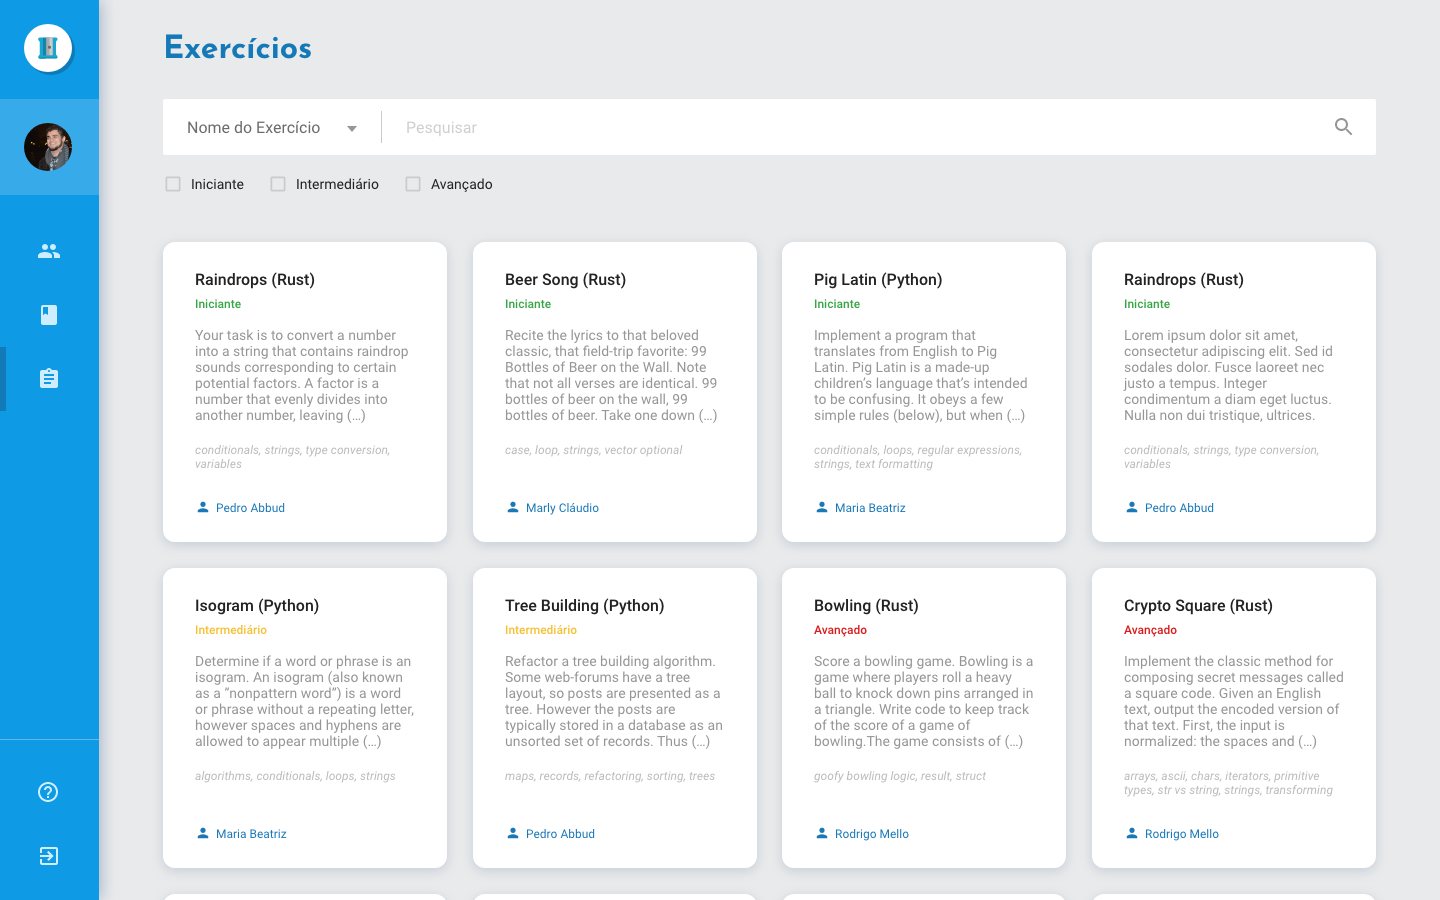
\includegraphics[width=\linewidth]{images/mocks/exercicios.png}
  \caption{Página de exercícios da prova de conceito do sistema \emph{Sharpener}.}%
  \label{fig:exercicios}
  \end{figure}

O passo final é associar a trilha recém criada às suas turmas. Isto pode ser feito voltando na página de turmas, selecionando 
turmas e clicando no botão ``Adicionar \emph{Track}''. Um modal cobre a tela e é possível selecionar e procurar trilhas, dentre 
as disponíveis, para associar a estas turmas. A \fref{fig:enroll_track1} e \fref{fig:enroll_track2} mostram esta interação.

  \begin{figure}[htb]
    \centering
    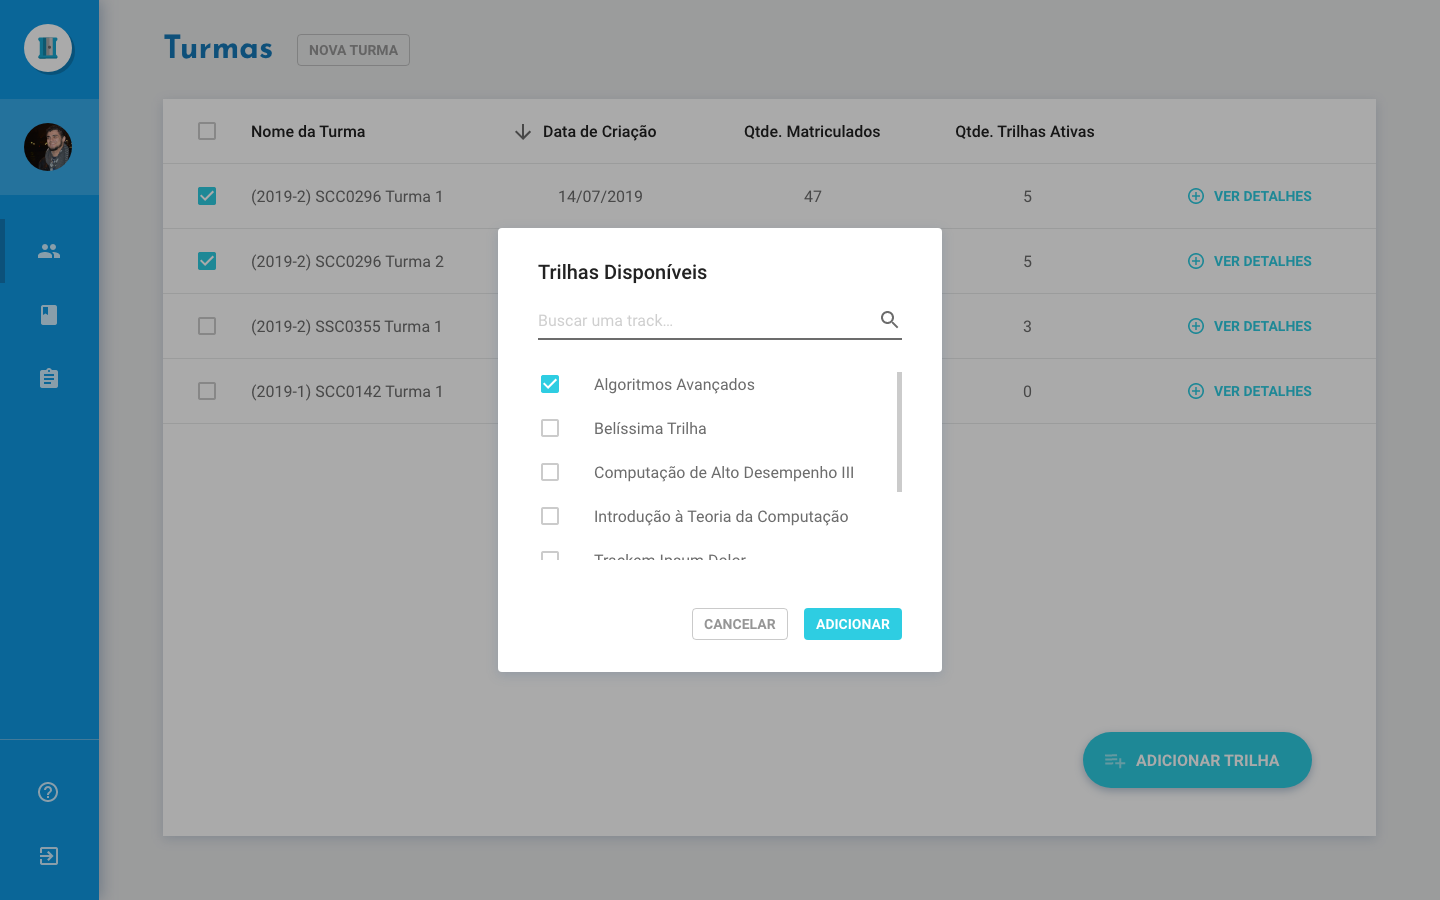
\includegraphics[width=\linewidth]{images/mocks/turmaAddTrack.png}
    \caption{Página de turmas da prova de conceito do sistema \emph{Sharpener}, em 
	    que o professor inscreve suas turmas em trilhas.}%
    \label{fig:enroll_track1}
  \end{figure}
  
    \begin{figure}[htb]
    \centering
    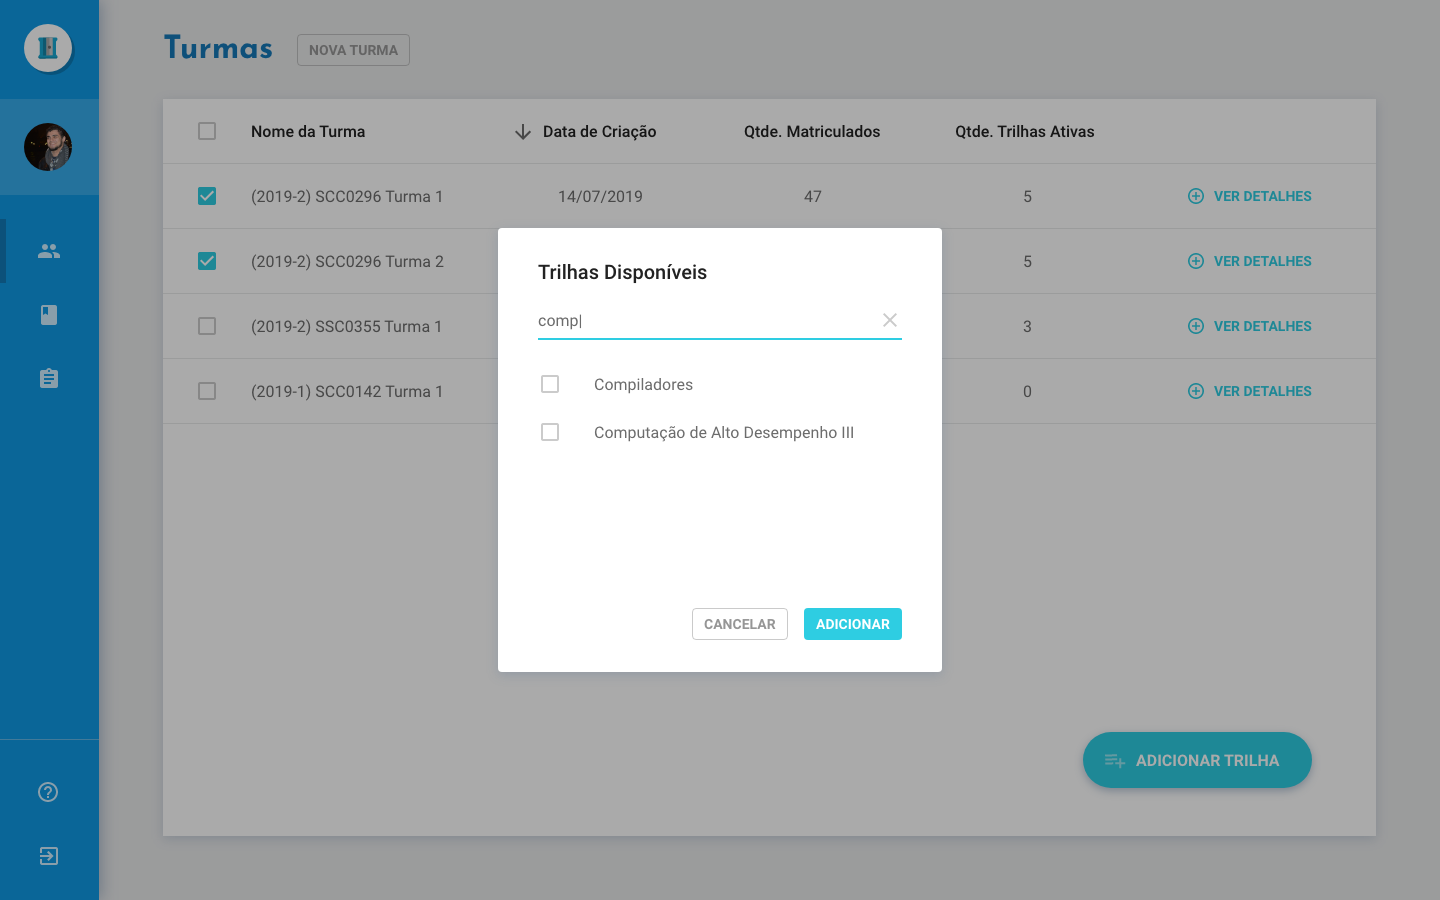
\includegraphics[width=\linewidth]{images/mocks/turmaAddTrackSearch.png}
    \caption{Página de turmas da prova de conceito do sistema \emph{Sharpener}, 
    que o professor inscreve suas turmas em trilhas, com um filtro  aplicado.}%
    \label{fig:enroll_track2}
  \end{figure}


% Preparar e carregar exercícios
\subsection{Preparando exercícios}
% \Sref já coloca Seção
Para a preparação de novos exercícios que farão parte do banco de exercícios, o professor precisa
ter baixado, instalado e configurado a \emph{CLI}, da mesma forma descrita na \Sref{ssec:aluno}. Há um comando para criar um novo exercício. Nesse caso, o Professor deve invocar o comando com a sintaxe descrita em \cref{codigo:new}. Este comando criará um diretório novo diretório com os arquivos 
que deverão ser preenchidos pelo professor antes de submeter o exercício para o banco 
de exercícios. Os arquivos a serem preenchidos são: um arquivo chamado ``README.md'', contendo as instruções 
do que se espera no exercício, um arquivo contento testes, outro arquivo que conterá código produzido pelo aluno 
e um arquivo que contém uma solução para o exercício, escrito pelo professor.

\begin{codigo}[caption = {Comando para criar novos exercícios na \emph{CLI}}, label={codigo:new},language=bash, breaklines=true]
prof@usp:~$ sharpener exercise new <language> <exercise_name>

\end{codigo}

Se o Professor desejar adicionar dicas para o exercício, este deve preencher o arquivo escondido,
``.meta.json''. A chave \emph{``hints''} deve conter um \emph{Array} de \emph{Strings}, em que 
cada uma delas é uma dica. O campo ``topics'' deste mesmo arquivo pode ser preenchido para relacionar 
este exercício a estes tópicos.

Para submeter o exercício criado o professor deve executar o comando descrito por \cref{codigo:post} na 
pasta que contém o exercício.

\begin{codigo}[caption = {Comando para submeter novos exercícios na \emph{CLI}}, label={codigo:post},language=bash, breaklines=true]
prof@usp:~$ sharpener exercise post
\end{codigo}

Caso deseje alterar um exercício, poderá baixá-lo através do comando \cref{codigo:download_prof} e 
ressubmetê-lo pelo \cref{codigo:post}. Apenas professores estão autorizados a utilizar o 
\cref{codigo:download_prof} e ressubmissões só podem ser feitas por exercícios de autoria daquele 
professor.
\begin{codigo}[caption = {Comando para baixar exercícios em modo edição na \emph{CLI}}, label={codigo:download_prof},language=bash, breaklines=true]
prof@usp:~$ sharpener exercise download <language> <exercise_name>

\end{codigo}



%% Enunciados
%% Casos de teste
%% Dicas
%% Grupo de Exercícios Equivalentes/Alternativos
%\subsubsection{Exercícios incrementais}
Como trilhas contêm Grupos de Exercícios Equivalentes, que serão resolvidos de forma sequencial pelo aluno, 
é possível propor exercícios incrementais. O efeito é atingido montando Grupos de Exercícios Equivalentes que contenham apenas um exercício. Assim, o aluno não pode pedir outro exercício equivalente e 
deve passar naquela trilha por todos os incrementos propostos.

% Acompanhar uma turma ou um aluno
\newpage

\section{A \emph{API} (\emph{Application Programming Interface})}
\subsection{Especificação}
Para suprir as necessidades da \emph{CLI} e do 
\emph{Frontend}, a \emph{API Web} fornece vários recursos diferentes. Alguns destes recursos não são protegidos, enquanto outros necessitam de identificação, que é provida pelo seu token pessoal. Os recursos disponíveis são
descritos a seguir, em que nomes entre o símbolo de maior e menor significam nomes variáveis 
da \emph{URI}.
\begin{description}
\item[\texttt{/api/classes}]  Rota protegida que, se o usuário for um professor, mostra todas as turmas que este criou. Caso o usuário seja aluno, mostra todas as classes em que faz parte. 
Aceita apenas o método \emph{GET}.
\item[\texttt{/api/classes/<name>}] Rota protegida que aceita apenas o método \emph{PUT}, emitido por 
um professor. Cria uma turma com o nome especificado. Turmas de um mesmo professor precisam 
ter nomes diferentes.
\item[\texttt{/api/classes/<name>/<track>}] Rota protegida que permite apenas o método \emph{PUT}, emitido por 
um professor. Associa uma turma, identificada pelo nome e criado por este mesmo professor, em uma determinada trilha.
\item[\texttt{/api/enrollments/<invite\_token>}] Rota protegida que aceita apenas o método \emph{POST}. Inscreve o Aluno em determinado turma, identificada por um código de convite.
\item[\texttt{/api/exercises}] Rota que aceita apenas o método \emph{GET}. Lista exercícios do banco 
de exercícios, por ordem ascendente por nível de dificuldade. A rota aceita paginação por meio 
de duas \emph{query strings}: ``\emph{page\_size}'' e ``\emph{page}''.
\item[\texttt{/api/exercises/<language>}] Rota que aceita apenas o método \emph{GET}. Lista exercícios do banco 
de exercícios, que sejam da linguagem especificada, por ordem ascendente por nível de dificuldade. A rota aceita paginação por meio 
de duas \emph{query strings}: ``\emph{page\_size}'' e ``\emph{page}''.
\item[\texttt{/api/exercises/<language>/<name>}] Rota protegida que aceita os método \emph{GET} e
\emph{PUT}. Ao receber um méotodo \emph{GET}, de um professor, mostra todos os detalhes relativos ao exercício, como a descrição do problema e \emph{URI}s para download dos artefatos associados. Se o ponto de acesso receber um \emph{PUT}, cria ou atualiza o exercício no banco de exercícios. Exercícios só podem ser atualizados se o criador do exercício foi o professor emissor da requisição.
\item[\texttt{/api/submissions/<submission\_token>}] Rota protegida que aceita  métodos \emph{POST} e \emph{GET}. O método \emph{GET} retorna todos os detalhes do exercício relativa a submissão referenciada 
por um \emph{token} de submissão e o método \emph{POST} registra uma tentativa de submissão.
\item[\texttt{/api/submissions/<submission\_token>/forfeit}] Rota protegida que aceita  métodos \emph{POST}.
Uma submissão nesta rota informa ao sistema que o estudante desiste da resolução deste exercício. A rota 
devolve a solução do exercício e uma \emph{token} de submissão de um novo exercício do mesmo Grupo de Exercícios Equivalentes. A desistência só será aceita se houver um novo exercício do Grupo de Exercícios Equivalentes, o qual o aluno ainda não tentou resolver.
\item[\texttt{/api/topics}] Rota que aceita apenas o método \emph{GET}. Mostra todos os tópicos já abordados por exercícios do banco de exercícios.
\item[\texttt{/api/topics/<language>}] Rota que aceita apenas o método \emph{GET}. Mostra todos os tópicos já abordados por exercícios do banco de exercícios, filtrados pela língua que foi 
provida na \emph{URI}.
\item[\texttt{/api/tracks/<track\_name>}] Rota protegida que aceita apenas o método \emph{PUT} de Professores. 
Cria uma nova trilha com o nome indicado na \emph{URI}, contanto que o professor não tenha criado outra com este mesmo nome.
\item[\texttt{/api/tracks/<track\_name>/classes/<class\_name>}] Rota protegida que aceita apenas o método \emph{PUT} de Professores. Matricula todos os alunos 
presentes na turma, que ainda não foram matriculados, na trilha que foi associada a uma turma específica. Ao invocar este ponto de acesso, o sistema cria 
, para cada aluno naquela turma e cada Grupo de Exercícios Equivalentes, uma submissão em estado pendente. Cada submissão é associada a um exercício aleatoriamente 
escolhido do Grupo de Exercícios Equivalentes. Se novos Alunos ingressarem na turma e uma nova requisição for disparada  ao ponto de acesso, submissões serão apenas 
criadas aos novos Alunos.
\item[\texttt{/api/healthcheck}] Rota que aceita apenas o método \emph{GET}. Informa se o serviço está funcionando corretamente e se a conexão com o banco de dados foi comprometida. Esta rota foi feita para que uma sonda externa faça esta consulta, e que caso haja alguma anormalidade, que um novo contêiner da aplicação seja iniciado e o tráfego direcionado a ele. 
\end{description}

Fora da \emph{API}, existem duas outras rotas, criadas especificamente para o \emph{Frontend}.
A primeira delas está exposta na raiz do servidor e serve o \emph{template} contendo o código da  \emph{single page application} do \emph{Frontend}. Uma outra rota, servida em ``\texttt{/authenticate}'', também se fez necessária para ser possível autenticação do usuário pelo \emph{Github}. A rota salva na sessão do usuário que está logado e suas informações, para que a maior parte dos acessos futuros não necessitem repetir os passos de autenticação federada.
% Pontos de acesso, etc. etc.

\subsection{Implementação} % DA API
A implementação do protótipo do servidor foi desenvolvida na linguagem \emph{Python} em conjunto 
com o \emph{microframework Web}, \emph{Flask}. Escolheu-se o banco de dados relacional \emph{PostgreSQL} para armazenamento dos dados e a \emph{ORM} \hyperref[link:sqlalchemy]{\emph{SQLAlchemy}}  para mapear 
o esquema do banco de dados em classes. 

Pela comodidade e confiabilidade, escolheu-se utilizar um serviço de computação em nuvem ao invés de rodar o projeto \emph{On-Premisses}. A \emph{Cloud} escolhida foi a \hyperref[link:gcp]{\emph{Google Cloud Plataform}}. 
Fez-se uso do serviço de armazenamento de intervalos para salvar arquivos de exercícios e submissões,
e do \hyperref[link:appengine]{\emph{AppEngine}}, o  \emph{Platform as a Service} da provedora, para hospedar a aplicação.
% Discutir o protótipo do servidor: repassar as opções de cloud, banco, etc

Detalhes de implementação estão detalhadas no \Aref{chapter:implementacao}. Os repositórios dos três projetos, \emph{API Web},  \emph{CLI} e \emph{Frontend} são de domínio público, e são de código aberto, aceitando assim contribuições de interessados.

\section{Resultados}
Um protótipo de sistema foi desenvolvido, conforme discutido anteriormente. Nesta versão alfa, testaram-se \emph{workflows} básicos 
como as sequências discutidas nas \Sref{ssec:aluno} e \Sref{ssec:professor}; em resumo foi testado a interação com turmas, trilhas e exercícios. Os \emph{endpoints} presentes na \emph{API} pareceram suficientes para as atividades  
propostas e a \emph{CLI} provou-se uma forma interessante do Aluno interagir com a plataforma. Nem todo o \emph{design} do \emph{frontend} foi, de fato, implementado. Como o foco do projeto foi, principalmente, o desenvolvimento da \emph{CLI} e da \emph{API Web},  apenas a parte vital para execução dos fluxos anteriores foi desenvolvida.

Para os testes na versão alfa foram extraídos exercícios de outra plataforma, \emph{exercism}. Através de um \emph{script}, de forma automática, inseriu-se diversos exercícios no banco de dados. 222 exercícios, de duas linguagens diferentes, compuseram o conjunto extraído, exercícios os quais tiveram 157 tópicos distintos associados a eles. Com esta variedade de exercícios, pôde-se ter uma ideia de como o sistema se comportaria em versões futuras.


\chapter{Conclusão}
\label{chapter:conclusao}
\section{Contribuições}
O presente trabalho pode ser entendido como um exercício de \emph{design} de software educativo para o ensino de programação, com destaque para as funcionalidades de apoio ao aluno, tais como: 
\begin{itemize}
    \item acesso a dicas por exercício, 
    \item acesso à resposta com possibilidade de resolver um exercício alternativo, e 
    \item exercícios formulados de forma incremental.
\end{itemize}
O acompanhamento de alunos com base nas formas de apoio acionadas por eles também é um diferencial.

Como prova de conceito, foi desenvolvido um protótipo funcional, para o qual foram parcialmente projetados e implementados: 
\begin{itemize}
    \item uma API Web de acesso, 
    \item um modelo conceitual para os dados, 
    \item interface de linha de comando e 
    \item interface web.
\end{itemize}
\section{Trabalhos futuros}
\begin{itemize}
    \item É importante buscar alguma forma de validação das ideias a partir da aplicação do sistema em disciplinas de programação.
    Em particular, deve-se observar como o aluno se apropria das formas diferenciadas de apoio, e qual o impacto disso na evolução do aluno ao longo da disciplina.
    \item A ideia de geração parcialmente aleatória de exercícios tem afinidade com a ideia de Grupo de Exercícios Equivalentes/Alternativos. A proposta é criar \emph{templates} de enunciados com pontos de inserção a serem preenchidos aleatoriamente. Os \emph{templates} se estenderiam também aos casos de teste, e às soluções armazenadas.
    \item O sistema deveria aceitar a importação de ontologias educacionais para objetivos pedagógicos, avaliação e outras formas de integração com sistemas educacionais.
\end{itemize}



% \chapter{Instalando o abnTeX2}
% \label{chapter:instalando-abntex}
% 
A instalação do \emph{abnTeX2} varia de acordo com o sistema operacional empregado pelo usuário. Aqui serão apresentadas as formas de instalação nos sistemas mais utilizados atualmente no curso de ciência da computação do Câmpus Catalão, a saber: Linux (Ubuntu 12.04), Mac OS X e Windows 7

\section{Linux (Ubuntu 12.04)}

Se você já instalou o Tex Live via apt-get, basta seguir os seguintes comandos:

\begin{enumerate}

\item Baixe os arquivos de instalação do abnTeX2 (\url{http://code.google.com/p/abntex2/downloads/list}). Nesse link você também encontra a documentação e exemplos de uso.
\item Extraia o conteúdo do arquivo baixado na pasta texmf local, geralmente /usr/local/share/texmf. 
\item Em um Terminal: extraia o ZIP: \emph{unzip abntex2.tds.zip} em qualquer local;
\item copie o conteúdo extraído para o destino: \emph{cp abntex2/* /usr/local/share/texmf};
\item Em um Terminal digite: \emph{sudo texhash}
\item Pronto!
\end{enumerate}

\section{Mac OS}

Primeiramente, deve-se abrir o terminal do Mac que pode ser encontrado em Aplicativos/Utilitários - buscando pelo Finder.  E seguir os comandos abaixo:
\begin{enumerate}
\item Baixe os arquivos de instalação do abnTeX2 (\url{http://code.google.com/p/abntex2/downloads/list}). Nesse link você também encontra a documentação e exemplos de uso.
\item Extraia o conteúdo do arquivo baixado na pasta \emph{texmf} local, geralmente \emph{/usr/local/texlive/texmf-local}
\item Em um Terminal digite: \emph{sudo texhash}
\item Pronto!
\end{enumerate}
 
 \section{Windows 7}

\subsection{Instalar/atualizar pelo Package Manager (recomendado)}

Geralmente o abnTeX2 é baixado e instalado automaticamente pelo MiKTeX quando o usuário compila pela primeira vez um dos modelos do abnTeX2. Porém, caso isso não ocorra, siga os passos seguintes:

\begin{enumerate}
\item Clique em Iniciar/Start -> Todos os Programas/All Programs -> MiKTeX -> Package Manager;
\item Clique em Repository / Synchronize;
\item Clique com o botão direito sobre \emph{abntex2} na lista e selecione Install (ou Update, caso já esteja instalado);
\item Pronto!
\end{enumerate}

\subsection{Instalar/atualizar manualmente}

Você apenas precisará utilizar a instalação manual no caso de:

\begin{enumerate}
\item o abnTeX2 não estar na lista de pacotes do MiKTeX por alguma razão;
\item você não poder utilizar uma conexão com a Internet no momento da instalação;
\item a versão do abnTeX2 no MiKTeX estar desatualizada em relação à versão disponível no CTAN.
\end{enumerate}
Em qualquer caso, lembre-se de remover uma eventual instalação anterior do abnTeX2 . Se houver instalado pelo Package Manager, remova o abnTeX2 também por ele.

Passos para instalação manual do abnTeX2 no MiKTeX:

\begin{enumerate}
\item Baixe os arquivos de instalação do abnTeX2 (abntex2.tds-vX.X.zip). Nesse link você também encontra a documentação e exemplos de uso.
\item Extraia o conteúdo do arquivo baixado em uma pasta qualquer;
\item Você pode criar uma pasta abntex2, por exemplo, em $C:\backslash abntex2\backslash$;
\item Consulte http://www.tex.ac.uk/cgi-bin/texfaq2html?label=install-where para outras informações;
\item Clique em Iniciar/Start -> Todos os Programas/All Programs -> MiKTeX -> Settings;
\item Na aba Roots, adicione o diretório recém criado;
\item Na aba General, clique em Refresh FNDB, OU, se preferir, em um Terminal digite initexmf --update-fndb;
\item Pronto!
\end{enumerate}

% \chapter{Orientações Gerais}
% \label{chapter:orientacoes-gerais}
% 

\section{Codificação dos arquivos: UTF8}

A codificação de todos os arquivos do \abnTeX\ é \texttt{UTF8}. É necessário que
você utilize a mesma codificação nos documentos que escrever, inclusive nos
arquivos de base bibliográficas |.bib|.



\section{Inclusão de outros arquivos}\label{sec-include}

É uma boa prática dividir o seu documento em diversos arquivos, e não
apenas escrever tudo em um único. Esse recurso foi utilizado neste
documento. Para incluir diferentes arquivos em um arquivo principal,
de modo que cada arquivo incluído fique em uma página diferente, utilize o
comando:

\begin{verbatim}
   \include{documento-a-ser-incluido}      % sem a extensão .tex
\end{verbatim}

Para incluir documentos sem quebra de páginas, utilize:

\begin{verbatim}
   \input{documento-a-ser-incluido}      % sem a extensão .tex
\end{verbatim}



%\section{Remissões internas}

%Ao nomear a \autoref{tab-nivinv} e a \autoref{fig_circulo}, apresentamos um exemplo de remissão interna, que também pode ser feita quando indicamos o \autoref{cap_exemplos}, que tem o nome \emph{\nameref{cap_exemplos}}. O número do capítulo indicado é \ref{cap_exemplos}, que se inicia à \autopageref{cap_exemplos}\footnote{O número da página de uma remissão pode ser obtida também assim: \pageref{cap_exemplos}.}.
%Veja a \autoref{sec-divisoes} para outros exemplos de remissões internas entre seções, subseções e subsubseções.

%O código usado para produzir o texto desta seção é:

%\begin{verbatim}
%Ao nomear a \autoref{tab-nivinv} e a \autoref{fig_circulo}, apresentamos um
%exemplo de remissão interna, que também pode ser feita quando indicamos o
%\autoref{cap_exemplos}, que tem o nome \emph{\nameref{cap_exemplos}}. 
%O número
%do capítulo indicado é \ref{cap_exemplos}, que se inicia à
%\autopageref{cap_exemplos}\footnote{O número da página de uma remissão pode ser
%obtida também assim:
%\pageref{cap_exemplos}.}.
%Veja a \autoref{sec-divisoes} para outros exemplos de remissões internas entre
%seções, subseções e subsubseções.
%\end{verbatim}



\section{Consulte o manual da classe \textsf{abntex2}}

Consulte o manual da classe \textsf{abntex2} \cite{abntex2classe} para uma
referência completa das macros e ambientes disponíveis. 

Além disso, o manual possui informações adicionais sobre as normas ABNT
observadas pelo \abnTeX\ e considerações sobre eventuais requisitos específicos
não atendidos, como o caso da \citeonline[seção 5.2.2]{NBR14724:2011}, que
especifica o espaçamento entre os capítulos e o início do texto, regra
propositalmente não atendida pelo presente modelo.



\section{Precisa de ajuda?}

Consulte a FAQ com perguntas frequentes e comuns no portal do \abnTeX:
\url{https://code.google.com/p/abntex2/wiki/FAQ}.

Inscreva-se no grupo de usuários \LaTeX:
\url{http://groups.google.com/group/latex-br}, tire suas dúvidas e ajude
outros usuários.

Participe também do grupo de desenvolvedores do \abnTeX:
\url{http://groups.google.com/group/abntex2} e faça sua contribuição à
ferramenta.



\section{Você pode ajudar?}

Sua contribuição é muito importante! Você pode ajudar na divulgação, no
desenvolvimento e de várias outras formas. Veja como contribuir com o \abnTeX\
em \url{https://code.google.com/p/abntex2/wiki/ComoContribuir}.

% \chapter{Configuração dos Elementos Pré-Textuais}
% \label{chapter:config-pre-textual}
% A configuração de diversas opções e principalmente dos elementos pré-textuais é realizada com comandos específicos inseridos antes do comando \comando{begin\{document\}}. As informações do documento são configuradas através dos comandos:

\begin{description}

 \item[\comando{titulo\{T\}}] Título do trabalho (substitua T pelo título do trabalho);

 \item[\comando{autor[REF]\{N\}}] Nome do autor do trabalho (onde REF é como o nome do autor é referenciado e N é o nome do autor);

 \item[\comando{orientador\{T\}\{O\}}] Nome do professor orientador do trabalho. Caso seja uma orientadora pode ser usado o comando \comando{orientador[Orientadora:]\{T\}\{O\}} (sendo que T é a titulação do professor e O é o nome do orientador);

 \item[\comando{coorientador\{T\}\{C\}}] Nome do professor coorientador do trabalho. Caso seja uma coorientadora pode ser usado um comando análogo a definição de orientadora  empregando o comando \comando{coorientador[Coorientadora:]\{T\}\{C\}}(sendo que T é a titulação do professor e C é o nome do orientador);

 
 \item[\comando{curso\{EP\}\{NP\}}] Dados do programa de Pós-Graduação (onde EP é a especialidade que será atribuída ao pós-graduando e NP é o nome do programa de pós-graduação.  Exemplo: \comando{curso\{Ciências -- Ciências de Computação e Matemática Computacional\}\{Ciências de Computação e Matemática Computacional\}};
 
 \item[\comando{data\{dia\}\{mês\}\{ano\}}] Configuração da data do depósito do documento;

 \item[\comando{textoresumo\{TR\}\{PC\}}] Texto do resumo (TR) e palavras-chave (PC) do documento sendo separadas por vírgula. Se o idioma do resumo for diferente do declarado no documento, pode ser usado o comando \comando{textoresumo[L]\{TR\}\{PC\}} (sendo que L é a linguagem do resumo).
 
\end{description}

As opções seguintes correspondem também as configurações dos elementos pré-textuais, porém seu uso é opcional: 

\begin{description}

 \item[\comando{textodedicatoria\{TD\}}] Texto referente a dedicatória do trabalho (TD). Caso o texto esteja em um arquivo separado (recomendado para que o projeto fique modularizado e os documentos mais limpo), deve utilizar o comando \comando{textodedicatoria*\{ARQ\}}, em que ARQ é o nome do arquivo, incluindo o caminho do diretório se necessário;

 \item[\comando{textoagradecimentos\{TA\}}] Texto referente aos agradecimentos do trabalho (TA). Caso o texto esteja em um arquivo separado (recomendado para que o projeto fique modularizado e os documentos mais limpo), deve utilizar o comando \comando{textoagradecimentos*\{ARQ\}}, em que ARQ é o nome do arquivo, incluindo o caminho do diretório se necessário;

 \item[\comando{incluilistadefiguras}] Comando para inclusão da lista de figuras. Deve-se utilizar este comando somente quando o ambiente \textbf{figure} for utilizado no documento;
 
 \item[\comando{incluilistadetabelas}] Comando para inclusão da lista de tabelas. Deve-se utilizar este comando somente quando o ambiente \textbf{table} for utilizado no documento;
  
 \item[\comando{incluilistadequadros}] Comando para inclusão da lista de quadros. Deve-se utilizar este comando somente quando o ambiente \textbf{quadro} for utilizado no documento;
   
 \item[\comando{incluilistadealgoritmos}] Comando para inclusão da lista de algoritmos. Deve-se utilizar este comando somente quando o ambiente \textbf{algoritmo} for utilizado no documento;
    
 \item[\comando{incluilistadecodigos}] Comando para inclusão da lista de figuras. Deve-se utilizar este comando somente quando o ambiente \textbf{codigo} for utilizado no documento;
 
 \item[\comando{incluilistadesiglas}] Comando para inclusão da lista de siglas e abreviaturas. Deve-se utilizar este comando somente quando existirem siglas e abreviaturas no documento, com a utilização do comando \comando{sigla\{S\}\{DS\}} ou \comando{sigla*\{S\}\{DS\}};

 \item[\comando{incluilistadesimbolos}] Comando para inclusão da lista de símbolos. Deve-se utilizar este comando somente quando existirem símbolos no documento, com a utilização do comando \comando{simbolo\{S\}\{DS\}}.
 
\end{description}

% \chapter{Corpos Flutuantes}
% \label{chapter:corpos-flutuantes}
% 
Corpos flutuantes são elementos não textuais, como figuras e tabelas, que complementam as informações do texto. Neste capítulo são expostos breves exemplos dos corpos flutuantes disponíveis na classe \textit{icmc}.

Na \autoref{secao:figuras} é mostrado como inserir figuras, a \autoref{secao:tabelas_e_quadros} explica como incluir tabelas e quadros, a \autoref{secao:algoritmos_e_codigos} demostra como trabalhar com algoritmos e códigos-fonte e a \autoref{secao:outros-ambientes} explica como definir outros ambientes para serem utilizados, como para gráficos e diagramas.

\section{Figuras}
\label{secao:figuras}

A inserção de figuras é realizada normalmente através do comando \comando{begin\{figure\}}. Na \autoref{figura:logomarca_usp} é exibida a logomarca da USP com o pacote \textit{graphicx}. Já a \autoref{figura:exemplo_grafo} mostra um exemplo de grafo com o pacote \textit{xy}. De acordo com as normas ABNT a lista de figuras é um elemento opcional do documento, para incluí-la é preciso inserir o comando \comando{incluidelistafiguras} antes do início do documento.

Observe que, segundo a \citeonline[seções 4.2.1.10 e 5.8]{NBR14724:2011}, as
ilustrações devem sempre ter numeração contínua e única em todo o documento. Além disso, deve ser incorporado ao corpo flutuante do tipo figura, além da legenda, a fonte de onde esta foi extraída. Se a figura foi confeccionada pelo próprio autor, deve se colocar "Elaborada pelo autor".

\begin{citacao}
Qualquer que seja o tipo de ilustração, sua identificação aparece na parte
superior, precedida da palavra designativa (desenho, esquema, fluxograma,
fotografia, gráfico, mapa, organograma, planta, quadro, retrato, figura,
imagem, entre outros), seguida de seu número de ordem de ocorrência no texto,
em algarismos arábicos, travessão e do respectivo título. Após a ilustração, na
parte inferior, indicar a fonte consultada (elemento obrigatório, mesmo que
seja produção do próprio autor), legenda, notas e outras informações
necessárias à sua compreensão (se houver). A ilustração deve ser citada no
texto e inserida o mais próximo possível do trecho a que se
refere. \cite[seções 5.8]{NBR14724:2011}
\end{citacao}

\begin{figure}[htb]
 \caption{Logomarca da USP}
 \label{figura:logomarca_usp}
 \centering
 
\includegraphics[scale=0.3]{images/usp-logo}
 \fdireta{usp:logo}
\end{figure}


\begin{figure}[htb]
\caption{Exemplo de grafo}
\label{figura:exemplo_grafo}
\centering
\begin{scriptsize}
$$
\xymatrix@R20pt@C10pt{
 & & & & vr \ar[dlll] \ar[dl] \ar[d] \ar[dr] \ar[drr] \ar[drrr] & & & \\
 & (a_3, b_2, c_1) \ar[d]^{\varphi_2} \ar[dl]_{\varphi_1} & & (a_3, b_2, c_2) \ar[d]^{\varphi_2} \ar[dl]_{\varphi_1} & (a_1, b_1, c_1) & (a_1, b_1, c_2) & (a_1, b_2, c_1) & (a_1, b_2, c_2) \\
 (a_2, b_2, c_1) \ar[dr]_{\varphi_3} & (a_3, b_1, c_1) \ar[d]^{\varphi_1} & (a_2, b_2, c_2) \ar[dr]_{\varphi_3} & (a_3, b_1, c_2) \ar[d]^{\varphi_1} & & & & \\
& (a_2, b_1, c_1)  & & (a_2, b_1, c_2) & & & & \\
}
$$
\end{scriptsize}
\fautor
\end{figure}

A classe \textit{icmc} traz algum comando que auxiliam na inserção da legenda, para utilizá-los basta substituir o \comando{fonte\{\}} por um dos seguintes comando conforme necessário:

\begin{description}

 \item[\comando{fautor}] Insere o texto \aspas{Elaborada pelo autor} como fonte da figura;

 \item[\comando{fadaptada[INF]\{REF\}}] Insere um texto informando que a figura foi adaptada de alguma referência bibliográfica (REF). INF refere-se ao local específico de onde a imagem foi extraída, como por exemplo o número da página. Além disso, INF é um parâmetro opcional e pode receber qualquer cadeia de texto;

 \item[\comando{fdireta[INF]\{REF\}}] Insere um texto informando que a figura próvem diretamente de alguma referência bibliográfica (REF). INF refere-se ao local específico de onde a imagem foi extraída, como por exemplo o número da página. Além disso, INF é um parâmetro opcional e pode receber qualquer cadeia de texto;
 
 \item[\comando{fdadospesquisa}] Insere o texto \aspas{Dados da pesquisa.} como fonte da figura;
 
\end{description}



\section{Tabelas e Quadros}
\label{secao:tabelas_e_quadros}

A inserção de tabelas e quadros é feita de forma semelhante a inserção de figuras, porém são utilizados os ambientes \textit{table} e \textit{quadro}. A principal diferença entre tabelas e quadros, de acordo com \citeonline{silveira:2006:manual_tcc}, é que as tabelas são destinadas para informações numéricas e os quadros são mais adequados para informações textuais. Em geral, as tabelas devem estar padronizadas conforme o padrão do
\citeonline{ibge1993} requerido pelas normas da ABNT para documentos técnicos e
acadêmicos.

Como exemplos foram inseridas a \autoref{tabela:lista_produtos} que exibe uma de lista de produtos (construída em \LaTeX) e a Tabela \autoref{tabela:populacao_america_sul} que mostra a população dos países da América do Sul (construída segundo o padrão do IBGE). Foi inserido também o \autoref{quadro:editores_texto_livres} com alguns editores que podem ser usados para se trabalhar com \LaTeX para demonstrar a inserção de quadros.

 A lista de tabelas também é um elemento opcional que pode ser incluída com o comando \comando{incluidelistatabelas} antes do início do documento. O mesmo acontece com a lista de quadros que pode ser incluída com o comando \comando{incluidelistaquadros}.

\begin{table}[htb]
\centering
\caption{Lista de produtos}
\label{tabela:lista_produtos}
\begin{tabularx}{\textwidth}{X|l|r|r|r} \hline
Produto      & Unidade & Preço (R\$) & Quantidade & Total (R\$) \\ \hline
Arroz        & Kg      & 2,00        & 550        & 1.100,00    \\
Óleo de Soja & L       & 2,50        & 500        & 750,00      \\
Açucar       & Kg      & 3,00        & 100        & 300,00      \\ \hline
\end{tabularx}
\fdadospesquisa
\end{table}

\begin{table}[htb]
\IBGEtab{%
  \caption{População dos países da América do Sul} \label{tabela:populacao_america_sul}
}{%
\begin{tabular}{r|p{3cm}|r}        
\toprule
Código  & País            & População   \\ \midrule \midrule
1       & Brasil          & ~~~~~~191.480.630 \\ \midrule 
2       & Argentina       &  39.934.100 \\ \midrule 
3       & Colômbia        &  46.741.100 \\ \midrule 
4       & Paraguai        &   9.694.200 \\ \midrule 
5       & Uruguai         &   3.350.500 \\ \midrule 
6       & Peru            &  28.221.500 \\ \midrule 
7       & Equador         &  13.481.200 \\ \midrule 
8       & Bolívia         &   9.694.200 \\ \midrule 
9       & Venezuela       &  28.121.700 \\ \midrule 
10      & Chile           &  16.803.000 \\ \bottomrule
\end{tabular}
}{%
  \fdireta{wikipedia:2011:america_sul}%
  \nota{Esta é uma nota, que diz que os dados são baseados na
  regressão linear.}%
  \nota[Anotações]{Uma anotação adicional, que pode ser seguida de várias
  outras, porém são opcionais.}%
  }
\end{table}

\begin{quadro}[htb]
\caption{Editores de Texto Livres}
\label{quadro:editores_texto_livres}
\centering
\begin{tabular}{|l|l|r|}        \hline
Editor     & Multiplataforma & Específico para Latex \\ \hline
Kwriter    & Sim             & Não                   \\
Texmaker   & Sim             & Sim                   \\
Kile       & Sim             & Sim                   \\
Geany      & Sim             & Não                   \\ \hline
\end{tabular}
\end{quadro}

\section{Algoritmos e Códigos}
\label{secao:algoritmos_e_codigos}

Além dos corpos flutuantes convencionais para inserir figuras (\comando{begin\{figure\}}) e tabelas (\comando{begin\{table\}}), a classe \textit{icmc} possui mais dois tipos de corpos flutuantes um para algoritmos (\comando{begin\{algoritmo\}}) e outro para códigos-fonte (\comando{begin\{codigo\}}). A utilização de um ou de outro fica a critério do usuário. Como exemplo temos o \autoref{algoritmo:mdc1} que calcula o máximo divisor comum entre dois números e os Códigos-fonte \ref{codigo:notas_alunos} e \ref{codigo:metodo_leitura} que são uma consulta na \sigla{SQL}{\textit{Structured Query Language}} e uma sobrotina em \textit{Java}.

%\begin{algoritmo}[htb]
\begin{algoritmo}
%\begin{algorithmic}[1]
\caption{Algoritmo para cálculo de máximo divisor comum MDC($n_1$,$n_2$)}
\label{algoritmo:mdc1}

 \KwIn{Dois números inteiros ($n_1, n_2$)}
 \If(\tcp*[f]{Garante que o maior número seja $n_1$}){$n_2 > n_1$}
   {troca valores de $n_1$ e $n_2$}
 \Repeat{$r > 0$}{
    $r \leftarrow$ resto da divisão de $n_1$ por $n_2$
    $n_1 \leftarrow n_2$
    $n_2 \leftarrow r$
 }
 \Return $n_1$
%\end{algorithmic}
\end{algoritmo}
%\end{algoritmo}

%\begin{codigo}[htb]
%\caption{Consulta SQL}
%\label{codigo:notas_alunos}
%\hrule
\begin{codigo}[caption = {Consulta SQL}, label={codigo:notas_alunos},language=SQL, breaklines=true]
SELECT a.nome_aluno AS aluno,
       d.nome_disciplina AS disciplina,
       m.nota AS nota
FROM aluno AS a,
     disciplina AS d,
     matriculado AS m
WHERE a.id_aluno = m.id_aluno
  AND d.id_disciplina = m.id_disciplina
ORDER BY a.nome_aluno, d.nome_disciplina;
\end{codigo}
%\end{codigo}

%\begin{codigo}[htb]
%\caption{Subrotina para obter uma entrada do usuário}
%\label{codigo:metodo_leitura}
%\hrule
\begin{codigo}[caption={Subrotina para obter uma entrada do usuário}, label={codigo:metodo_leitura}, language=Java, breaklines=true]
public static String Leitura(){
    BufferedReader reader = new BufferedReader(new InputStreamReader(System.in));
    try {
        return reader.readLine(); // Lê uma linha pelo teclado
    } catch (IOException e) {
        e.printStackTrace();
        return "";
    }
}
\end{codigo}
%\end{codigo}

Existem diversos outros pacotes disponíveis para escrever algoritmos e códigos. Nos exemplos anteriormente foram utilizados o pacote \textit{algorithm} para definição do ambiente algoritmo e \textit{listings} para a definição do ambiente de código-fonte. O pacote \textit{algorithm} é usado para escrever algoritmos em alto nível \cite{janos:2005:algpseudocode}. Já o pacote \textit{listings} serve para escrever os códigos em diversas linguagens de programação \cite{moses:2006:listings}.

Caso sejam utilizados os ambientes de algoritmos e código podem ser incluídos os comandos \comando{incluidelistaalgoritmos} e \comando{incluidelistacodigos} antes do \comando{begin\{document\}} para que a lista de algoritmos e a lista de código sejam criadas.


\section{Ambientes Matemáticos}

A classe \textit{icmc} provê os seguintes ambientes matemáticos:
\begin{itemize}
 \item Teoremas (\comando{begin\{teorema\}[\ ]} ... \comando{begin\{teorema\}});
 \item Proposição (\comando{begin\{proposicao\}[\ ]} ... \comando{begin\{proposicao\}});
 \item Lema (\comando{begin\{lema\}[\ ]} ... \comando{begin\{lema\}});
 \item Corolário (\comando{begin\{corolario\}[\ ]} ... \comando{begin\{corolario\}});
 \item Exemplo (\comando{begin\{exemplo\}[\ ]} ... \comando{begin\{exemplo\}});
 \item Observação (\comando{begin\{observacao\}[\ ]} ... \comando{begin\{observacao\}});
 \item Definição (\comando{begin\{definicao\}[\ ]} ... \comando{begin\{definicao\}});
 \item demonstracao (\comando{begin\{demonstracao\}[\ ]} ... \comando{begin\{demonstracao\}}).
\end{itemize}

Abaixo temos um exemplo de proposição com sua demonstração:
\begin{proposicao}
 Sejam $a$ e $b$ reais, tais que $0<a<b$. Então $a^2<b^2$.
\end{proposicao}
\begin{demonstracao}
 Pela hipótese concluímos que $(b+a)>0$ e $(b-a)>0$.

Como $b^2-a^2=(b+a)(b-a)$ concluímos que $b^2-a^2>0$, ou seja, $a^2<b^2$.
\end{demonstracao}

Neste documento tratamos brevemente apenas dos ambientes mencionados anteriormente. Contudo, para escrever expressões matemáticas complexas é preciso estudar uma documentação mais específica como em \citeonline{cassagojr:1997:amslatex}.

Alguns dos ambientes matemáticos da classe \textit{icmc} podem ser usados também para outras finalidades como exemplos e definições.


\section{Definição de outros ambientes}
\label{secao:outros-ambientes}

O classe \textit{icmc} permite a criação de outros ambientes, além dos citados nas seções anteriores, caso seja necessário. Isso é possível graças a extensão da classe \textit{abntex}. O \autoref{codigo:novo-ambiente} deve ser inserido antes do início do documento para criação de um ambiente para gráficos. Para definição de outros ambientes, basta seguir o modelo.


\begin{codigo}[caption={Definição do ambiente \textbf{grafico}}, label={codigo:novo-ambiente}, language=Tex, breaklines=true]
\makeatletter

% Novo list of (listings) para GRÁFICOS --------------------------
\newcommand{\graficoname}{Gráfico}
\newcommand{\graficorefname}{Gráfico}
\newcommand{\listofgraficosname}{Lista de gráficos}

\addto\captionsenglish{% ingles
    %% adjusts names from abnTeX2
    \newcommand{\graficoname}{Graph}
    \newcommand{\graficorefname}{Graph}
    \newcommand{\listofgraficosname}{List of graphs}
}

\newfloat[chapter]{grafico}{logr}{\graficoname}
\newlistof{listofgraficos}{logr}{\listgraficoname}
\newlistentry{grafico}{logr}{0}

% configurações para atender às regras da ABNT
\renewcommand{\thegrafico}{\thechapter.\@arabic\c@grafico}
\setfloatadjustment{grafico}{\centering}
\renewcommand{\cftgraficoname}{\graficoname\space}
\renewcommand*{\cftgraficoaftersnum}{\hfill\textendash\hfill}
% ----------------------------------------------------------------

\makeatother
\end{codigo}

A utilização do novo ambiente no texto segue conforme o \autoref{codigo:usar-novo-ambiente}.

\begin{codigo}[caption={Como usar o ambiente \textbf{grafico}}, label={codigo:usar-novo-ambiente}, language=Tex, breaklines=true]
\begin{grafico}[htb]
\caption{Caption do gráfico}
\label{gra:modelo}
Este é o conteúdo do gráfico.
\end{grafico}
\end{codigo}

Comandos como \comando{autoref\{gra:modelo\}} funcionam normalmente.

Para imprimir a "Lista de gráficos" no documento, insira o \autoref{codigo:lista-novo-ambiente} na classe \textit{icmc}, de modo que ele seja impresso após a "Lista de ilustrações". O código deve ser inserido após a linha 1244.


\begin{codigo}[caption={Código para inserir lista de gráficos}, label={codigo:lista-novo-ambiente}, language=Tex, breaklines=true]
% ---
% inserir lista de gráficos
% ---
\pdfbookmark[0]{\listofgraficosname}{logr}
\listofgraficos*
\cleardoublepage
% ---
\end{codigo}

% \chapter{Listas}
% \label{chapter:listas}
% \section{Abreviaturas e Siglas}

A classe \textit{icmc} implementa a criação da lista de abreviaturas e siglas com o pacote \textit{nomencl}. A inserção de abreviaturas e siglas na lista é realizada com o comando \comando{sigla\{A\}\{B\}}, onde \textit{A} é a sigla e \textit{B} é o nome por extenso. Para se gerar a lista de siglas na parte pre-textual é preciso incluir o comando \comando{incluidelistasiglas} antes do início do documento. Além disto, a compilação do documento deve conter o comando \textit{makeindex} após duas compilações com o \textit{pdflatex}. Por exemplo, supondo que o documento principal tenha o nome de \textit{monografia}, podemos usar a seguinte sequência de comandos:
\begin{verbatim}
pdflatex monografia.tex
pdflatex monografia.tex
makeindex monografia.nlo -s nomencl.ist -o monografia.nls
pdflatex monografia.tex
\end{verbatim}

No Capítulo \ref{chapter:ferramentas-uteis} serão apresentadas algumas ferramentas que podem facilitar o processo de compilação do documento.

\section{Símbolos}

A definição de símbolos é semelhante a definição de siglas, porém deve ser usado o comando \comando{simbolo\{S\}\{DS\}}, onde \textit{S} é o símbolo e \textit{DS} é a descrição do símbolo. Como exemplo definimos os símbolos \simbolo{\mathbb{X}}{Variável X}$\mathbb{X}$ e \simbolo{\mathsf{I\!R}}{Conjunto dos números reais}$\mathsf{I\!R}$. Para incluir a lista de símbolos, basta usar o comando \comando{incluidelistasimbolos} antes do início do documento.


% \chapter{Ferramentas Úteis}
% \label{chapter:ferramentas-uteis}
% Existem diversas ferramentas para se trabalhar com \LaTeX. Duas ferramentas que merecem destaque são o editor \textit{Texmaker} exibido na Figura \ref{figura:texmaker} e o gerenciador de referências \textit{JabRef} mostrado na Figura \ref{figura:jabref}. Ambas ferramentas são livres e multiplataforma.

\begin{figure}[htb]
\caption{Tela do Texmaker}
 \label{figura:texmaker}
 \centering
 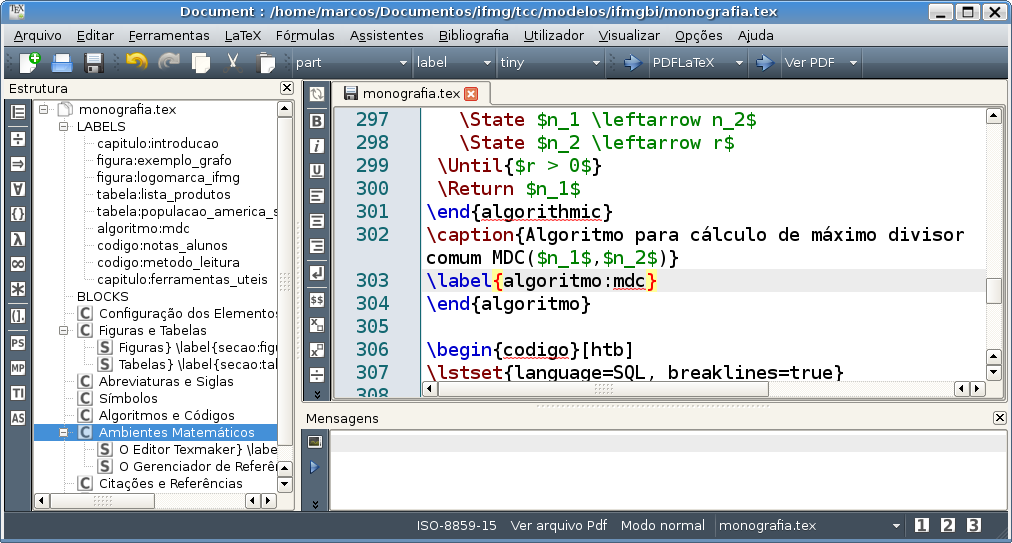
\includegraphics[width=\textwidth]{texmaker}
 \legend{Fonte: o autor.}
\end{figure}

\begin{figure}[htb]
 \caption{Tela do JabRef}
 \label{figura:jabref}
 \centering
 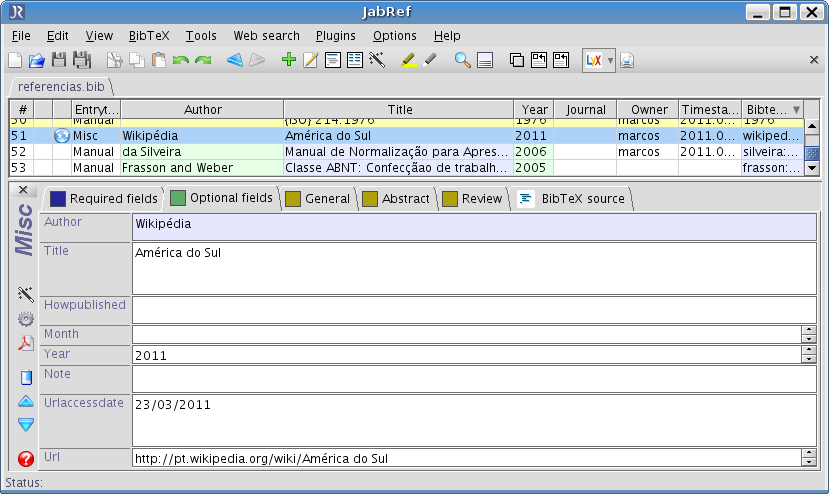
\includegraphics[width=\textwidth]{jabref}
\legend{Fonte: o autor.}
\end{figure}

O Texmaker pode ser obitido em \url{www.xm1math.net/texmaker} e o JabRef pode ser obtido em \url{jabref.sourceforge.ne}. É importante ressaltar que o Texmaker é apenas um editor, para compilar os documentos é necessário um ambiente \LaTeX instalado. Os ambientes Latex mais populares são o Texlive (\url{www.tug.org/texlive}) e o MiKTex (\url{miktex.org}).

% \chapter{Citações e Referências}
% \label{chapter:citacoes}
% Em documentos acadêmicos podem existir citações diretas e citações indiretas. As citações indiretas são feitas quando se reescreve uma referência consultada. Nas citações indiretas há duas formatações possíveis dependendo de como ocorre a citação no texto. Quando o autor é mencionado explicitamente  deve ser usado o comando \comando{citeonline\{\}}, nas demais situações é usado o comando \comando{cite\{\}}. No quadro \ref{figura:citacao_indireta_explicita} encontrasse um  exemplo de uso do comando \comando{citeonline\{\}}.

\begin{quadro}[htb]
\caption{Exemplo de citação indireta explícita} \label{figura:citacao_indireta_explicita}
\hrulefill

\lstset{language=Tex, breaklines=true}
\begin{lstlisting}
Segundo \citeonline{silveira:2006}, o trabalho de conclusão de curso deve seguir as normas da ABNT.
\end{lstlisting}

\hrulefill

Segundo \citeonline{silveira:2006:manual_tcc}, o trabalho de conclusão de curso deve seguir as normas da ABNT.

\hrulefill

%\legend{Fonte: o autor.}
\end{quadro}

Para especificar a página consultada na referência é preciso acrescentá-la entre colchetes com os comandos \comando{cite[página]\{\}} ou \comando{citeonline[página]\{\}}. No quadro \ref{figura:citacao_indireta_pagina} é mostrado um exemplo de citação com página específica.

\begin{quadro}[htb]
\caption{Exemplo de citação indireta não explícita} \label{figura:citacao_indireta_pagina}
\hrulefill

\lstset{language=Tex, breaklines=true}
\begin{lstlisting}
A folha de aprovação é um elemento obrigatório na monografia de projeto final de curso trabalho de conclusão de curso.  \cite[p.~10]{silveira:2006}.
\end{lstlisting}

\hrulefill

A folha de aprovação é um elemento obrigatório no trabalho de conclusão de curso.  \cite[p.~10]{silveira:2006:manual_tcc}.

\hrulefill

\end{quadro}

As citações diretas acontecem quando o texto de uma referência é transcrito literalmente. As citações diretas são curtas (até três linhas) são inseridas no texto entre aspas duplas. Conforme exemplo no quadro \ref{figura:citacao_direta_curta}.

\begin{quadro}[htb]
\caption{Exemplo de citação direta curta}
\label{figura:citacao_direta_curta}
\hrulefill

\lstset{language=Tex, breaklines=true}
\begin{lstlisting}
``Os quadros, ao contrário das tabelas, apresentam dados textuais e devem localizar-se o mais próximo do texto a que se referem'' \cite[p.~25]{silveira:2006}.
\end{lstlisting}

\hrulefill

``Os quadros, ao contrário das tabelas, apresentam dados textuais e devem localizar-se o mais próximo do texto a que se referem'' \cite[p.~25]{silveira:2006:manual_tcc}.

\hrulefill
\end{quadro}

As citações longas (com mais de 3 linhas) podem ser inseridas via \comando{begin\{citacao\}} conforme quadro \ref{figura:citacao_direta_longa}.

\begin{quadro}[htb]
\caption{Exemplo de citação direta longa}
\label{figura:citacao_direta_longa}
\hrulefill

\lstset{language=Tex, breaklines=true}
\begin{lstlisting}
\begin{citacao}
Síntese final do trabalho, a conclusão constitui-se de uma resposta à hipótese enunciada na introdução. O autor manifestará seu ponto de vista sobre os resultados obtidos e sobre o alcance dos mesmos. Não se permite a inclusão de dados novos nesse capítulo nem citações ou interpretações de outros autores \cite[p.~25]{silveira:2006}.
\end{citacao}
\end{lstlisting}

\hrulefill

\begin{citacao}
Síntese final do trabalho, a conclusão constitui-se de uma resposta à hipótese enunciada na introdução. O autor manifestará seu ponto de vista sobre os resultados obtidos e sobre o alcance dos mesmos. Não se permite a inclusão de dados novos nesse capítulo nem citações ou interpretações de outros autores \cite[p.~25]{silveira:2006:manual_tcc}.
\end{citacao}

\hrulefill

\end{quadro}


% ---
% Finaliza a parte no bookmark do PDF, para que se inicie o bookmark na raiz
% ---
% \bookmarksetup{startatroot}% 
% ---

% ----------------------------------------------------------
% ELEMENTOS PÓS-TEXTUAIS
% ----------------------------------------------------------
% \postextual

% ----------------------------------------------------------
% Referências bibliográficas
% ----------------------------------------------------------
\bibliography{references}

% ---------------------------------------------------------------------
% GLOSSÁRIO
% ---------------------------------------------------------------------

% Arquivo que contém as definições que vão aparecer no glossário
% \newword{1}{Agentes de usuário}{qualquer \textit{software} que recupera, processa e facilita a interação do usuário final com o conteúdo  Web. Como exemplo desses agentes, podem ser citados navegadores, reprodutores multimídia e tecnologias assistivas} 

\newword{2}{ATAG}{\textit{Authoring Tool Accessibility Guidelines} ou Diretrizes de acessibilidade para ferramentas de autoria. É um conjunto de diretrizes para desenvolvedores de qualquer ferramenta de criação para Web, como: simples editores HTML, ferramentas para exportar conteúdo para Web, ferramentas multimídia e sistemas de gerenciamento de conteúdo}

\newword{3}{DOM}{\textit{Document Object Model} ou Modelo de Objetos de Documentos. É uma especificação do W3C para organizar objetos de um documento em que se pode, dinamicamente, alterar e editar sua estrutura, conteúdo e estilo}

\newword{4}{Javascript}{é uma linguagem de \textit{script} para desenvolvimento de certos tratamentos 
que ocorrem lado do cliente, geralmente o navegador Web. Ela é utilizada geralmente quando 
é inconveniente ou impossível para o servidor para fazer esse tratamento}

\newword{5}{Stakeholder}{qualquer pessoa ou grupo, que legitima as ações de uma organização. É formado pelos funcionários da empresa, gestores, gerentes, proprietários, fornecedores, clientes, o Estado, credores, sindicatos e diversas outras pessoas ou empresas que estejam relacionadas com uma determinada ação ou projeto.}

\newword{6}{Tag}{ou etiqueta, é uma palavra-chave ou termo associado com uma informação que a descreve. Em linguagens de marcação, como o HTML, consistem em breves instruções, tendo uma marca de início e outra de fim para que o navegador possa mostrar a renderização da página}

\newword{7}{Tecnologia assistiva}{Conjunto de técnicas, aparelhos, instrumentos, produtos e procedimentos que visam auxiliar a mobilidade, percepção e utilização do meio ambiente e dos elementos por pessoas com deficiência	}

\newword{8}{UAAG}{\textit{User Agent Accessibility Guidelines} ou Diretrizes de acessibilidade para agentes de usuário. Conjuntos de diretrizes para desenvolvedores de agentes de usuário (por exemplo: navegadores e reprodutores de mídia) com a finalidade de fazer com que tais agentes permitam sua utilização adequada por pessoas com algum tipo de deficiência}

\newword{9}{W3C}{\textit{World Wide Web Consortium}. É um consórcio internacional formado por empresas, órgãos governamentais e organizações independentes que visa desenvolver padrões para a criação e a interpretação de conteúdos da Web}

\newword{10}{WAI}{\textit{Web Accessibility Initiative} ou Iniciativa de Acessibilidade na Web. É a iniciativa do W3C no que tange a desenvolver estratégias, diretrizes e outros recursos, a fim de que as informações presentes na Web sejam acessíveis para pessoas com ou sem deficiência}

\newword{11}{WCAG}{\textit{Web Content Accessibility Guidelines} ou Diretrizes de Acessibilidade para Conteúdo Web. É um conjunto de diretrizes criado pelo W3C para auxílio na elaboração de conteúdo acessível, que atualmente está em sua versão 2.0 desde 2008.}

\newword{12}{WYSIWYG}{``What You See Is What You Get''  ou ``O que você vê é o que você obtém''.  Recurso tem por objetivo permitir que um documento, enquanto manipulado na tela, tenha a mesma aparência de sua utilização, usualmente sendo considerada final. Isso facilita para o desenvolvedor que pode trabalhar visualizando a aparência do documento sem precisar salvar em vários momentos e abrir em um \textit{software} separado de visualização}

\newword{13}{Desenho universal}{concepção de produtos, ambientes, programas e serviços a serem usados, na maior medida possível, por todas as pessoas, sem necessidade de adaptação ou projeto específico. O desenho universal não excluirá as ajudas técnicas para grupos específicos de pessoas com deficiência, quando necessárias}

\newword{14}{Mobilidade reduzida}{dificuldade permanente ou temporária que uma pessoa tem para se movimentar, gerando redução efetiva da mobilidade, flexibilidade, coordenação motora e percepção}

\newword{15}{Pessoas com deficiência}{aquelas que têm impedimentos de longo prazo de natureza física, mental, intelectual ou sensorial, os quais, em interação com diversas barreiras, podem obstruir sua participação plena e efetiva na sociedade em igualdades de condições com as demais pessoas. Atualmente chegou-se a um consenso quanto à utilização da expressão ``pessoa com deficiência'' em todas as suas manifestações orais ou escritas, em lugar de termos como ``deficiente'', ``pessoa portadora de deficiência'', ``pessoa com necessidades especiais'' e ``portador de necessidades especiais''}

\newword{16}{Framework}{é uma abstração que une códigos comuns entre vários projetos de \textit{software} provendo uma funcionalidade genérica. \textit{Frameworks} são projetados com a intenção de facilitar o desenvolvimento de \textit{software}, habilitando designers e programadores a gastarem mais tempo determinando as exigências do \textit{software} do que com detalhes de baixo nível do sistema}

\newword{17}{Dojo Toolkit}{é uma biblioteca em JavaScript, de código fonte aberto, projetado para facilitar o rápido desenvolvimento de interfaces ricas}

\newword{18}{Meta-tag}{Uma etiqueta HTML identificando o conteúdo de um \textit{website}. Informações comumente encontradas na meta-tag incluem: direitos autorais, palavras-chave para ferramentas de busca e descrições da formatação da página}

\newword{19}{DOCTYPE}{\textit{Document Type Definition} ou Definição do tipo de documento. Indica para o navegador e para outros meios qual a especificação de código utilizar. O DOCTYPE não é uma \textit{tag} do HTML, mas uma instrução para que o navegador tenha informações sobre qual versão de código a marcação foi escrita}

\newword{20}{Template}{é um documento sem conteúdo, com apenas a apresentação visual (apenas cabeçalhos por exemplo) e instruções sobre onde e qual tipo de conteúdo deve entrar a cada parcela da apresentação}

\newword{21}{Padrões de projeto}{ou \textit{Design Pattern}, descreve uma solução geral reutilizável para um problema recorrente no desenvolvimento de sistemas de \textit{software} orientados a objetos. Não é um código final, é uma descrição ou modelo de como resolver o problema do qual trata, que pode ser usada em muitas situações diferentes}

\newword{22}{e-MAG}{Modelo de Acessibilidade de Governo Eletrônico. Consiste em um conjunto de recomendações a ser considerado para que o processo de acessibilidade dos sítios e portais do governo brasileiro seja conduzido de forma padronizada e de fácil implementação}

\newword{23}{Web}{Sinônimo mais conhecido de \textit{World Wide Web} (WWW). É a interface gráfica da Internet que torna os serviços disponíveis totalmente transparentes para o usuário e ainda possibilita a manipulação multimídia da informação}

% Comando para incluir todas as definições do arquivo glossario.tex
% \glsaddall
% Impressão do glossário
% \printglossaries

% ----------------------------------------------------------
% Apêndices
% ----------------------------------------------------------

% ---
% Inicia os apêndices
% ---
% \begin{apendicesenv}

%     \chapter{Documento Básico Usando a Classe icmc}
%     \label{chapter:documento-basico}
%     
\begin{codigo}[caption={Exemplo de um documento básico}, label={codigo:documento-basico}, language=Tex, breaklines=true]
% Documento utilizando a classe ufgcac
% Opções: 
%   Qualificação         = qualificacao 
%   Curso                = doutorado/mestrado
%   Situação do trabalho = pre-defesa/pos-defesa (exceto para qualificação)
% -- opções do pacote babel --
% Idioma padrão = brazil
	%french,	    % idioma adicional para hifenização
	%spanish,			% idioma adicional para hifenização
	%english,			% idioma adicional para hifenização
	%brazil				% o último idioma é o principal do documento
\ documentclass[doutorado, spanish, english, brazil]{packages/icmc}

% Título do trabalho
\titulo{Título da Monografia}

% Nome do autor
\autor[Abreviação]{Nome completo do autor}

% Define o local
\local{São Carlos -- SP}

% Data do depósito
\data{18}{12}{2012}

% Nome do Orientador
\orientador[Orientador:]{Titulação do orientador}{Nome completo do Orientador}

% Nome do Coorientador (caso não exista basta remover)
\coorientador[Coorientador:]{Titulação do coorientador}{Nome completo do Coorientador}
% Se coorientadora troque Coorientador: por Coorientadora: dentro do colchetes

% Define o nome da instituição
\instituicao{Instituto de Ciências Matemáticas e de Computação (ICMC/USP)}

% Especiolidade e Nome do programa de Pós-graduação
\curso[Ciências -- Ciências de Computação e Matemática Computacional]{Ciências de Computação e Matemática Computacional}
% O valor entre colchetes é opcional

% Resumo
\textoresumo[Idioma]{
Texto do resumo do trabalho.
}{Lista de palavras-chave separada por virgulas}


% Início do documento
\begin{document}

\chapter{Introdução}

Capítulo de Introdução

\chapter{Desenvolvimento}

Capítulo de Desenvolvimento

\chapter{Conclusão}

Capítulo de conclusão

% Nome do arquivo com as referências bibliográficas
\bibliography{referencias}

\end{document}

\end{codigo}

% \end{apendicesenv}
% ---


% ----------------------------------------------------------
% Anexos
% ----------------------------------------------------------

% ---
% Inicia os anexos
% ---
\begin{anexosenv}
    \chapter{Links relacionados} 
    \label{chapter:paginas-interessantes}
    \begin{description}
\label{link:the_huxley}
  \item[\url{https://www.thehuxley.com}:]  Página da plataforma \emph{The Huxley}, 
    que utiliza um sistema de juiz \emph{online} para auxiliar professores em aulas de programação.

\label{link:code_bench}
  \item[\url{http://codebench.icomp.ufam.edu.br}:]  Página da plataforma \emph{CodeBench}, 
    que utiliza um sistema de juiz \emph{online}, de forma gamificada, para auxiliar professores em aulas de programação.

\label{link:uva_judge}
  \item[\url{https://uva.onlinejudge.org}:] Página da plataforma \emph{UVa Online Judge}, um sistema
    de juiz \emph{online} desenvolvido pela \emph{University of Valladolid}.

\label{link:feeper}
  \item[\url{http://feeper.unisinos.br}:] Página da plataforma \emph{UVa Online Judge}, um sistema
    de juiz \emph{online} desenvolvido pela \emph{Universidade do Vale do Rio dos Sinos}.

\label{link:uri_judge}
  \item[\url{https://www.urionlinejudge.com.br}:] Página da plataforma \emph{URI Online Judge}, um sistema
    de juiz \emph{online} desenvolvido pela \emph{Universidade Regional Integrada}.

\label{link:boca}
  \item[\url{https://www.ime.usp.br/~cassio/boca}:] Página da plataforma \emph{BOCA}, um sistema
    de juiz \emph{online} desenvolvido pelo \emph{Instituto de Matemática e Estatística} para apoio 
    em competições.

\label{link:we_run_codes}
  \item[\url{https://we.run.codes}:] Página da plataforma \emph{RunCodes}, um sistema
    de juiz \emph{online} desenvolvido pelo \emph{Instituto de Matemática e Estatística}, 
    para auxiliar professores em aulas de programação.

\label{link:sphere_judge}
  \item[\url{https://www.spoj.com}:] Página da plataforma \emph{Sphere Online Judge}, um sistema
    de juiz \emph{online} desenvolvido pela \emph{Sphere Research Labs}.

\label{link:hacker_rank}
  \item[\url{https://www.hackerrank.com}:]  Página da plataforma \emph{HackerRank}, 
    que utiliza um sistema de juiz \emph{online} para auxiliar na contratação de funcionários 
    para empresas.

\label{link:code_chef}
  \item[\url{https://www.codechef.com}:]  Página da plataforma \emph{CodeChef}, 
    que utiliza um sistema de juiz \emph{online}, desenvolvida pela empresa \emph{Directi},
    para competições em programação.

\label{link:interview_bit}
  \item[\url{https://www.interviewbit.com}:]  Página da plataforma \emph{HackerRank}, 
    que utiliza um sistema de juiz \emph{online} para auxílio na preparação de entrevistas
    para empresas.

\label{link:kattis}
  \item[\url{https://open.kattis.com}:] Página da plataforma \emph{Kattis}, um sistema
    de juiz \emph{online} desenvolvido para promover competições.

    \label{link:leet_code}
  \item[\url{https://leetcode.com}:]  Página da plataforma \emph{LeetCode}, 
    que utiliza um sistema de juiz \emph{online} para auxílio na preparação de entrevistas
    para empresas.

    \label{link:codin_game}
  \item[\url{https://www.codingame.com}:]  Página da plataforma \emph{CodinGame}, 
    que utiliza um sistema de juiz \emph{online}, de forma completamente gamificada,
    para ensino e auxiliar empresas na contratação de funcionários.

    \label{link:code_signal}
  \item[\url{https://codesignal.com}:]  Página da plataforma \emph{CodeSignal}, 
    que utiliza um sistema de juiz \emph{online} para auxiliar empresas 
    na contratação de funcionários.

    \label{link:code_wars}
  \item[\url{https://www.codewars.com}:]  Página da plataforma \emph{CodeWars}, 
    que utiliza um sistema de juiz \emph{online} para auxiliar professores em aulas 
    de programaçãoe e empresas na contratação de funcionários.

    \label{link:exercism}
  \item[\url{https://exercism.io}:]  Página da plataforma \emph{Exercism}, 
    que utiliza um sistema de juiz \emph{online}, para ensino. As submissões
    contam com feedback de instrutores voluntários.

    \label{link:so_survey}
  \item[\url{https://insights.stackoverflow.com/survey/2019}:] Resultado de 2019 da pesquisa 
    anual de desenvolvedores do site \emph{StackOverflow}. É a maior e 
    mais abrangente pesquisa que envolve desenvolvedores.

    \label{link:oauth}
    \item[\url{https://docs.oracle.com/cd/E39820_01/doc.11121/gateway_docs/content/oauth_flows.html}]
Documentação do \emph{software API Gateway}, desenvolvido pela \emph{Oracle Corporation}.

\label{link:sql_alchemy}
\item[\url{https://www.sqlalchemy.org}]: \emph{SQLAlchemy} trás um 
  conjunto de ferramentas e uma \emph{ORM} para utilização de bancos de dados relacionais 
  na linguagem \emph{Python}.

  \label{link:postgresql}
\item[\url{https://www.postgresql.org}]: Página do site do banco relacional e de código aberto 
  \emph{PostgreSQL}.

\label{link:eralchemy}
\item[\url{https://pypi.org/project/ERAlchemy}]: Biblioteca para \emph{Python}, chamada \emph{ERAlchemy}, 
  capaz de gerar diagramas entidade relacional através de \emph{models} do \emph{SQLAlchemy} ou de uma conexão 
  com banco de dados.

  \label{link:gcp}
\item[\url{https://cloud.google.com}]: Página do fornecedor de computação em nuvem, \emph{Google 
    Cloud Platform}.

  \label{link:actions}
\item[\url{https://github.com/features/actions}]: Página para a plataforma de \emph{Continuous Integration}
    e \emph{Continuous Delivery} do site \emph{Github}.

    \label{link:appengine}
\item[\url{https://cloud.google.com/appengine}]: Página para o \emph{Platform as a Service} da 
  \emph{Google Cloud Plataform}, chamado \emph{AppEngine}.

  \label{link:react}
\item[\url{https://pt-br.reactjs.org}]: \emph{Framework} javascript para a construção 
  de interfaces em \emph{Single Page Applications}.

  \label{link:mui}
\item[\url{https://material-ui.com}]: Biblioteca que implementa o \emph{design system} da 
  \emph{Google}, \emph{Material Design}, em \emph{React}.

  \label{link:axios}
\item[\url{https://github.com/axios/axios}]: Página do mais popular cliente \emph{HTTP} 
  \emph{javascript} da atualidade.

  \label{link:axios}
\item[\url{https://redux.js.org}]: Página para a biblioteca \emph{Redux}, que implementa 
  parte da arquitetura \emph{FLUX}. \emph{Redux} é um gerenciador de estados previsível 
  e centralizado para aplicações \emph{Web}.

  \label{link:struct_opt}
\item[\url{https://github.com/TeXitoi/structopt}]: Biblioteca em \emph{Rust} que gera 
  interfaces por linha de comando a partir de \emph{structs} anotadas com macros. 


\end{description}

\end{anexosenv}
% ---

\end{document}
